\documentclass[11pt,a4paper,oneside]{report}             % Single-side
%\documentclass[11pt,a4paper,twoside,openright]{report}  % Duplex

%\PassOptionsToPackage{chapternumber=Huordinal}{magyar.ldf}
\usepackage{t1enc}
\usepackage[utf8]{inputenc}
\usepackage{amsmath}
\usepackage{amssymb}
\usepackage{enumerate}
\usepackage[thmmarks]{ntheorem}
\usepackage{graphics}
\usepackage{float}
\usepackage{epsfig}
\usepackage{listings}
\usepackage{color}
%\usepackage{fancyhdr}
\usepackage{lastpage}
\usepackage{anysize}
\usepackage[magyar]{babel}
\usepackage{sectsty}
\usepackage{setspace}  % Ettol a tablazatok, abrak, labjegyzetek maradnak 1-es sorkozzel!
\usepackage[hang]{caption}
\usepackage{hyperref}
\usepackage{pdfpages}
%\usepackage[backend=bibtex]{biblatex}
\usepackage{physics}
\usepackage{amsmath}
\usepackage{MnSymbol}
\usepackage{wasysym}

%\addbibresource{szakdoga.bib}
\graphicspath{ {figures/} }
%--------------------------------------------------------------------------------------
% Main variables
%--------------------------------------------------------------------------------------
\newcommand{\vikszerzo}{Solymos Balázs}
\newcommand{\vikkonzulens}{dr.~Bacsárdi László}
\newcommand{\vikcim}{Összefonódás megosztásának vizsgálata kvantum alapú hálózatokban }
\newcommand{\viktanszek}{Hálózati Rendszerek és Szolgáltatások Tanszék}
\newcommand{\vikdoktipus}{Szakdolgozat}
\newcommand{\vikdepartmentr}{asd}

%--------------------------------------------------------------------------------------
% Page layout setup
%--------------------------------------------------------------------------------------
% we need to redefine the pagestyle plain
% another possibility is to use the body of this command without \fancypagestyle
% and use \pagestyle{fancy} but in that case the special pages
% (like the ToC, the References, and the Chapter pages)remain in plane style

\pagestyle{plain}
%\setlength{\parindent}{0pt} % �ttekinthet�bb, angol nyelv� dokumentumokban jellemz�
%\setlength{\parskip}{8pt plus 3pt minus 3pt} % �ttekinthet�bb, angol nyelv� dokumentumokban jellemz�
\setlength{\parindent}{12pt} % magyar nyelv� dokumentumokban jellemz�
\setlength{\parskip}{0pt}    % magyar nyelv� dokumentumokban jellemz�

\marginsize{35mm}{25mm}{15mm}{15mm} % anysize package
\setcounter{secnumdepth}{0}
\sectionfont{\large\upshape\bfseries}
\setcounter{secnumdepth}{2}
\singlespacing
\frenchspacing

%--------------------------------------------------------------------------------------
%	Setup hyperref package
%--------------------------------------------------------------------------------------
\hypersetup{
    bookmarks=true,            % show bookmarks bar?
    unicode=false,             % non-Latin characters in Acrobat�s bookmarks
    pdftitle={\vikcim},        % title
    pdfauthor={\vikszerzo},    % author
    pdfsubject={\vikdoktipus}, % subject of the document
    pdfcreator={\vikszerzo},   % creator of the document
    pdfproducer={Producer},    % producer of the document
    pdfkeywords={keywords},    % list of keywords
    pdfnewwindow=true,         % links in new window
    colorlinks=true,           % false: boxed links; true: colored links
    linkcolor=black,           % color of internal links
    citecolor=black,           % color of links to bibliography
    filecolor=black,           % color of file links
    urlcolor=black             % color of external links
}

%--------------------------------------------------------------------------------------
% Set up listings
%--------------------------------------------------------------------------------------
\lstset{
	basicstyle=\scriptsize\ttfamily, % print whole listing small
	keywordstyle=\color{black}\bfseries\underbar, % underlined bold black keywords
	identifierstyle=, 					% nothing happens
	commentstyle=\color{white}, % white comments
	stringstyle=\scriptsize\sffamily, 			% typewriter type for strings
	showstringspaces=false,     % no special string spaces
	aboveskip=3pt,
	belowskip=3pt,
	columns=fixed,
	backgroundcolor=\color{lightgray},
} 		
\def\lstlistingname{lista}	

%--------------------------------------------------------------------------------------
%	Some new commands and declarations
%--------------------------------------------------------------------------------------
\newcommand{\code}[1]{{\upshape\ttfamily\scriptsize\indent #1}}

% define references
\newcommand{\figref}[1]{\ref{fig:#1}.}
\renewcommand{\eqref}[1]{(\ref{eq:#1})}
\newcommand{\listref}[1]{\ref{listing:#1}.}
\newcommand{\sectref}[1]{\ref{sect:#1}}
\newcommand{\tabref}[1]{\ref{tab:#1}.}

\DeclareMathOperator*{\argmax}{arg\,max}
%\DeclareMathOperator*[1]{\floor}{arg\,max}
\DeclareMathOperator{\sign}{sgn}
\DeclareMathOperator{\rot}{rot}
\definecolor{lightgray}{rgb}{0.95,0.95,0.95}

\author{\vikszerzo}
\title{\viktitle}
\includeonly{
	guideline,%
	project,%
	titlepage,%
	declaration,%
	abstract,%
	introduction,%
	chapter1,%
	chapter2,%
	chapter3,%
	acknowledgement,%
	appendices,%
	szakmai1,%
	manifesto,%
	szakmai2,%
	bevelmelet,%
	bevezetes,%
	tori,%
	simulation,%
	results,%
	fuggelek,%
	kivonat,%
}
%--------------------------------------------------------------------------------------
%	Setup captions
%--------------------------------------------------------------------------------------
\captionsetup[figure]{
%labelsep=none,
%font={footnotesize,it},
%justification=justified,
width=.75\textwidth,
aboveskip=10pt}

\renewcommand{\captionlabelfont}{\small\bf}
\renewcommand{\captionfont}{\footnotesize\it}

%--------------------------------------------------------------------------------------
% Table of contents and the main text
%--------------------------------------------------------------------------------------
\begin{document}
\singlespacing
%%--------------------------------------------------------------------------------------
% Rovid formai es tartalmi tajekoztato
%--------------------------------------------------------------------------------------

\footnotesize
\begin{center}
\large
\textbf{\Large �ltal�nos inform�ci�k, a diplomaterv szerkezete}\\
\end{center}

A diplomaterv szerkezete a BME Villamosm�rn�ki �s Informatikai Kar�n:
\begin{enumerate}
\item	Diplomaterv feladatki�r�s
\item	C�moldal
\item	Tartalomjegyz�k
\item	A diplomatervez� nyilatkozata az �n�ll� munk�r�l �s az elektronikus adatok kezel�s�r�l
\item	Tartalmi �sszefoglal� magyarul �s angolul
\item	Bevezet�s: a feladat �rtelmez�se, a tervez�s c�lja, a feladat indokolts�ga, a diplomaterv fel�p�t�s�nek r�vid �sszefoglal�sa
\item	A feladatki�r�s pontos�t�sa �s r�szletes elemz�se
\item	El�zm�nyek (irodalomkutat�s, hasonl� alkot�sok), az ezekb�l levonhat� k�vetkeztet�sek
\item	A tervez�s r�szletes le�r�sa, a d�nt�si lehet�s�gek �rt�kel�se �s a v�lasztott megold�sok indokl�sa
\item	A megtervezett m�szaki alkot�s �rt�kel�se, kritikai elemz�se, tov�bbfejleszt�si lehet�s�gek
\item	Esetleges k�sz�netnyilv�n�t�sok
\item	R�szletes �s pontos irodalomjegyz�k
\item	F�ggel�k(ek)
\end{enumerate}

Felhaszn�lhat� a k�vetkez� oldalt�l kezd�d� \LaTeX-Diplomaterv sablon dokumentum tartalma. 

A diplomaterv szabv�nyos m�ret� A4-es lapokra ker�lj�n. Az oldalak t�k�rmarg�val k�sz�ljenek (mindenhol 2.5cm, baloldalon 1cm-es k�t�ssel). Az alap�rtelmezett bet�k�szlet a 12 pontos Times New Roman, m�sfeles sork�zzel.

Minden oldalon - az els� n�gy szerkezeti elem kiv�tel�vel - szerepelnie kell az oldalsz�mnak.

A fejezeteket decim�lis beoszt�ssal kell ell�tni. Az �br�kat a megfelel� helyre be kell illeszteni, fejezetenk�nt decim�lis sz�mmal �s kifejez� c�mmel kell ell�tni. A fejezeteket decim�lis al�oszt�ssal sz�mozzuk, maxim�lisan 3 al�oszt�s m�lys�gben (pl. 2.3.4.1.). Az �br�kat, t�bl�zatokat �s k�pleteket c�lszer� fejezetenk�nt k�l�n sz�mozni (pl. 2.4. �bra, 4.2 t�bl�zat vagy k�pletn�l (3.2)). A fejezetc�meket igaz�tsuk balra, a norm�l sz�vegn�l viszont haszn�ljunk sorkiegyenl�t�st. Az �br�kat, t�bl�zatokat �s a hozz�juk tartoz� c�met igaz�tsuk k�z�pre. A c�m a jel�lt r�sz alatt helyezkedjen el.

A k�peket lehet�leg rajzol� programmal k�sz�ts�k el, az egyenleteket egyenlet-szerkeszt� seg�ts�g�vel �rj�k le (A \LaTeX~ehhez k�zenfekv� megold�sokat ny�jt).

Az irodalomjegyz�k sz�vegk�zi hivatkoz�sa t�rt�nhet a Harvard-rendszerben (a szerz� �s az �vsz�m megad�s�val) vagy sorsz�mozva. A teljes lista n�vsor szerinti sorrendben a sz�veg v�g�n szerepeljen (sorsz�mozott irodalmi hivatkoz�sok eset�n hivatkoz�si sorrendben). A szakirodalmi forr�sok c�meit azonban mindig az eredeti nyelven kell megadni, esetleg z�r�jelben a ford�t�ssal. A list�ban szerepl� valamennyi publik�ci�ra hivatkozni kell a sz�vegben (a \LaTeX-sablon a Bib\TeX~seg�ts�g�vel mindezt automatikusan kezeli). Minden publik�ci� a szerz�k ut�n a k�vetkez� adatok szerepelnek: foly�irat cikkekn�l a pontos c�m, a foly�irat c�me, �vfolyam, sz�m, oldalsz�m t�l-ig. A foly�irat c�meket csak akkor r�vid�ts�k, ha azok nagyon k�zismertek vagy nagyon hossz�ak. Internet hivatkoz�sok megad�sakor fontos, hogy az el�r�si �t el�tt megadjuk az oldal tulajdonos�t �s tartalm�t (mivel a link egy id� ut�n ak�r el�rhetetlenn� is v�lhat), valamint az el�r�s id�pontj�t.

\vspace{5mm}
Fontos:
\begin{itemize}
	\item A szakdolgozat k�sz�t� / diplomatervez� nyilatkozata (a jelen sablonban szerepl� sz�vegtartalommal) k�telez� el��r�s Karunkon ennek hi�ny�ban a szakdolgozat/diplomaterv nem b�r�lhat� �s nem v�dhet� !
	\item Mind a dolgozat, mind a mell�klet maxim�lisan 15 MB m�ret� lehet !
\end{itemize}

\vspace{5mm}
\begin{center}
J� munk�t, sikeres szakdolgozat k�sz�t�st ill. diplomatervez�st k�v�nunk !
\end{center}

\normalsize

%%--------------------------------------------------------------------------------------
% Feladatkiiras (a tanszeken atveheto, kinyomtatott valtozat)
%--------------------------------------------------------------------------------------
\clearpage
\begin{center}
\large
\textbf{FELADATKI�R�S}\\
\end{center}

A feladatki�r�st a tansz�ki adminisztr�ci�ban lehet �tvenni, �s a leadott munk�ba eredeti, tansz�ki pecs�ttel ell�tott �s a tansz�kvezet� �ltal al��rt lapot kell belef�zni (ezen oldal \emph{helyett}, ez az oldal csak �tmutat�s). Az elektronikusan felt�lt�tt dolgozatban m�r nem kell beleszerkeszteni ezt a feladatki�r�st.





\pagenumbering{arabic}
\onehalfspacing
%--------------------------------------------------------------------------------------
%	The title page
%--------------------------------------------------------------------------------------
\begin{titlepage}
\begin{center}

\includegraphics[width=60mm,keepaspectratio]{figures/BMElogo.png}\\
\vspace{0.3cm}
\textbf{Budapesti M�szaki �s Gazdas�gtudom�nyi Egyetem}\\
\textmd{Villamosm�rn�ki �s Informatikai Kar}\\
\textmd{\viktanszek}\\[5cm]

\vspace{0.4cm}
{\huge \bfseries \vikcim}\\[0.8cm]
\vspace{0.5cm}
\textsc{\Large \vikdoktipus}\\[4cm]

\begin{tabular}{cc}
 \makebox[7cm]{\emph{K�sz�tette}} & \makebox[7cm]{\emph{Konzulens}} \\
 \makebox[7cm]{\vikszerzo} & \makebox[7cm]{\vikkonzulens}
\end{tabular}

\vfill
{\large \today}
\end{center}
\end{titlepage}



\tableofcontents\vfill
%--------------------------------------------------------------------------------------
% Nyilatkozat
%--------------------------------------------------------------------------------------
\begin{center}
\large
\textbf{HALLGAT�I NYILATKOZAT}\\
\end{center}

Alul�rott \emph{\vikszerzo}, szigorl� hallgat� kijelentem, hogy ezt a szakdolgozatot/ diplomatervet \textcolor{blue}{(nem k�v�nt t�rlend�)} meg nem engedett seg�ts�g n�lk�l, saj�t magam k�sz�tettem, csak a megadott forr�sokat (szakirodalom, eszk�z�k stb.) haszn�ltam fel. Minden olyan r�szt, melyet sz� szerint, vagy azonos �rtelemben, de �tfogalmazva m�s forr�sb�l �tvettem, egy�rtelm�en, a forr�s megad�s�val megjel�ltem.

Hozz�j�rulok, hogy a jelen munk�m alapadatait (szerz�(k), c�m, angol �s magyar nyelv� tartalmi kivonat, k�sz�t�s �ve, konzulens(ek) neve) a BME VIK nyilv�nosan hozz�f�rhet� elektronikus form�ban, a munka teljes sz�veg�t pedig az egyetem bels� h�l�zat�n kereszt�l (vagy autentik�lt felhaszn�l�k sz�m�ra) k�zz�tegye. Kijelentem, hogy a beny�jtott munka �s annak elektronikus verzi�ja megegyezik. D�k�ni enged�llyel titkos�tott diplomatervek eset�n a dolgozat sz�vege csak 3 �v eltelte ut�n v�lik hozz�f�rhet�v�.

\begin{flushleft}
\vspace*{1cm}
Budapest, \today
\end{flushleft}

\begin{flushright}
 \vspace*{1cm}
 \makebox[7cm]{\rule{6cm}{.4pt}}\\
 \makebox[7cm]{\emph{\vikszerzo}}\\
 \makebox[7cm]{hallgat�}
\end{flushright}
\thispagestyle{empty}

\vfill
\clearpage
\thispagestyle{empty} % an empty page



%----------------------------------------------------------------------------
% Abstract in hungarian
%----------------------------------------------------------------------------
\chapter*{Kivonat}\addcontentsline{toc}{chapter}{Kivonat}

Dolgozatomban kvantum ismétlők, valamint a velük kapcsolatos megoldandó feladatok, kihívások vizsgálatával, szimulációjával foglalkozok. \\
A kvantumos eszközök és eljárások számának növekedésével egyre nőnek a kvantumos információs rendszerek felé támasztott igények is. A jelenkori megoldások teljesítményének komoly gátat szab a távolság növekedése. Erre kínálhatnak megoldást az ``ún.'' kvantum ismétlők.\\
Figyelembe véve, hogy a választott téma egy viszonylag fiatal kutatási területhez tartozik, dolgozatomat egy rövid áttekintéssel, valamint a későbbiek megértéséhez szükséges általános bevezetővel nyitom. Ennek felhasználásával az összefonódás megosztás és az ezt használó ismétlő protokoll pontosabb elméleti bemutatásával, valamint a felmerülő feladatok, nehézségek vizsgálatával folytatom.  Ezután az általam készített szimuláció ismertetése következik. A dolgozatot az utolsó fejezetben már korábban említett problémák, feladatok szimulálásával, valamint a az így kapott eredmények értékelésével zárom.
\vfill

%----------------------------------------------------------------------------
% Abstract in english
%----------------------------------------------------------------------------
\chapter*{Abstract}\addcontentsline{toc}{chapter}{Abstract}
The purpose of my thesis is to describe the concept of the quantum repeater, further demonstrating its operation process and the associated challenges with a simulation.\\
With the growing number of quantum devices and protocolls, comes the need for better and better quantum communication systems. For such systems today, the distance between the endpoints still poses a huge limiting factor. One possible solution for this can be the use of quantum repeaters.\\
Considering the juvenility of the field in question, I start my thesis with a brief historical overview , followed by a short introduction to the theoretical basics. I continue with describing the concept of entanglement swapping and exploring the possibility of a quantum repeater. Later I present the outline of my simulation. The thesis finishes with revisiting the challenges and problems related to the protocoll by reviewing the simulation results.
\vfill
%%----------------------------------------------------------------------------
\chapter*{Bevezet�}\addcontentsline{toc}{chapter}{Bevezet�}
%----------------------------------------------------------------------------

A bevezet� tartalmazza a diplomaterv-ki�r�s elemz�s�t, t�rt�nelmi el�zm�nyeit, a feladat indokolts�g�t (a motiv�ci� le�r�s�t), az eddigi megold�sokat, �s ennek t�kr�ben a hallgat� megold�s�nak �sszefoglal�s�t.

A bevezet� szok�s szerint a diplomaterv fel�p�t�s�vel z�r�dik, azaz annak r�vid le�r�s�val, hogy melyik fejezet mivel foglalkozik.


%%----------------------------------------------------------------------------
\chapter{\LaTeX-eszk�z�k}\label{sect:LatexTools}
%----------------------------------------------------------------------------
\section{A szerkeszt�shez haszn�latos, Windows alap� eszk�z�k}
%----------------------------------------------------------------------------
Ez a sablon Windows oper�ci�s rendszer alatt k�sz�lt TeXnicCenter 1 Beta 7.01 szerkeszt�vel. A TeXnicCenter egy \LaTeX-szerkeszt�program sz�mtalan hasznos -- �s r�ad�sul j�l m�k�d� -- szolg�ltat�ssal (\figref{TexnicCenter} �bra). A szoftver ingyenesen let�lthet� a\\\url{http://www.texniccenter.org/} c�mr�l.

\begin{figure}[!ht]
\centering
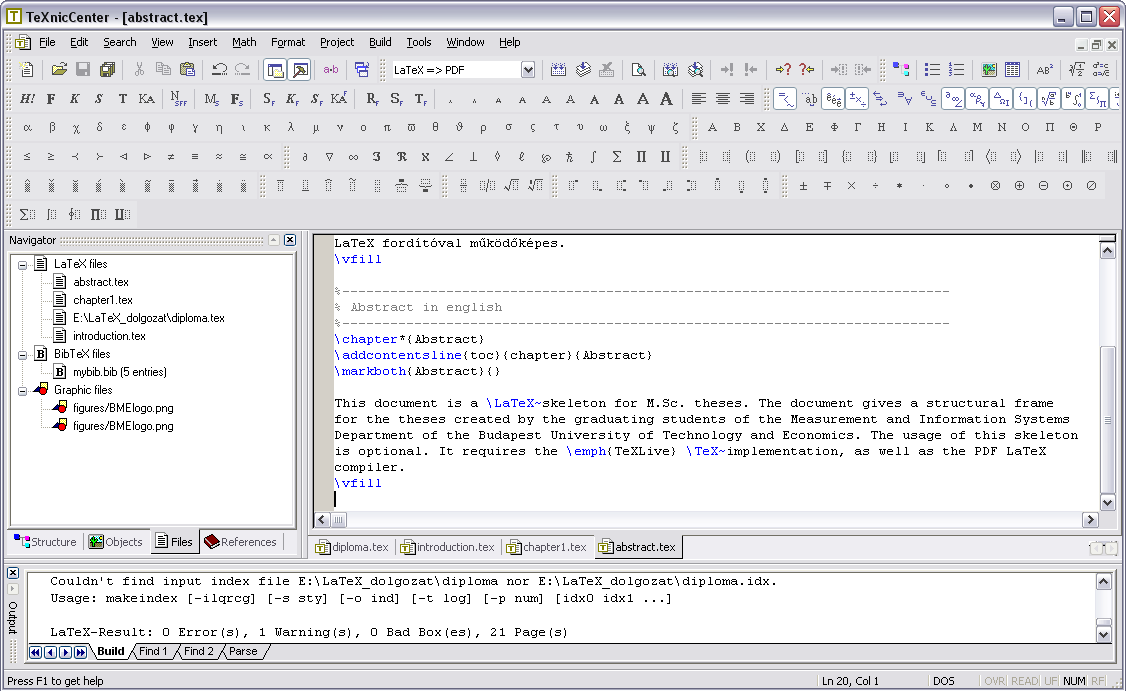
\includegraphics[width=150mm, keepaspectratio]{figures/TeXnicCenter.png}
\caption{A TeXnicCenter Windows alap� \LaTeX-szerkeszt�.} 
\label{fig:TexnicCenter}
\end{figure}
Egy m�sik haszn�lhat� Windows alap� szerkeszt�program a LEd (LaTeX Editor,\\\url{http://www.latexeditor.org/}), a TeXnicCenter azonban stabilabb, gyorsabb, �s jobban haszn�lhat�.

%----------------------------------------------------------------------------
\section{A dokumentum leford�t�sa Windows alatt}
%----------------------------------------------------------------------------
A TeXnicCenter �s a LEd kiz�r�lag szerkeszt�program (b�r az ut�bbiban DVI-n�zeget� is van), �gy a dokumentum ford�t�s�hoz sz�ks�ges eszk�z�ket nem tartalmazza. Windows alatt alapvet�en k�t lehet�s�g k�z�l �rdemes v�lasztani: MiKTeX (\url{http://miktex.org/}) �s TeXLive (\url{http://www.tug.org/texlive/}) programcsomag. Az ut�bbi m�k�dik Mac OS X, GNU/Linux alatt �s Unix-sz�rmaz�kokon is. A MiKTeX egy alapcsomag telep�t�se ut�n mindig let�lti a haszn�lt funkci�khoz sz�ks�ges, de lok�lisan hi�nyz� \TeX-csomagokat, m�g a TeXLive DVD ISO verz�ban f�rhet� hozz�. Ez a dokumentum TeXLive 2008 programcsomag seg�ts�g�vel fordult, amelynek DVD ISO verzi�ja a megadott oldalr�l let�lthet�. A sablon leford�t�s�hoz a disztrib�ci�ban szerepl� \verb+magyar.ldf+ f�jlt a \verb+http://www.math.bme.hu/latex/+ v�ltozatra kell cser�lni, vagy az ut�bbi v�ltozatot be kell m�solni a projekt-k�nyvt�rba (ahogy ezt meg is tett�k a sablonban) k�l�nben anom�li�k tapasztalhat�k a dokumentumban (pl. az �bra- �s t�bl�zat-al��r�sok form�tuma nem a be�ll�tott lesz, vagy bizonyos oldalakon megjelenik alap�telmez�sben egy fejl�c). A TeXLive 2008-at m�g nem kell k�l�n telep�teni a g�pre, elegend� DVD-r�l (vagy az ISO f�jlb�l k�zvetlen�l, pl. DaemonTools-szal) haszn�lni. 

A \TeX-eszk�z�ket tartalmaz� programcsomag bin�risainak el�r�si �tj�t minden esetben be kell �ll�tani a szerkeszt�programban, p�ld�ul TeXnicCenter eset�n legegyszer�bben a \verb+Build / Define output profiles...+ men�ponttal el�h�vott dial�gusablakban a \verb+Wizard...+ gombra kattintva tehetj�k ezt meg.

A PDF-\LaTeX~haszn�lata eset�n a gener�lt dokumentum k�zvetlen�l PDF-form�tumban �ll rendelkez�sre. Amennyiben a PDF-f�jl egy PDF-n�z�ben (pl. Adobe Acrobat Reader vagy Foxit PDF Reader) meg van nyitva, akkor a f�jlle�r�t a PDF-n�z� program tipikusan lefoglalja. Ilyen esetben a dokumentum �jraford�t�sa hiba�zenettel kil�p. Ha bez�rjuk �s �jra megnyitjuk a PDF dokumentumot, akkor pedig a PDF-n�z�k t�bbs�ge az els� oldalon nyitja meg a dokumentumot, nem a legut�bb olvasott oldalon. Ezzel szemben p�ld�ul az egyszer� �s ingyenes \textcolor{blue}{Sumatra PDF} nev� program k�pes arra, hogy a megnyitott dokumentum megv�ltoz�s�t detekt�lja, �s friss�tse a n�zetet az aktu�lis oldal megtart�s�val.

%----------------------------------------------------------------------------
\section{Eszk�z�k Linuxhoz}
%----------------------------------------------------------------------------
Linux oper�ci�s rendszer alatt is rengeteg szerkeszt�program van, pl. a KDE alap� Kile j�l haszn�lhat�. Ez ingyenesen let�lthet�, vagy �ppens�ggel az adott Linux-disztrib�ci� eleve tartalmazza, ahogyan a dokumentum ford�t�s�hoz sz�ks�ges csomagokat is. Az Ubuntu Linux disztrib�ci�k alatt p�ld�ul legt�bbsz�r a \verb+texlive-base+ csomag telep�t�s�vel haszn�lhat�k a \LaTeX-eszk�z�k.

%%----------------------------------------------------------------------------
\chapter{A dolgozat formai kivitele}
%----------------------------------------------------------------------------
Az itt tal�lhat� inform�ci�k egy r�sze a BME VIK Hallgat�i K�pviselet �ltal k�sz�tett ,,Utols� f�l�v a villanykaron'' c. munk�b�l lett kis v�ltoztat�sokkal �temelve. Az eredeti dokumentum az al�bbi linken �rhet� el: \url{http://vik-hk.bme.hu/diplomafelev-howto-2009}.

%----------------------------------------------------------------------------
\section{A dolgozat kim�rete}
%----------------------------------------------------------------------------
A minim�lis 50, az optim�lis kim�ret 60-70 oldal (f�ggel�kkel egy�tt). A b�r�l�k �s a z�r�vizsga bizotts�g sem szereti kifejezetten a t�l hossz� dolgozatokat, �gy a brutt� 90 oldalt m�r nem �rdemes t�lsz�rnyalni. Egy�bk�nt f�ggetlen�l a dolgozat kim�ret�t�l, ha a dolgozat nem �rdekfesz�t�, akkor az olvas� m�r az elej�n a v�g�t fogja v�rni. �rdemes z�rt, �nmag�ban is �rthet� m�vet alkotni.

%----------------------------------------------------------------------------
\section{A dolgozat nyelve}
%----------------------------------------------------------------------------
Mivel Magyarorsz�gon a hivatalos nyelv a magyar, ez�rt alap�rtelmez�sben magyarul kell meg�rni a dolgozatot. Aki k�lf�ldi posztgradu�lis k�pz�sben akar r�szt venni, nemzetk�zi szint� tudom�nyos kutat�st szeretne v�gezni, vagy multinacion�lis c�gn�l akar elhelyezkedni, annak c�lszer� angolul meg�rnia diplomadolgozat�t. Miel�tt a hallgat� az angol nyelv� verzi� mellett d�nt, er�sen aj�nlott m�rlegelni, hogy ez mennyi t�bbletmunk�t fog a hallgat�nak jelenteni fogalmaz�s �s nyelvhelyess�g ter�n, valamint - nem utols� sorban - hogy ez mennyi t�bbletmunk�t fog jelenteni a konzulens illetve b�r�l� sz�m�ra. Egy nehezen olvashat�, netal�n �rthetetlen sz�veg teher minden j�t�kos sz�m�ra.

%----------------------------------------------------------------------------
\section{A dokumentum nyomdatechnikai kivitele}
%----------------------------------------------------------------------------
A dolgozatot A4-es feh�r lapra nyomtatva, 2,5 centim�teres marg�val (+1~cm k�t�sbeni), 11-12 pontos bet�m�rettel, talpas bet�t�pussal �s m�sfeles sork�zzel c�lszer� elk�sz�teni.



%%----------------------------------------------------------------------------
\chapter{A \LaTeX-sablon haszn�lata}
%----------------------------------------------------------------------------
Ebben a fejezetben r�viden, implicit m�don bemutatjuk a sablon haszn�lat�nak m�dj�t, ami azt jelenti, hogy sablon haszn�lata ennek a dokumentumnak a forr�sk�dj�t tanulm�nyozva v�lik teljesen vil�goss�. Amennyiben a szoftver-keretrendszer telep�tve van, a sablon alkalmaz�sa �s a dolgozat szerkeszt�se \LaTeX-ben a sablon seg�ts�g�vel tapasztalataink szerint j�val hat�konyabb, mint egy WYSWYG (\emph{What You See is What You Get}) t�pus� sz�vegszerkeszt� eset�n (pl. Microsoft Word, OpenOffice).

%----------------------------------------------------------------------------
\section{C�mk�k �s hivatkoz�sok}
%----------------------------------------------------------------------------
A \LaTeX~dokumentumban c�mk�ket (\verb+\label+) rendelhet�nk �br�khoz, t�bl�zatokhoz, fejezetekhez, list�khoz, k�pletekhez stb. Ezekre a dokumentum b�rmely r�sz�ben hivatkozhatunk, a hivatkoz�sok automatikusan felold�sra ker�lnek.

A sablonban makr�kat defini�ltunk a hivatkoz�sok megk�nny�t�s�hez. Ennek megfelel�en minden �bra (\emph{figure}) c�mk�je \verb+fig:+ kulcssz�val kezd�dik, m�g minden t�bl�zat (\emph{table}), k�plet (\emph{equation}), fejezet (\emph{section}) �s lista (\emph{listing}) rendre a \verb+tab:+, \verb+eq:+, \verb+sect:+ �s \verb+listing:+ kulcssz�val kezd�dik, �s a kulcsszavak ut�n tetsz�legesen v�lasztott c�mke haszn�lhat�. Ha ezt a konvenci�t betartjuk, akkor az el�bbi objektumok sz�m�ra rendre a \verb+\figref+, \verb+\tabref+, \verb+\eqref+, \verb+\sectref+ �s \verb+\listref+ makr�kkal hivatkozhatunk. A makr�k param�tere a c�mke, amelyre hivatkozunk (a kulcssz� n�lk�l). Az �sszes eml�tett hivatkoz�st�pus, bele�rtve az \verb+\url+ kulcssz�val bevezetett web-hivatkoz�sokat is a  \verb+hyperref+\footnote{Seg�ts�g�vel a dokumentumban megjelen� hivatkoz�sok nem csak dinamikuss� v�lnak, de sz�nezhet�k is, b�vebbet err�l a csomag dokument�ci�j�ban tal�lunk. Ez egy�ttal egy p�lda l�bjegyzet �r�s�ra.} csomagnak k�sz�nhet�en akt�vak a legt�bb PDF-n�zeget�ben, r�juk kattintva a dokumentum megfelel� oldal�ra ugrik a PDF-n�z� vagy a megfelel� linket megnyitja az alap�rtelmezett b�ng�sz�vel. A \verb+hyperref+ csomag a kimeneti PDF-dokumentumba k�nyvjelz�ket is k�sz�t a tartalomjegyz�kb�l. Ez egy szint�n akt�v tartalomjegyz�k, amelynek elemeire kattintva a n�zeget� behozza a kiv�lasztott fejezetet.

%----------------------------------------------------------------------------
\section{�br�k �s t�bl�zatok}
%----------------------------------------------------------------------------
A k�peket PDFLaTeX eset�n a vesztes�gmentes PNG, valamint a vesztes�ges JPEG form�tumban �rdemes elmenteni. Az EPS (PostScript) vektorgrafikus k�pform�tum beilleszt�s�t a PDFLatex k�zvetlen�l nem t�mogatja. Ehelyett egy lehet�s�g 200 dpi, vagy ann�l nagyobb felbont�sban raszteriz�lni a k�pet, �s PNG form�tumban elmenteni. Az egyes k�pek m�rete �ltal�ban nem, de sok k�p eset�n a dokumentum �sszm�rete �gy m�r szignifik�ns is lehet. A dokumentumban felhaszn�lt k�pf�jlokat a dokumentum forr�sa mellett �rdemes tartani, archiv�lni, mivel ezek hi�ny�ban a dokumentum nem fordul �jra. Ha lehet, a vektorgrafikus k�peket vektorgrafikus form�tumban is �rdemes elmenteni az �jrafelhaszn�lhat�s�g (az �tszerkeszthet�s�g) �rdek�ben.

Kapcsol�si rajzok legt�bbsz�r kim�solhat�k egy vektorgrafikus programba (pl. CorelDraw) �s onnan nagyobb felbont�ssal raszteriz�lva kimenthat�k PNG form�tumban. Ugyanakkor kiv�l� �br�k k�sz�thet�k Microsoft Visio vagy hasonl� program haszn�lat�val is: Visio-b�l az �br�k k�zvetlen�l PNG-be is menthet�k.

Lehet�s�geink Matlab �br�k eset�n:
\begin{itemize}
	\item K�perny�lop�s (\emph{screenshot}) is elfogadhat� min�s�g� lehet a dokumentumban, de �ltal�ban jobb felbont�st is el lehet �rni m�s m�dszerrel.
	\item A Matlab �br�t a \verb+File/Save As+ opci�val lementhetj�k PNG form�tumban (ugyanaz itt is �rv�nyes, mint kor�bban, ez�rt nem javasoljuk).
	\item A Matlab �br�t az \verb+Edit/Copy figure+ opci�val kim�solhatjuk egy vektorgrafikus programba is �s onnan nagyobb felbont�ssal raszteriz�lva kimenthatj�k PNG form�tumban (nem javasolt).
	\item Javasolt megold�s: az �br�t a \verb+File/Save As+ opci�val EPS \emph{vektorgrafikus} form�tumban elmentj�k, PDF-be konvert�lva beillesztj�k a dolgozatba.
\end{itemize}
Az EPS k�p az \verb+epstopdf+ programmal\footnote{a kor�bban eml�tett \LaTeX-disztrib�ci�kban megtal�lhat�} konvert�lhat� PDF form�tumba. C�lszer� egy batch-f�jlt k�sz�teni az �sszes EPS �bra leford�t�s�ra az al�bbi m�don (ez Windows alatt m�k�dik).
\begin{lstlisting}[frame=single,float=!ht]
@echo off
for %%j in (*.eps) do (
echo converting file "%%j"
epstopdf "%%j"
)
echo done .
\end{lstlisting}

Egy ilyen parancsf�jlt (\verb+convert.cmd+) elhelyezt�k a sablon \verb+figures\eps+ k�nyvt�r�ba, �gy a felhaszn�l�nak csak annyi a dolga, hogy a \verb+figures\eps+ k�nyvt�rba kimenti az EPS form�tum� vektorgrafikus k�pet, majd lefuttatja a \verb+convert.cmd+ parancsf�jlt, ami PDF-be konvert�lja az EPS f�jlt.

Ezek ut�n a PDF-�br�t ugyan�gy lehet a dokumentumba beilleszteni, mint a PNG-t vagy a JPEG-et. A megold�s el�nye, hogy a leford�tott dokumentumban is vektorgrafikusan t�rol�dik az �bra, �gy a m�rete j�val kisebb, mintha raszteriz�ltuk volna beilleszt�s el�tt. Ez a m�dszer minden -- az EPS form�tumot ismer� -- vektorgrafikus program (pl. CorelDraw) eset�n is haszn�lhat�.

A k�pek beilleszt�s�re az \sectref{LatexTools}. fejezetben mutattunk be p�ld�t (\figref{TexnicCenter}~�bra). Az el�z� mondatban egy�ttal az automatikusan felold�d� �brahivatkoz�sra is l�thatunk p�ld�t. T�bb k�pf�jlt is beilleszthet�nk egyetlen �br�ba. Az egyes k�pek k�z�tti horizont�lis �s vertik�lis marg�t metrikusan szab�lyozhatjuk (\figref{HVSpaces}~�bra). Az �br�k elhelyez�s�t sz�mtalan tipogr�fiai szab�ly egyidej� teljes�t�s�vel a ford�t� maga v�gzi, a dokumentum �r�ja csak preferenci�it jelezheti a ford�t� fel� (olykor ez bossz�s�got is okozhat, ilyenkor pl. a k�p m�ret�vel lehet j�tszani).

\begin{figure}[!ht]
\centering
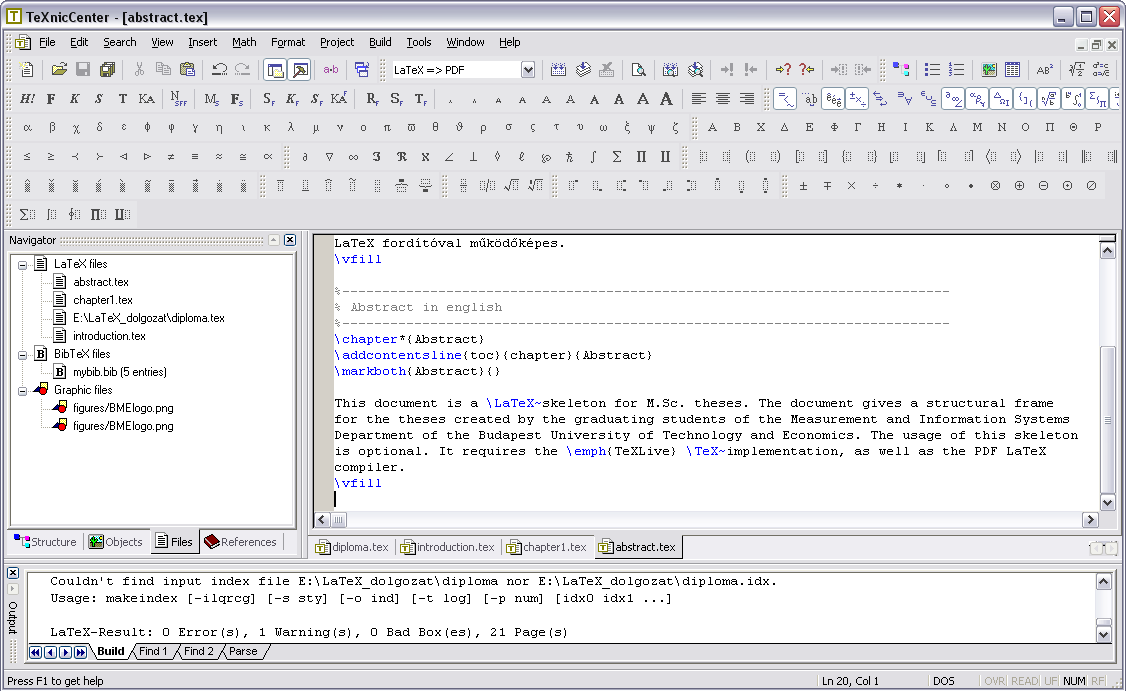
\includegraphics[width=67mm, keepaspectratio]{figures/TeXnicCenter.png}\hspace{1cm}
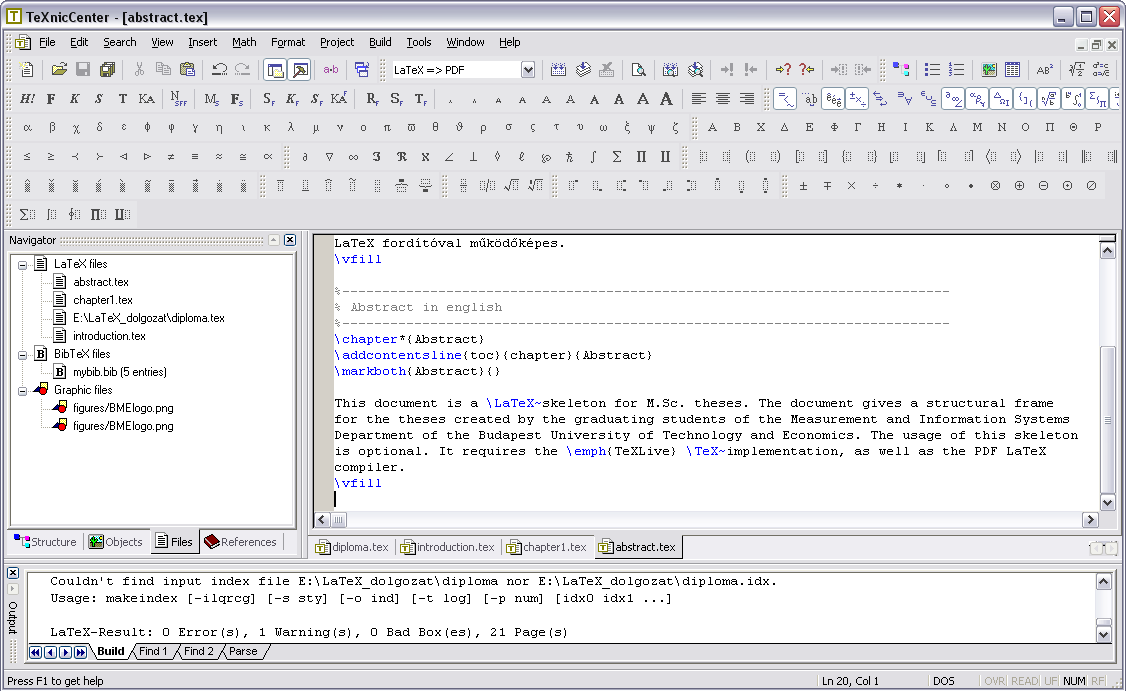
\includegraphics[width=67mm, keepaspectratio]{figures/TeXnicCenter.png}\\\vspace{5mm}
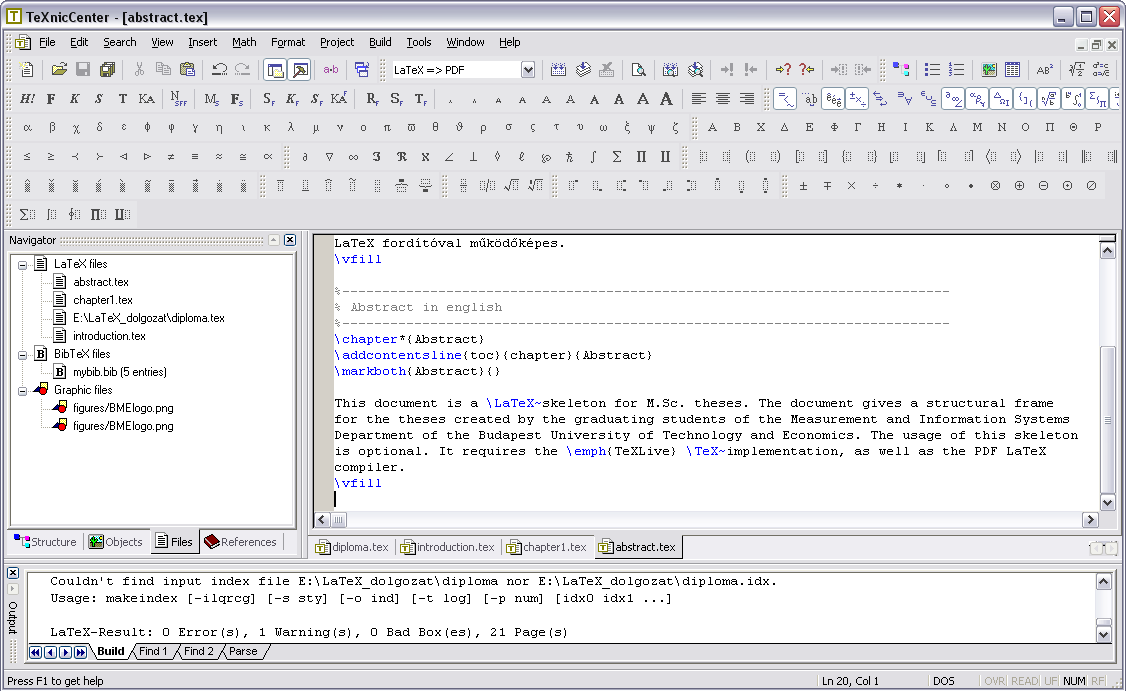
\includegraphics[width=67mm, keepaspectratio]{figures/TeXnicCenter.png}\hspace{1cm}
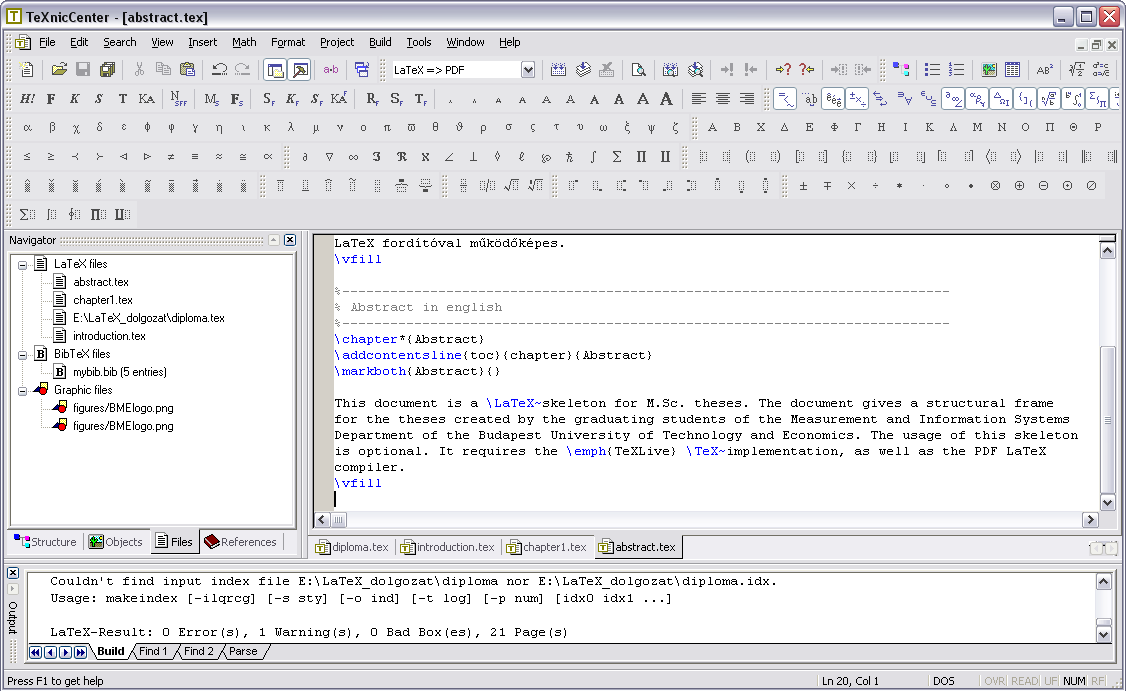
\includegraphics[width=67mm, keepaspectratio]{figures/TeXnicCenter.png}
\caption{T�bb k�pf�jl beilleszt�se eset�n t�rk�z�ket is �rdemes haszn�lni.} 
\label{fig:HVSpaces}
\end{figure}

A t�bl�zatok haszn�lat�ra a \tabref{TabularExample}~t�bl�zat mutat p�ld�t.
A t�bl�zat c�mk�je nem v�letlen�l ker�lt a t�bl�zat f�l�, ez a szokv�nyos.
\begin{table}[ht]
	\footnotesize
	\centering
	\caption{Az �rajel-gener�tor chip �rajel-kimenetei.} \label{tab:SysClocks}
	\begin{tabular}{ | l | c | c |}
	\hline
	�rajel & Frekvencia & C�l pin \\ \hline
	CLKA & 100 MHz & FPGA CLK0\\
	CLKB & 48 MHz  & FPGA CLK1\\
	CLKC & 20 MHz  & Processzor\\
	CLKD & 25 MHz  & Ethernet chip \\
	CLKE & 72 MHz  & FPGA CLK2\\
	XBUF & 20 MHz  & FPGA CLK3\\
	\hline
	\end{tabular}
	\label{tab:TabularExample}
\end{table}


%----------------------------------------------------------------------------
\section{Felsorol�sok �s list�k}
%----------------------------------------------------------------------------
Sz�mozatlan felsorol�sra mutat p�ld�t a jelenlegi bekezd�s:
\begin{itemize}
	\item \emph{els� bajusz:} ide lehetne �rni az els� elem kifej�s�t,
	\item \emph{m�sodik bajusz:} ide lehetne �rni a m�sodik elem kifej�s�t,
	\item \emph{ez meg egy szak�ll:} ide lehetne �rni a harmadik elem kifej�s�t.
\end{itemize}

Sz�mozott felsorol�st is k�sz�thet�nk az al�bbi m�don:
\begin{enumerate}
	\item \emph{els� bajusz:} ide lehetne �rni az els� elem kifej�s�t, �s ez a kifejt�s �gy n�z ki, ha t�bb sorosra sikeredik,
	\item \emph{m�sodik bajusz:} ide lehetne �rni a m�sodik elem kifej�s�t,
	\item \emph{ez meg egy szak�ll:} ide lehetne �rni a harmadik elem kifej�s�t.
\end{enumerate}
A felsorol�sokban sorok v�g�n vessz�, az utols� sor v�g�n pedig pont a szok�sos �r�sjel. Ez al�l kiv�telt k�pezhet, ha az egyes elemek t�bb teljes mondatot tartalmaznak.

List�kban a dolgozat sz�veg�t�l elk�l�n�tend� k�dr�szleteket, programsorokat, pszeudo-k�dokat jelen�thet�nk meg (\listref{Example}~lista). 
\begin{lstlisting}[frame=single,float=!ht,caption=A fenti sz�mozott felsorol�s \LaTeX- forr�sk�dja, label=listing:Example]
\begin{enumerate}
	\item \emph{els� bajusz:} ide lehetne �rni az els� elem kifej�s�t, 
	�s ez a kifejt�s �gy n�z ki, ha t�bb sorosra sikeredik,
	\item \emph{m�sodik bajusz:} ide lehetne �rni a m�sodik elem kifej�s�t,
	\item \emph{ez meg egy szak�ll:} ide lehetne �rni a harmadik elem kifej�s�t.
\end{enumerate}
\end{lstlisting}
A lista keret�t, h�tt�rsz�n�t, eg�sz st�lus�t megv�laszthatjuk. R�ad�sul k�l�nf�le programnyelveket �s a nyelveken bel�l kulcsszavakat is defini�lhatunk, ha sz�ks�ges. Err�l b�vebbet a \verb+listings+ csomag hivatalos le�r�s�ban tal�lhatunk.

%----------------------------------------------------------------------------
\section{K�pletek}
%----------------------------------------------------------------------------
Ha egy formula nem t�ls�gosan hossz�, �s nem akarjuk hivatkozni a sz�vegb�l, mint p�ld�ul a $e^{i\pi}+1=0$ k�plet, \emph{sz�vegk�zi k�pletk�nt} szok�s le�rni. Csak, hogy m�sik p�ld�t is l�ssunk, az $U_i=-d\Phi/dt$ Faraday-t�rv�ny a $\rot E=-\frac{dB}{dt}$ differenci�lis alakban adott Maxwell-egyenlet fel�letre vett integr�lj�b�l vezethet� le. L�that�, hogy a \LaTeX-ford�t� a sork�z�ket betartja, �gy a sz�veg szed�se eszt�tikus marad sz�vegk�zi k�pletek haszn�lata eset�n is.

K�pletek eset�n az �ltal�nos konvenci�, hogy a kisbet�k skal�rt, a kis f�lk�v�r bet�k ($\mathbf{v}$) oszlopvektort -- �s ennek megfelel�en $\mathbf{v}^T$ sorvektort -- a kapit�lis f�lk�v�r bet�k ($\mathbf{V}$) m�trixot jel�lnek. Ha ett�l el szeretn�nk t�rni, akkor az alkalmazni k�v�nt jel�l�sm�dot c�lszer� k�l�n alfejezetben defini�lni. Ennek megfelel�en, amennyiben $\mathbf{y}$ jel�li a m�r�sek vektor�t, $\mathbf{\vartheta}$ a param�terek vektor�t �s $\hat{\mathbf{y}}=\mathbf{X}\vartheta$ a param�terekben line�ris modellt, akkor a \emph{Least-Squares} �rtelemben optim�lis param�terbecsl� $\hat{\mathbf{\vartheta}}_{LS}=(\mathbf{X}^T\mathbf{X})^{-1}\mathbf{X}^T\mathbf{y}$ lesz.

Emellett kiemelt, sorsz�mozott k�pleteket is megadhatunk, enn�l az \verb+equation+ �s a \verb+eqnarray+ k�rnyezetek helyett a korszer�bb \verb+align+ k�rnyezet alkalmaz�s�t javasoljuk (t�bb okb�l, k�l�nf�le probl�m�k elker�l�se v�gett, amelyekre most nem t�r�nk ki). Teh�t
\begin{align}
\dot{\mathbf{x}}&=\mathbf{A}\mathbf{x}+\mathbf{B}\mathbf{u},\\
\mathbf{y}&=\mathbf{C}\mathbf{x},
\end{align}
ahol $\mathbf{x}$ az �llapotvektor, $\mathbf{y}$ a m�r�sek vektora �s $\mathbf{A}$, $\mathbf{B}$ �s $\mathbf{C}$ a rendszert le�r� param�term�trixok. Figyelj�k meg, hogy a k�t egyenletben az egyenl�s�gjelek egym�shoz igaz�tva jelennek meg, mivel a mindkett�t az \& karakter el�zi meg a k�dban. Lehet�s�g van sz�mozatlan kiemelt k�plet haszn�lat�ra is, p�ld�ul
\begin{align}
\dot{\mathbf{x}}&=\mathbf{A}\mathbf{x}+\mathbf{B}\mathbf{u},\nonumber\\
\mathbf{y}&=\mathbf{C}\mathbf{x}\nonumber.
\end{align}
M�trixok fel�r�s�ra az $\mathbf{A}\mathbf{x}=\mathbf{b}$ inhomog�n line�ris egyenlet r�szletes kifejt�s�vel mutatunk p�ld�t:
\begin{align}
\begin{bmatrix}
a_{11} & a_{12} & \dots & a_{1n}\\
a_{21} & a_{22} & \dots & a_{2n}\\
\vdots & \vdots & \ddots & \vdots\\
a_{m1} & a_{m2} & \dots & a_{mn}
\end{bmatrix}
\begin{pmatrix}x_1\\x_2\\\vdots\\x_n\end{pmatrix}=
\begin{pmatrix}b_1\\b_2\\\vdots\\b_m\end{pmatrix}.
\end{align}
A \verb+\frac+ utas�t�s hat�konys�g�t egy �ltal�nos m�sodfok� tag �tviteli f�ggv�ny�n kereszt�l mutatjuk be, azaz
\begin{align}
W(s)=\frac{A}{1+2T\xi s+s^2T^2}.
\end{align}
A matematikai m�d minden szimb�lum�nak �s k�pess�g�nek a bemutat�s�ra term�szetesen itt nincs lehet�s�g, de gyors referenciak�nt hat�konyan haszn�lhat�k a k�vetkez� linkek:\\
\indent\url{http://www.artofproblemsolving.com/LaTeX/AoPS_L_GuideSym.php},\\
\indent\url{http://www.ctan.org/tex-archive/info/symbols/comprehensive/symbols-a4.pdf},\\
\indent\url{ftp://ftp.ams.org/pub/tex/doc/amsmath/short-math-guide.pdf}.\\
Ez pedig itt egy magyar�zat, hogy mi�rt �rdemes \verb+align+ k�rnyezetet haszn�lni:\\
\indent\url{http://texblog.net/latex-archive/maths/eqnarray-align-environment/}.

%----------------------------------------------------------------------------
\section{Irodalmi hivatkoz�sok}\label{sect:HowtoReference}
%----------------------------------------------------------------------------
Egy \LaTeX dokumentumban az irodalmi hivatkoz�sok defin�ci�j�nak k�t m�dja van. Az egyik a \verb+\thebibliograhy+ k�rnyezet haszn�lata a dokumentum v�g�n, az \verb+\end{document}+ lez�r�s el�tt.
\begin{lstlisting}[frame=single,float=!ht]
\begin{thebibliography}{9}

\bibitem{Lamport94} Leslie Lamport, \emph{\LaTeX: A Document Preparation System}. 
Addison Wesley, Massachusetts, 2nd Edition, 1994.

\end{thebibliography}
\end{lstlisting}

Ezek ut�n a dokumentumban a \verb+\cite{Lamport94}+ utas�t�ssal hivatkozhatunk a forr�sra. A fenti megad�s viszonylag k�tetlen, a szerz� maga form�zza az irodalomjegyz�ket. 

Egy sokkal professzion�lisabb m�dszer a BiB\TeX~haszn�lata, ez�rt ez a sablon is ezt t�mogatja. Ebben az esetben egy k�l�n sz�veges adatb�zisban defini�ljuk a forr�smunk�kat, �s egy k�l�n st�lusf�jl hat�rozza meg az irodalomjegyz�k kin�zet�t. Ez, �sszhangban azzal, hogy k�l�n form�tumkonvenci� hat�rozza meg a foly�irat-, a k�nyv-, a konferenciacikk- stb. hivatkoz�sok kin�zet�t az irodalomjegyz�kben (a sablon haszn�lata eset�n ezzel nem is kell foglalkoznia a hallgat�nak, de az eredm�nyt c�lszer� ellen�rizni). A felhaszn�lt hivatkoz�sok adatb�zisa egy \verb+.bib+ kiterjeszt�s� sz�veges f�jl, amelynek szerkezet�t a \listref{Bibtex} k�dr�szlet demonstr�lja. A forr�smunk�k bevitelekor a sor v�gi vessz�k k�l�n figyelmet ig�nyelnek, mert hi�nyuk a BiB\TeX-ford�t� hiba�zenet�t eredm�nyezi. A forr�smunk�kat t�pus szerinti kulcssz� vezeti be (\verb+@book+ k�nyv, \verb+@inproceedings+ konferenciakiadv�nyban megjelent cikk, \verb+@article+ foly�iratban megjelent cikk, \verb+@techreport+ valamelyik egyetem gondoz�s�ban megjelent m�szaki tanulm�ny, \verb+@manual+ m�szaki dokument�ci� eset�n stb.). Nemcsak a megjelen�s st�lusa, de a k�telez�en megadand� mez�k is t�pusr�l-t�pusra v�ltoznak. Egy j�l haszn�lhat� referencia a \url{http://en.wikipedia.org/wiki/BibTeX} oldalon tal�lhat�.
\begin{lstlisting}[frame=single,float=!ht,caption=P�lda sz�veges irodalomjegyz�k-adatb�zisra BiBTeX haszn�lata eset�n., label=listing:Bibtex]
@BOOK{Wettl04,
  author="Ferenc Wettl and Gyula Mayer and P�ter Szab�",
  title="\LaTeX~k�zik�nyv",
  publisher="Panem K�nyvkiad�",
  year=2004
}
@ARTICLE{Candy86,
  author ="James C. Candy",
  title  ="Decimation for Sigma Delta Modulation",
  journal="{IEEE} Trans.\ on Communications",
  volume =34,
  number =1,
  pages  ="72--76",
  month  =jan,
  year   =1986,
}
@INPROCEEDINGS{Lee87,
  author =       "Wai L. Lee and Charles G. Sodini",
  title =        "A Topology for Higher Order Interpolative Coders",
  booktitle =    "Proc.\ of the IEEE International Symposium on 
  Circuits and Systems",
  year =         1987,
  vol =          2,
  month =        may # "~4--7",
  address =      "Philadelphia, PA, USA",
  pages =        "459--462"
}
@PHDTHESIS{KissPhD,
  author =   "Peter Kiss",
  title =    "Adaptive Digital Compensation of Analog Circuit Imperfections 
  for Cascaded Delta-Sigma Analog-to-Digital Converters",
  school =   "Technical University of Timi\c{s}oara, Romania",
  month =    apr,
  year =     2000
}
@MANUAL{Schreier00,
  author = "Richard Schreier",
  title  = "The Delta-Sigma Toolbox v5.2",
  organization = "Oregon State University",
  year   = 2000,
  month  = jan,
  note   ="\newline URL: http://www.mathworks.com/matlabcentral/fileexchange/"
}
@MISC{DipPortal,
	author="Budapesti {M}�szaki �s {G}azdas�gtudom�nyi {E}gyetem 
	{V}illamosm�rn�ki �s {I}nformatikai {K}ar",
  title="{D}iplomaterv port�l (2011 febru�r 26.)",
  howpublished="\url{http://diplomaterv.vik.bme.hu/}",
}}
\end{lstlisting}

A st�lusf�jl egy \verb+.sty+ kiterjeszt�s� f�jl, de ezzel l�nyeg�ben nem kell foglalkozni, mert vannak be�p�tett st�lusok, amelyek j�l haszn�lhat�k. Ez a sablon a BiB\TeX-et haszn�lja, a hozz� tartoz� adatb�zisf�jl a \verb+mybib.bib+ f�jl. Megfigyelhet�, hogy az irodalomjegyz�ket a dokumentum v�g�re (a \verb+\end{document}+ utas�t�s el�) beillesztett \verb+\bibliography{mybib}+ utas�t�ssal hozhatjuk l�tre, a st�lus�t pedig ugyanitt a  \verb+\bibliographystyle{plain}+ utas�t�ssal adhatjuk meg. Ebben az esetben a \verb+plain+ el�re defini�lt st�lust haszn�ljuk (a sablonban is ezt �ll�tottuk be). A \verb+plain+ st�luson k�v�l term�szetesen sz�mtalan m�s el�re defini�lt st�lus is l�tezik. Mivel a \verb+.bib+ adatb�zisban ezeket megadtuk, a BiB\TeX-ford�t� is meg tudja k�l�nb�ztetni a szerz�t a c�mt�l �s a kiad�t�l, �s ez alapj�n automatikusan gener�l�dik az irodalomjegyz�k a st�lusf�jl �ltal meghat�rozott st�lusban.

Az egyes forr�smunk�kra a sz�vegb�l tov�bbra is a \verb+\cite+ paranccsal tudunk hivatkozni, �gy a \listref{Bibtex} k�dr�szlet eset�n a hivatkoz�sok rendre \verb+\cite{Wettl04}+, \verb+\cite{Candy86}+, \verb+\cite{Lee87}+, \verb+\cite{KissPhD}+, \verb+\cite{Schreirer00}+ �s \verb+\cite{DipPortal}+. Az irodalomjegyz�kben alap�rtelmez�sben csak azok a forr�smunk�k jelennek meg, amelyekre tal�lhat� hivatkoz�s a sz�vegben, �s ez �gy alapvet�en helyes is, hiszen olyan forr�smunk�kat nem illik az irodalomjegyz�kbe �rni, amelyekre nincs hivatkoz�s.

Mivel a ford�t�si folyamat sor�n t�bb l�p�sben old�dnak fel a szimb�lumok, ez�rt gyakran t�bbsz�r (TeXLive �s TeXnicCenter eset�n 2-3-szor) is le kell ford�tani a dokumentumot. Ilyenkor ez els� 1-2 ford�t�s esetleg szimb�lum-felold�sra vonatkoz� figyelmeztet� �zenettel z�rul. Ha hiba�zenettel z�rul b�rmelyik ford�t�s, akkor nincs �rtelme megism�telni, hanem a hib�t kell megkeresni. A \verb+.bib+ f�jl megv�ltoztat�skor sokszor nincs hat�sa a v�ltoztat�snak azonnal, mivel nem mindig fut �jra a BibTeX ford�t�. Ez�rt c�lszer� a v�ltoztat�s ut�n azt manu�lisan is lefuttatni (TeXnicCenter eset�n \verb+Build/BibTeX+).

Hogy a sz�vegbe �gyazott hivatkoz�sok kin�zet�t demonstr�ljuk, itt most sorban meghivatkozzuk a \cite{Wettl04}, \cite{Candy86}, \cite{Lee87}, \cite{KissPhD} �s az \cite{Schreier00} forr�smunk�t, valamint az \cite{DipPortal} weboldalt.

Megjegyzend�, hogy az �kezetes magyar bet�ket is tartalmaz� \verb+.bib+ f�jl az \verb+inputenc+ csomaggal bet�lt�tt \verb+latin2+ bet�k�szlet miatt ford�that�. Ugyanez a \verb+.bib+ f�jl hiba�zenettel fordul egy olyan dokumentumban, ami nem tartalmazza a \verb+\usepackage[latin2]{inputenc}+ sort. Speci�lis ig�ny eset�n az irodalmi adatb�zis �ltal�nosabb �rv�ny�v� tehet�, ha az �kezetes bet�ket speci�lis latex karakterekkel helyettes�tj�k a \verb+.bib+ f�jlban, pl. � helyett \verb+\'{a}+-t vagy � helyett \verb+\H{o}+-t �runk. 

Oldalt�r�s k�vetkezik (ld. forr�s).
\newpage

%----------------------------------------------------------------------------
\section{A dolgozat szerkezete �s a forr�sf�jlok}
%----------------------------------------------------------------------------
A diplomatervsablon (a kari ir�nyelvek szerint) az al�bbi f� fejezetekb�l �ll:
\begin{enumerate}
	\item 1 oldalas \emph{t�j�koztat�} a szakdolgozat/diplomaterv szerkezet�r�l (\verb+guideline.tex+), ami a v�gs� dolgozatb�l t�rlend�,
	\item \emph{feladatki�r�s} (\verb+project.tex+), a dolgozat nyomtatott verz�j�ban ennek a hely�re ker�l a tansz�k �ltal kiadott, a tansz�kvezet� �ltal al��rt feladatki�r�s, a dolgozat elektronikus verzi�j�ba pedig a feladatki�r�s egy�ltal�n ne ker�lj�n bele, azt k�l�n t�lti fel a tansz�k a diplomaterv-honlapra,
	\item \emph{c�moldal} (\verb+titlepage.tex+),
	\item \emph{tartalomjegyz�k} (\verb+diploma.tex+),
	\item a diplomatervez� \emph{nyilatkozat}a az �n�ll� munk�r�l (\verb+declaration.tex+),
	\item 1-2 oldalas tartalmi \emph{�sszefoglal�} magyarul �s angolul, illetve elk�sz�thet� m�g tov�bbi nyelveken is (\verb+abstract.tex+),
	\item \emph{bevezet�s}: a feladat �rtelmez�se, a tervez�s c�lja, a feladat indokolts�ga, a diplomaterv fel�p�t�s�nek r�vid �sszefoglal�sa (\verb+introduction.tex+),
	\item sorsz�mmal ell�tott \emph{fejezetek}: a feladatki�r�s pontos�t�sa �s r�szletes elemz�se, el�zm�nyek (irodalomkutat�s, hasonl� alkot�sok), az ezekb�l levonhat� k�vetkeztet�sek, a tervez�s r�szletes le�r�sa, a d�nt�si lehet�s�gek �rt�kel�se �s a v�lasztott megold�sok indokl�sa, a megtervezett m�szaki alkot�s �rt�kel�se, kritikai elemz�se, tov�bbfejleszt�si lehet�s�gek (\verb+chapter{1,2..n}.tex+),
	\item esetleges \emph{k�sz�netnyilv�n�t�s}ok (\verb+acknowledgement.tex+),
	\item r�szletes �s pontos \emph{irodalomjegyz�k} (ez a sablon eset�ben automatikusan gener�l�dik a \verb+diploma.tex+ f�jlban elhelyezett \verb+\bibliography+ utas�t�s hat�s�ra, a \sectref{HowtoReference}. fejezetben le�rtak szerint),
	\item \emph{f�ggel�kek} (\verb+appendices.tex+).
\end{enumerate}

A sablonban a fejezetek a \verb+diploma.tex+ f�jlba vannak beillesztve \verb+\include+ utas�t�sok seg�ts�g�vel. Lehet�s�g van arra, hogy csak az �ppen szerkeszt�s alatt �ll� \verb+.tex+ f�jlt ford�tsuk le, ezzel ler�vid�tve a ford�t�si folyamatot. Ezt a lehet�s�get az al�bbi k�dr�szlet biztos�tja a \verb+diploma.tex+ f�jlban.
\begin{lstlisting}[frame=single,float=!ht]
\includeonly{
	guideline,%
	project,%
	titlepage,%
	declaration,%
	abstract,%
	introduction,%
	chapter1,%
	chapter2,%
	chapter3,%
	acknowledgement,%
	appendices,%
}
\end{lstlisting}

Ha az al�bbi k�dr�szletben az egyes sorokat a \verb+%+ szimb�lummal kikommentezz�k, akkor a megfelel� \verb+.tex+ f�jl nem fordul le. Az oldalsz�mok �s a tartalomjegy�k term�szetesen csak akkor billennek helyre, ha a teljes dokumentumot leford�tjuk.

%----------------------------------------------------------------------------
\newpage
\section{Alapadatok megad�sa}
%----------------------------------------------------------------------------
A diplomaterv alapadatait (c�m, szerz�, konzulens, konzulens titulusa) a \verb+diploma.tex+ f�jlban lehet megadni az al�bbi k�dr�szlet m�dos�t�s�val.
\begin{lstlisting}[frame=single,float=!ht]
\newcommand{\vikszerzo}{B�dis-Szomor� Andr�s}
\newcommand{\vikkonzulens}{dr.~Konzulens Elem�r}
\newcommand{\vikcim}{Elektronikus terel�k}
\newcommand{\viktanszek}{M�r�stechnika �s Inform�ci�s Rendszerek Tansz�k}
\newcommand{\vikdoktipus}{Diplomaterv}
\newcommand{\vikdepartmentr}{B�dis-Szomor� Andr�s}
\end{lstlisting}

%----------------------------------------------------------------------------
\section{�j fejezet �r�sa}
%----------------------------------------------------------------------------
A f�fejezetek k�l�n \verb+chapter{1..n}.tex+ f�jlban foglalnak helyet. A sablonhoz 3 fejezet k�sz�lt. Tov�bbi f�fejezeteket �gy hozhatunk l�tre, ha �j \verb+chapter{i}.tex+ f�jlt k�sz�t�nk a fejezet sz�m�ra, �s a \verb+diploma.tex+ f�jlban, a \verb+\include+ �s \verb+\includeonly+ utas�t�sok argumentum�ba felvessz�k az �j \verb+.tex+ f�jl nev�t.






%%----------------------------------------------------------------------------
\chapter*{K�sz�netnyilv�n�t�s}\addcontentsline{toc}{chapter}{K�sz�netnyilv�n�t�s}
%----------------------------------------------------------------------------

Ez nem k�telez�, ak�r t�r�lhet� is. Ha a szerz� sz�ks�g�t �rzi, itt lehet k�sz�netet nyilv�n�tani azoknak, akik hozz�j�rultak munk�jukkal ahhoz, hogy a hallgat� a szakdolgozatban vagy diplomamunk�ban le�rt feladatokat sikeresen elv�gezze. A konzulensnek val� k�sz�netnyilv�n�t�s sem k�telez�, a konzulensnek hivatalosan is dolga, hogy a hallgat�t konzult�lja.
%\clearpage
\begin{center}
\large
\textbf{Szakmai gyakorlat beszámoló}\\
Solymos Balázs - O60Z1K
\end{center}

\section*{Bevezető}

A szakmai gyakorlatot(Bsc villamosmérnök) idén nyáron végeztem a Qrypt Solutions kft. -nél. A szakmai konzulensem/mentorom Bacsárdi László volt, a gyakorlatom 2017 május végétől 6 hétig, 2017 július elejéig tartott. Azért választottam ezt a helyet a szakmai gyakorlatom elvégzésére, mert itt lehetőségem volt a szűkebb személyes érdeklődési körömbe is eső témával foglalkozni. Ez a téma a kvantumkommunikáció, melynek egyéb ágazataival valamelyest megismerkedtem korábban már az egyetemen az önálló laborom keretében,többek közt az ottani konzulensem ajánlotta ezt a lehetőséget, amivel később örömmel éltem. 

\section*{A gyakorlat}

A gyakorlat első hetében a szükséges adminisztráció elvégzése után, megkaptam az első elvégzendő feladatom, amivel az utána lévő hetekben foglalkoztam, valamint a hét végére egy belépő kártyát is a laborba, ahol a továbbiakban gyakorlatom végeztem, valamint kaptam egy asztalt erre a célra. Mivel lehetőségem volt a saját laptopom használatára a munka során ezért az asztalhoz biztosított eszközök közül csak egy plusz monitort használtam. Az itt töltött hat hetem feladatok szempontjából(később részletezve) két főbb részre osztható. Az első 3 hétben a kvantumkommunikáció helyzetét vizsgáltam Európában, különös figyelmet fordítva a kutatási támogatási rendszernek és végül a szerzett információkból készítettem egy rövidebb magyar nyelvű összefoglalót. A gyakorlat fennmaradó részében pedig kvantumkommunikáció fejlődését, helyzetét valamint a hozzá kapcsolódó fontosabb jelenségek bemutatását segítő anyagokat készítettem, melyek segítségével elkészült egy teljes plakátterv is. A feladatok egyéni feladatjaim voltak, ebből következik, hogy a gyakorlat alatt kizárólag önállóan dolgoztam, időnkénti konzultációval, valamint külső véleményezéssel megszakítva. Ezen tények miatt(saját laptop, önálló főleg irodalomkutatásból álló feladat) lehetőségem volt a laboron kívüli aktív munkavégzésre is, amit segített a flexibilisebb időbeosztás is, de hamar úgy találtam, hogy a labor által nyújtott környezet a legalkalmasabb számomra, különösen mikor a feladatokhoz szükséges információgyűjtéssel már végeztem.

\section*{Feladatok}

\subsection *{Quantum Manifesto}

A gyakorlat első felében feladatnak kaptam a közelmúltban közéttet Quantum Manifesto dokumentum, valamint az ehhez kapcsolódó Európai Uniós kutatási támogatási tervek, célkitűzések ismertetését, továbbá a kvantumkommunikáció európai helyzetének áttekintését. A cél ezen információk felhasználásával egy rövid 5-6 oldalas magyar nyelvű összefoglaló megteremtése volt. Elvárás volt még, hogy ez a dokumentum a LaTex nyelv segítségével írodjon, ezért ennek a nyelvnek az elsajátítása is a feladat részét képezte.Az össefoglaló elkésztéséhez szükséges idő nagy része azonban irodalomkutatással telt, amit talán a kutatott terület fiatalságának valamint a rendelkezésre álló EU-s dokumentumok mennyisége indokol. Az ehhez a feladathoz felhasznált források többsége megtalálható a QUROPE honlapján: \url{http://qurope.eu/}. Az itt feldolgozott témát talán a maga a készített dokumentum írja le, összefoglaló jellegének köszönhetően, úgyhogy a továbbiakban a munka menetete szempontjából fontos, viszont az összefoglalóban nem említett dolgokat foglalom össze. Maga a Quantum Manifesto dokumentum csak 20 oldal hosszú, de mivel sok más programmal együtt az EU H2020-as tervének a része, ezért a pontosabb megértéshez és elemzéshez szükséges annak az ismerete. Szerencsére ehhez is létezik egy 150 oldalas ``QT roadmap'' ami a kvantuminformatikai célkitűzéseket foglalja pontosabban össze, amit az összefoglaló készítése során fel is használtam. Továbbá, hogy az uniós általánosabb kvantumkommunikációs helyzetről pontosabb információkhoz juthassunk, magával az uniós támogatási rendszerrel, pontosabban ennek nyílvántartásával is érdemes jobban megismerkedni. Ez fontos, mivel maga a kvantumkommunikáció egy elég szűk kutatási területet képvisel, ezért ha a hozzá kapcsolható vállalatokat, csoportokat szeretnénk felkutatni ellenőrizni kell, hogy ami támogatást kaptak egy általában átfogóbb kvantumos témában, pontosan milyen projektre lett megadva. Ennek segítségével ki tudjuk szűrni a nagyobb halmazból a számunkra érdekes kisebbet.
A jelenlegi helyzet felméréséhez hasznos források volt még továbbá a  \url{http://qurope.eu/} oldalon található adatbázisok az ipari partnereket tekintve. Természetesen itt is pontosan ellenőrizni kellett a témábavágóságot. Az elkészült dokumentum a következő:



%\clearpage
\begin{center}
\large
\textbf{Manifesto}\\
\end{center}

\section*{Bevezető}
Az utóbbi években a kvantuminformatika jelentős fejlődésen ment keresztül, olyannyira, hogy egyes területein a korábbi kísérletekből mára már valós életben használható alkalmazásokat is kínál(pl.:egyszerű kvantum kulcsszétosztás). A már használható alkalmazásokon túl a folyamatos kutató munkának köszönhetően  egyre több jövőben lehetséges felhasználás is közelít a gyakorlati használhatóság felé. Ennek köszönhetően a terület támogatottsága is egyre nő, immáron nem kizárólagosan csak az egyes országok kormányai felől, hanem egyre több ipari szereplő által is. Ez a növekvő támogatás látszik az Európai Unió Horizon 2020(H2020)-as programjában is, amelyben helyett kapott kvantuminformatika. Az ide tartozó kezdeményezéseket és terveket a Quantum Manifesto-ban foglalták össze a szakértők és résztvevők, amit 2016-ban el is fogadtak.

\section*{Quantum Manifesto}

A Quantum Manifesto egy európai kezdeményezés/terv az EU H2020-as programjának keretében kvantum technológiai szakértők, kutatók által, amit 2016-ban az EU el is fogadott. Tervezett költségvetése 1 milliárd euró 10 évre. A Manifesto célja, hogy biztosítsa Európa vezető szerepét a kvantumtechnológiák terén a területen történő kutatás bővítésével, valamint egy dinamikus és vonzó környezet kialakítása a vállalatok és különböző befektetések ösztönzésére. Ezeken keresztül végcél természetesen az így kifejlesztett technológiák eredményeinek hasznosítása. Ennek megfelelően a Manifesto által javasolt főbb lépések:
\begin{enumerate}
\item A kvantumtechnológiákkal kapcsoltatos tudományos tevékenységek támogatása
\item Előnyös légkör teremtése kvantumtechnológiai innovációra és vállalatok alapítására
\item Jobb együttműködés kialakítása kutatócsoportok és az ipar között, hogy a kutatási eredmények a laborból az iparba kerüljenek.
\item Kvantumtechnológai szakértők új generációjának létrehozása célzottabb oktatással, valamint az átlag emberek jobb informálásával főbb ötletekről, eredményekről.
\item A nyilvános befektetések és stratégiák Európa szintű összehangolása.
\item A jelenleg kvantumtechnológia programmal nem rendelkező régiók bevonásának támogatása.
\end{enumerate}
A program az oktatás és tudomány által nyújtott erős alapokon nyugszik, valamint cél-vezérelt mérnöki projekteket alkalmaz, hogy ebből az alapból az ipar számára vonzó újítások születhessenek. Decentralizáltsága lehetővé teszi egész Európából származó ötletek gyűjtését, hogy aztán a fontosakat  és támogatásra szorulókat támogathassa. A sikerességhez fontos, hogy a struktúra összes részére kellő figyelmet fordítsunk. Ennek megfelelően a Manifesto-ban megfogalmazott főbb pontok az egyes területeken belül:\\
\textbf{\color{blue}1. Oktatás} 
\begin{itemize}
\item Oktatási programok az új generációs technikusok, mérnökök, tudósok és alkalmazásfejlesztők számára kvantumtechnológiai témákban.
\item Kampány az európai polgárok jobb tájokoztatására, valamint a közemberek bevonása a társadalomra hatással levő problémák azonsításához.
\end{itemize}
\textbf{\color{blue}2. Tudomány} 
\begin{itemize}
\item Európai tudományos projektekbe való befektetés. Folyamatos támogatás szükséges új kutatók vonzásához.
\item Kutatási felhívások támogatása, ahol az elsődleges cél a kíválóság.
\item Nemzetközi együttműködések támogatása
\end{itemize}
\textbf{\color{blue}3. Mérnöki tudományok} 
\begin{itemize}
\item Program létrehozása, ahol mérnökök, tudósok és cégek együtt dolgoznak távlati célok és standardok megállapításán.
\item Helyi mérnöki tömörülések támogatása nyitott kötöttségekkel a külvilág felé.
\item Piacra vihető alkalmazásokat megelőző szükséges mérnöki munka felismerése és támogatása.
\end{itemize}
\textbf{\color{blue}4. Innováció} 
\begin{itemize}
\item Egész EU-ra kiterjedő támogatási alap mindenféle vállalat támogatására, ami azon dolgozik, hogy a már meglévő kvantumtechnológiákat termékké alakítsa.
\item Piac kutatások támogatása kvantumtechnológiai szempontból.
\item Technológia-transzfer és kedvező környezet létrehozása kicsi, viszont nagy potenciállal bíró kvantumtechnológiai cégek számára, ami lehetővé teszi számukra a növekedést.
\item Már meglévő nemzeti programokra való építés.
\item Nemzeti együttműködés segítése
\item Nemzeti intézetek integrációja a standardok meghatározásához a már fejletteb technológiák esetében.
\item Ipari vezetőcsoport létrehozása az ipari érdeklődés fenntartásának céljából.
\item Szakértői tanácsadói csoport cél és irány meghatározására.
\item Kormányzati igények feltárása ahol az új technológia hasznos lehet.
\item Az oktatás, tudomány, mérnökség és innováció együttműködésének és integrációjának támogatása.
\item Az újonnan keletkező kvantumtechnológiai programok támogatása
\end{itemize}
A Manifesto  ezeken felül speciálisabb várható kutatási célokat is megfogalmaz 5, 10, valamint több mint 10 évre a jövőbe előre tekintve, amiről egy egyszerűbb összefoglalót ad a következő oldalon található ábra. Ezeknek a céloknak az aktuálisabb és pontosabb megfogalmazását a H2020 program keretén belül az aktuális roadmap-ban találhatjuk. Látható, hogy a kvantum technológiákat négy fő csoportba sorolja az ábra, név szerint: Kvantum számítástechnika, Kvantum kommunikáció, Kvantum szimuláció és Kvantum érzékelés. A pontosabb roadmap-ban ezen felül még található egy ötödik kategória is, a Kvantum információs elmélet. A pontasabb célok közül vizsgáljuk most meg csak a kvantumkommunikációs vonulatot.\\
A témán belül 8 főbb technológiával foglalkozik: Kvantum véletlenszám generátorok, Kvantum kulcsszétosztó rendszerek, Kvantum hálózatok, Implementáció és biztonság, Új alkalmazások és protokollok, Források, Kvantum memóriák és interfészek, valamint Detektorok.
Ez technológiánként röviden kifejtve a következőt jelenti: \\
\underline{Kvantum véletlenszám generátorok} esetén ez kezdetben chipre illeszthető rendszer létrejöttét(0-5 év), később pedid növekvő működési sebességet(~10Gbps 5-10 éven belül), végül pedig eszközfüggetlen generátorok(10+ év) kialakítását jelenti. \\
A \underline{kulcsszétosztó rendszerek} esetében a sebesség folytonos növelése mellett LEO rendszerek (0-5 év), majd On-chip megvalósítások(5-10 év), míg a távolabbi jövőre nézve már félig-meddig eszközfüggetlen lehetőségek és akár 1 Gbps sebesség feletti átvitelt tűz ki célul.\\
\underline{Kvantum hálózatok} terén közeli cél összefonódás megosztás megvalósítása már 10 km-es távolságokra(0-5 év),később kereskedelmileg is elérhető QKD hálózatok valamint multinode ismétlők létrehozása(5-10 év), valamint a távoli jövőben a távoli jövőben akár 1000 km feletti távolságokra is képes ismétlő fejlesztése.\\
\underline{Implementáció és biztonság} témában az újonnan fejlesztett technikák biztonságossá tétele a cél, például eszközfüggetlen QKD megvalósítása 5-10 éven belül, valamint a távoli jövőben várható multinode ismétlő hálózatok és rendszerek gyakorlati biztonságának biztosítása. \\
\underline{Új alkalmazások és protokollok} terén rövidtávú cél a kriptográfiai protokollok vizsgálatára eszközök kifejlesztése(0-5 év),  multinode és kapcsolható kvantum hálózatokhoz protokollok fejlesztése(5-10 év), valamint a későbbiekben akár komplexebb alkalmazások fejlesztése(pl.: bankrendszerek 10+ év múlva). \\
A \underline{források} esetében a minőség és a sebesség folyamatos javítása mellett cél még az űrben használható források kifejlesztése is(5-10 év)\\
A \underline{kvantum memóriák és interfészeknél} a hangsúlyos a kapacitás(50\%, 70\%, majd 90\% 5, 10, majd 10+ év múlva), megbízhatóság és tárolási idő folyamatos növelése mellett még a különböző technológiák közötti könnyebb átjárhatóság megvalósítása is. \\
\underline{Detektoroknál} cél a folyamatos sebességnövelés valamint új technológiák felfedezése , távoli végcélként On-chip megvalósítást jelölve meg.
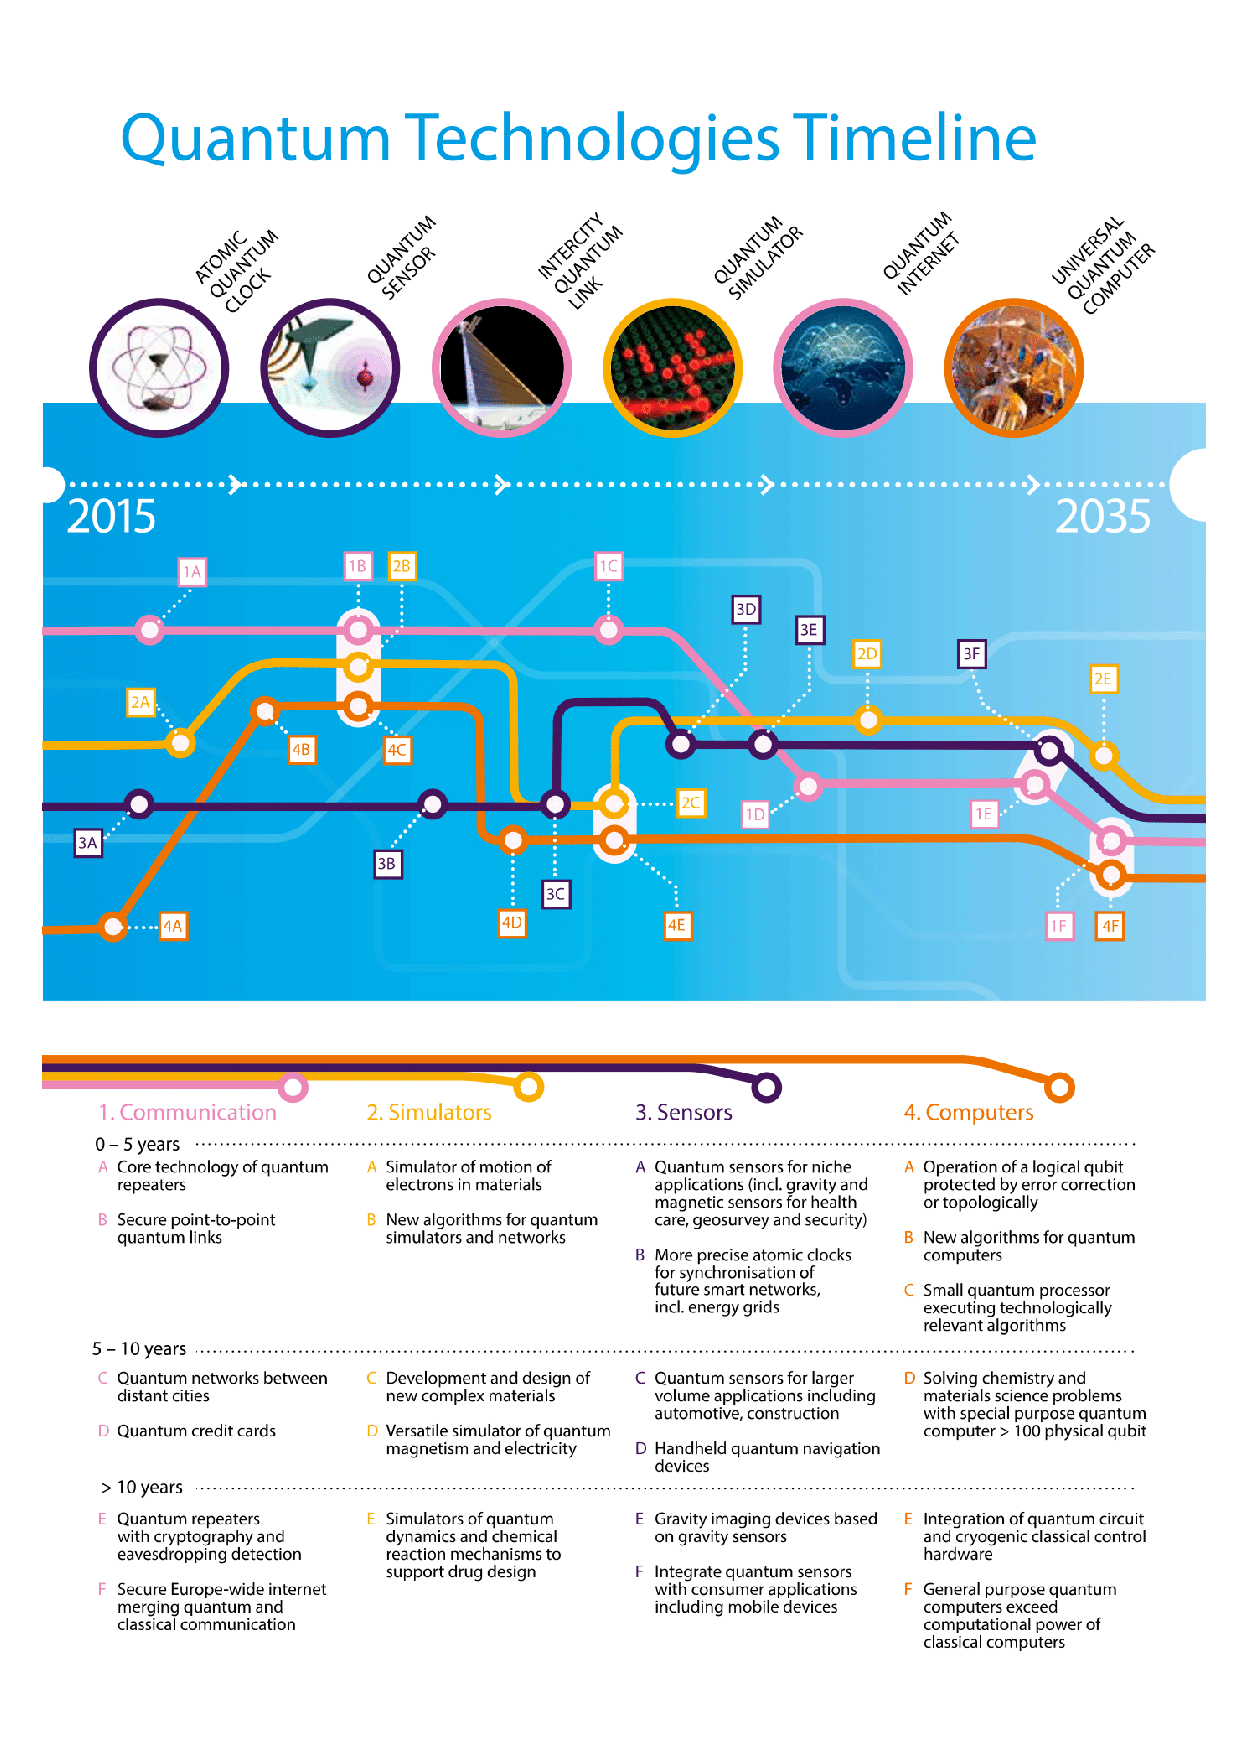
\includepdf{kep.pdf}
A kutatási, fejlesztési célokon felül egy igen fontos terület még az elméleti eredmények gyakorlatba ültetése, a mindennapi életet segítő piacképes alkalmazások létrehozása, aminek fő eszköze az ipar. Ennek a fontossága a Manifesto-ban is látszik hiszen a vezető kutatási szerepen túl megjelölt a legfontosabb cél egy növekvő és versenyképes európai iparnak kedvező körnezet kialakítása. A kvantumkommunikáció terén a technológia fejlődésével az elmúlt években a kutató intézeteken kívül szerencsére egyre több ipari szereplő is elkezdett foglalkozni, mind európában, mind világszerte, ami az egyre közeledő széleskörűbb gyakorlati alkalmazások elterjedését jósolhatja. Ezekről egy kis áttekintő: \\

\section*{Kvantumkommunikációval foglalkozó cégek}

Az Európában kvantum technológiához köthető vállalkozásokról található egy adatbázis a QUROPE oldalán: \url{http://qurope.eu/db/industries} . A kvantumkommunikációhoz valamilyen módon köthetó vállalkozások nagy része egyelőre főprofilként hagyományos optikával(pl.:Adva Optical Newtorking,ADVR,Corning) valamint hagyományos IT biztonsági megoldásokkal(pl.:Eleven Paths,Genua,Omnisec,Senetas) foglalkozik, konkrét kvantumos megvalósításokkal nem. A főprofilként kvantumos technológiákkal foglalkozó fiatalabb cégek viszont terjednek, ilyenek például az ID Quantique SA, QuTools, SeQureNet és SQR Technologies.\\
\underline{ID Quantique SA}  (\url{http://www.idquantique.com/}) 
\includegraphics[height=0.5cm, keepaspectratio]{idq.png}\\
Az ID Quantique SA egy svájci vállalat, az itt felsoroltak közül a legnagyobb múlttal rendelkező, 2001 óta foglalkozik QKD megvalósításokkal és kínál is megoldásokat a piac számára. A kulcsszétosztáson kívül, mára már kvantum véletlenszám generátorokkal is bővült a kínálata. A világon jelenleg működö QKD hálózatok közül több kiépítésében is szerepet vállalt(pl.: Svájci, Tokiói QKD hálózat)\\
\underline{QuTools} (\url{http://www.qutools.com/}) 
\includegraphics[height=0.5cm, keepaspectratio]{qutools.png}\\
A QuTools egy 2005-ben alapított német cég, különböző kvantumkommunikációs technológiákban használatos eszközökkel foglalkozik. Kínálatukban találhatók kvantumos fotondetektorok és generátorok, valamint véletlenszám generátorok is.\\
\underline{SeQureNet} (\url{https://www.sequrenet.com/}) 
\includegraphics[height=0.5cm, keepaspectratio]{sequrenet.png}\\
A SeQureNet egy 2008-ban alapított francia startup, CVQKD(Continuous Variable Quantum Key Distribution) megvalósítást kínál a piac számára, amibe beletartozik mind az ehhez tartozó hardver és a hozzá tartozó szoftver is.\\
\underline{SQR Technologies} (\url{http://www.sqrtech.com/}) 
\includegraphics[height=0.5cm, keepaspectratio]{sqr.png}\\
Az SQR Technologies 2010-ben alakult Belgiumban,jelenleg ultragyors véletlenszám generátorokat( ~4Gbps) kínálnak és fejlesztenek.\\

A célzottan kvantumkommunikációval foglalkozó vállalkozásokon kívül nagyobb ipari szereplők közül is vannak a témában erősebb érdekeltséggel rendelkezők Európában. Angliában a British Telecom és a Toshiba ottani kutatólaboratóriuma dolgozik kvantumkommunikciós technológiák megvalósításán.Rajtuk kívül ilyen még például az Atos akiknek van egy átfogóbb kvantumos programjuk, melyben a kvantumkommunikáción belül a kvantumkriptográfiai algoritmusok fejlesztése is szerepet kapott.A holland KPN a már korábban említett ID Quantique -val közösen pedig a hálózatán tesztelt QKD-t.\\
Az Európai szereplőkönt kívül természetesen világszerte egyre több vállalat foglalkozik kvantumkommunikációval, köztük már ismertebb nagyobb multú, akár multinaciónális cégek is. Az AT\&T és Caltech(California Institute of Technology) kvantumhálózatok fejlesztésén dolgozik, a Raytheon QKD megvalósítás után lehetséges kvantum ismétlő fejlesztésével foglalkozik, kvantum kriptográfia és kommunikáció szerepel a HP érdekeltségi listáján is, az SK Telecomnak is van már kvantumkommunikációs részlege, valamint Japánban a Tokiói QKD hálózatban együttműködő partnerek között ott van a NEC, Mitsubishi és NTT(Nippon Telegraph and Telephone), valamint a 2015-ös akkori QKD távolságrekord felállításában partner volt a Fujitsu is.\\
A főprofilban kvantumkommunikációval foglalkozó cégek közül a korábban már említetteken túl  piackész rendszererekkel rendelkezik az ISARA (aki kvantumos kutatásban együttműködik a Blackberryvel, szakterültetük a poszt-kvantum kriptográfia), MagiQ (kvantumkriptográfiai rendszer, összefonódott fotonpár forrás), NuCrypt (Összefonódott fotonpár forrás és detektor), QuantumCTek (QKD rendszerek, források, detektorok), Qubitekk (QKD rendszer), Quintessence Labs (véletlenszám generátor, biztonsági megoldások) és UQDevices (detektor). Ezeken a vállakozásokon felül vannak még egyelőre termék nélküli kutatás fejlesztéssel, valamint tanácsadással foglalkozók is. A Wikipédián a teljesség igénye nélkül található egy lista a témában érdekelt vállalatokról ami kiindulási alapként szolgálhat: \url{https://en.wikipedia.org/wiki/List_of_Companies_involved_in_Quantum_Computing_or_Communication}.





%\clearpage

A LaTex nyelv elsajátítása, irodalomkutatás, valamint a dokomentum írása megközelítőleg két és fél hetet vett igénybe, az ezutáni néhány napban, pedig a konzultációk utáni kisebb változtatások,javallatok, kérések eszközlésével foglalkoztam, majd véglegesnek minősítettük az eredményt.

\subsection *{Prezentációt segítő anyagok}

A gyakorlat második felében a cél olyan később is felhasználható anyagok készítése volt, amik a kvantumkommunikáció, valamint annak mára már egyre növekvő ipari jelenlétének bemutatására használhatóak. Kiindulópontnak egy a kvantumkommunikáció fejlődését bemutató timeline, valamint egy a jelenlegi kvantumkommunikációs ipari helyzetet leíró térképet határoztunk meg célnak.\\ 
A munkámat a timeline elkészítésével kezdtem, mivel az ide gyűjtendő információkból rendelkeztem egy kevés előismerettel. Ennek következtében arról is volt egy pontosabb elképzelésem, hogy mi kerülhet majd a végtermékre. Az elkészüléshez szükséges idő nagy részét ebben az esetben is az irodalomkutatás vette el.  Véleményem szerint ez a kvantumos technológiák fiatalságának, valamint, annak, hogy ezen belül is a viszgálandó terület igen specifikus és szük volt. Ennek következtében a felhasználható források maguk is igencsak szűkösek voltak. A kezdeti évekhez hasznos forrásnak bizonyultak az akkoriban publikált témába vágó kutatások. Ezeknak a hátránya volt viszon, hogy bennük egy specifikus információ keresése igen nehézkes, sok esetben szükséges hozzá az egész dokumentum elolvasása.Ezekhez a részekhez azt a stratégiát alkalmaztam, hogy néhány jól megválasztott kulcsszóval a szűkebb témát ki tudtam szűrni a találatok közül(Google Scholar), majd a keresési idősáv egy évre történő leszűkítésével megkaptam az éppen aktuális évhez tartozó elolvasandó publikációkat. Ezen felül használtam még az olvasott publikációkban található hivatkozásokat is, hogy megtaláljam azt, ami fölött a fenti módszerrel esetlegesen átsiklanék. Az időben  későbbi adatok nagyrésze már nem feltétlen tudományos lapokban publikált kutatási eredmény volt, hanem a területen alakuló ipar eredményei. Itt az előző taktikát értelemszerűen már nem lehetett használni. Az említett adatok túlnyomóan cikkekből, azokban található hivatkozásokból származnak. A kész ábrával kapcsolatban elvárás volt, hogy vektorgrafikus legyen, ezért a Microsoft Visio program segítségével készítettem.\\
Az elkszült ábra.
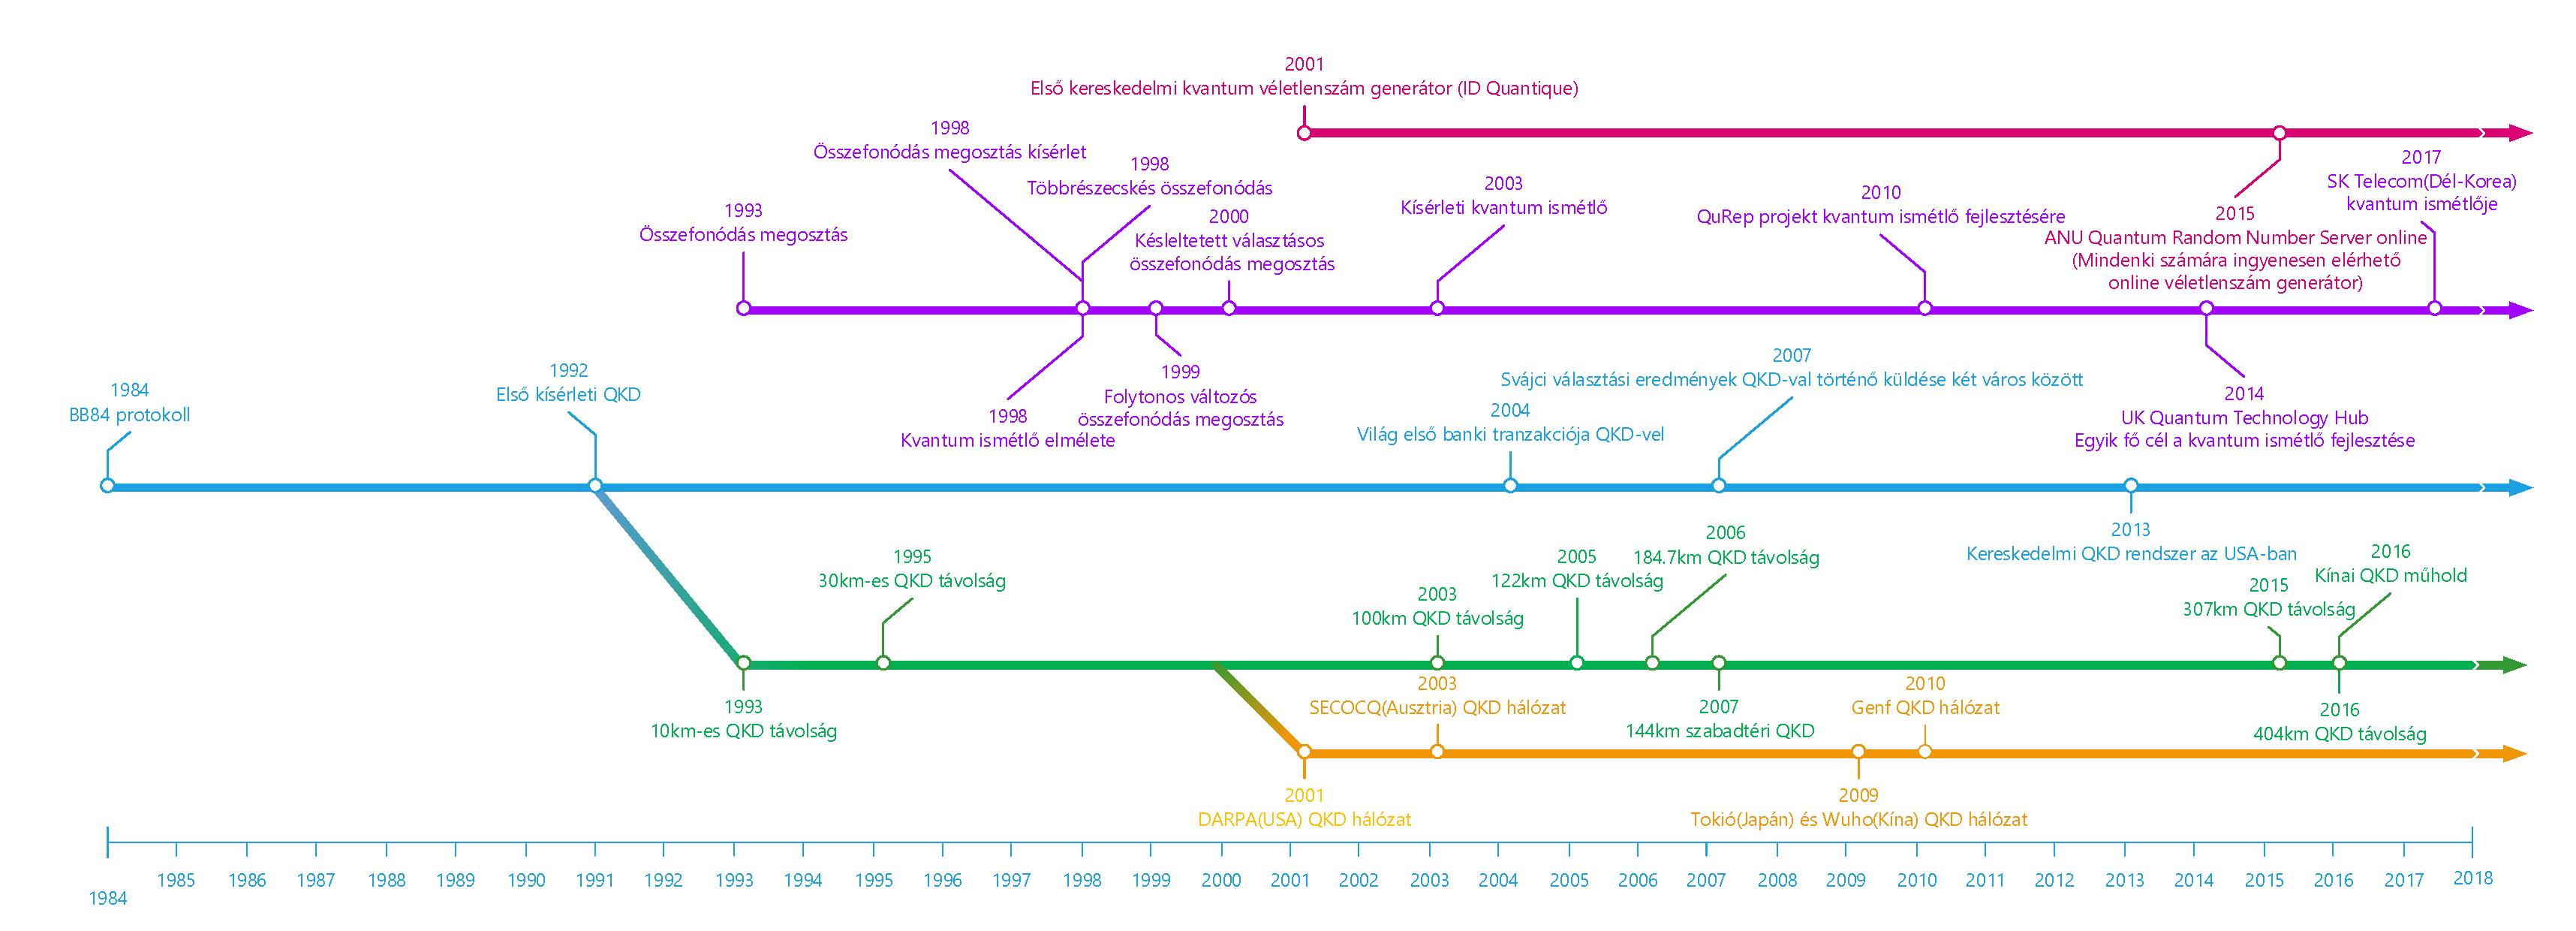
\includepdf{timeline}
A második feladatban kezdetben a cél egy világtérkép elkészítése volt az ipari szereplők feltüntetésére, amin a kvantumkommunikációs fejlesztéshez kapott támogatás/képviselt érték szerint lehetett volna színezni. Ezen sajnos a rendelkezére álló információk hiánya miatt részben változtatni kellet. Ennek megfelelően az ehhez tartozó irodalomkutatás jelentősebb része ennek kiderítésével telt. Itt nagyban mutatkozott a terület fiatalsága, valamint az ebből származó hátrányok a gyűjtés szempontjából. A legtöbb kizárólag témakörrel foglalkozó ipari szereplőről még nem találhatóak felmérések, cikkek. A nagyobb piaci szereplőkről pedig akik a témában kutatnak kisebb, nagyobb csoportokkal, részlegekkel, a technológiát hasznosító késztermék hiányában nincs olyan gazdasági említés, amiben ez a kis részleg/csoport kezelhető számokkal külön említésre kerülne.Használható kimutatást a témához összesen egyet találtam, körülbelül 1500 dollárért, emiatt a későbbi konzultáció után úgy döntöttünk, hogy a feladatott módosítjuk. Az új elkészítendő térkép ezek alapján bejegyzett kvantumkommunikációs cégekkel rendelkező országok szemléltetésére szolgál. Ehhez az előzővel ellentétben, habár még mindig nehézkesen, de már lehetett elégséges mennyiségű információt találni. Ehhez az ábrához is természetesen elvárás volt a vektorgrafikusság. Az összegyűjtött anyagok és az Adobe Illustrator program segítségével készült el végül az alábbi ábra:\\
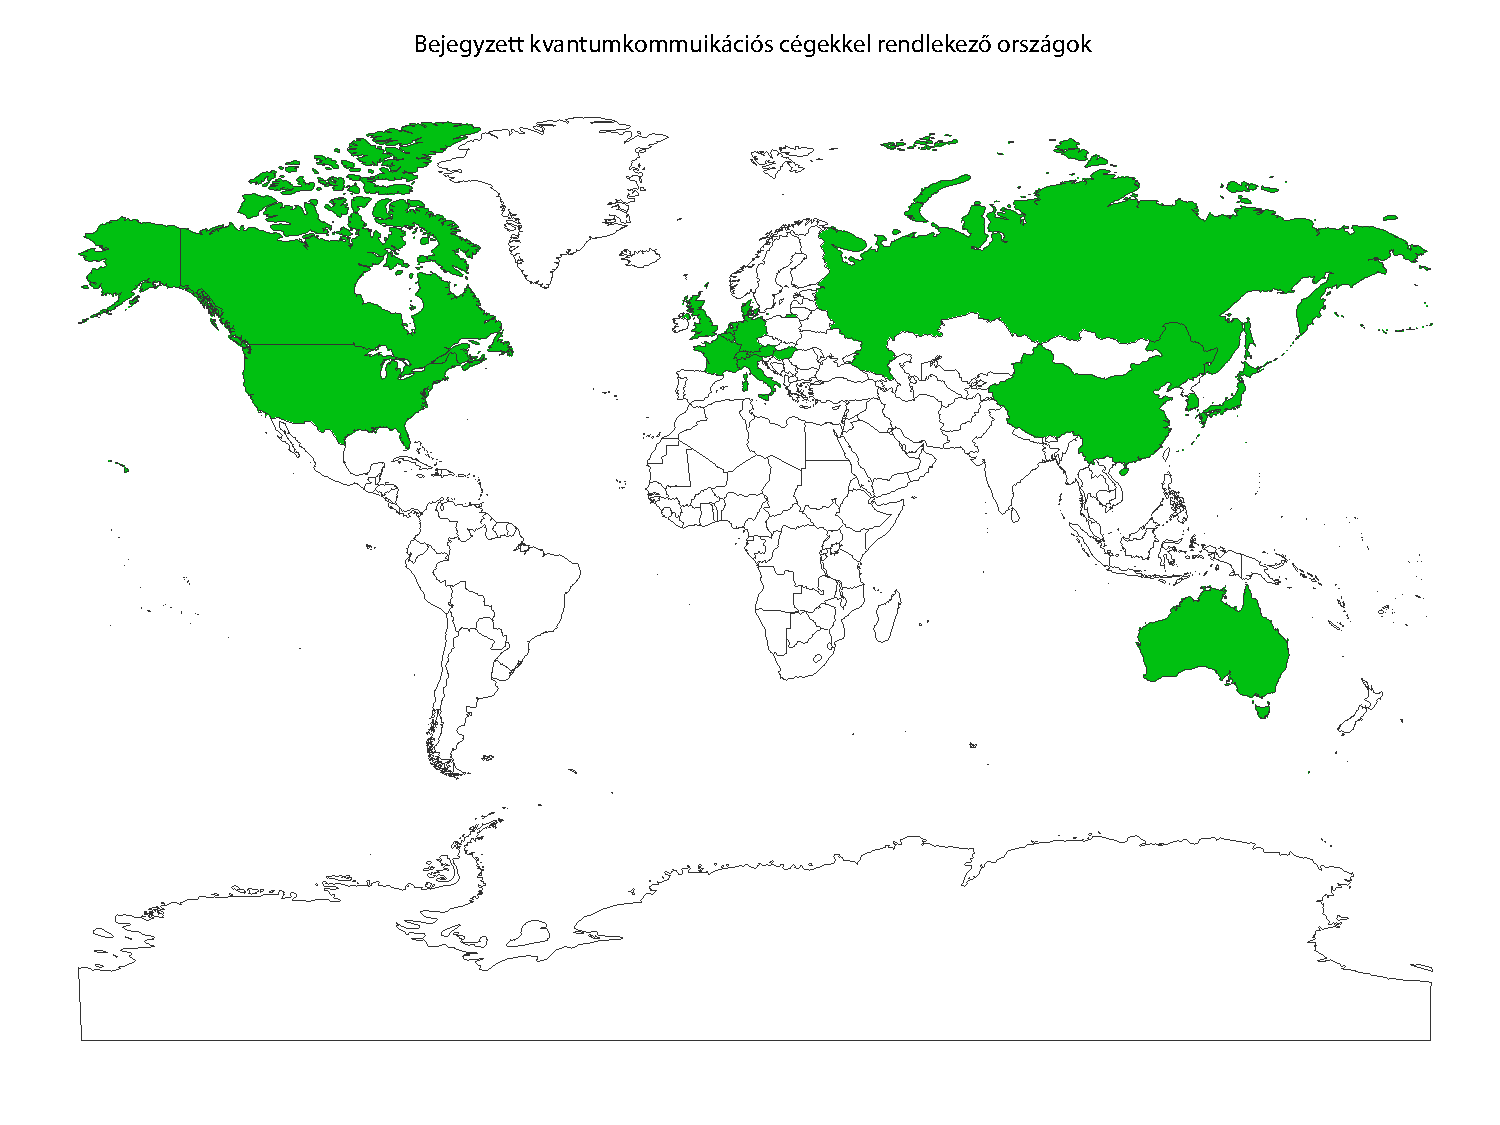
\includepdf{terkep}
Ezek után egy lehetséges plakát tervén kezdtem el dolgozni. Ennek témául a kvantumkommunikáció mint terület, valamint a kvantumismétlők, mint itteni előrelépési lehetőség rövid bemutatását tűztük ki célul. Ehhez a fentieken túl szükséges volt még néhány magyarázó ábra elkészítése, valamint a plakátra kerülendő szöveg megírása. Design tapasztalattal sajnos nem rendelkeztem,  kezdetben az így megalkotott anyagokból (timeline, térkép, ábrák, szöveg) próbáltam az Illustrator segítségével elfogadható plakátot varázsolni. Ekkorra már közeledett a gyakorlat vége, egy plakáttervvel el is készültem, viszont tudván, hogy megfelelő tapasztalattal szebbet és jobbat tudnék, megkérdeztem a konzulensem arról a lehetőségről, hogy a gyakorlat végeztével felkeresem egy ilyen témában jártasabb ismerősöm segítségért a plakát kinézetéhez. Ő készítette a következő tervet:\\
\includepdf{project}
A plakáton látható ábrák, valamint szövegek a gyakorlatom végének termékei, az elrendezés és design már a tapasztaltabb ismerősöm érdeme. A cím értelemszerűen placeholder szerepet tölt be. A design véglegeítését valószínüleg szeptember hónapban tudom befejezni, mivel ekkorra tudtunk csak találkozót megbeszélni az ismerősömmel aki a megjelenéstervet készítette.(Ez szükséges, mivel az általa a tervezéshez használt eszközöket én magam nem ismerem kellően) A tervet azóta a gyakorlatom rendezői is koncepciójában elfogadták, a talákozón már csak véglegesítés és rövid közös kidolgozás várható. Emiatt a most ismertetett koncepció a plakát végleges kinézetét, valamint elrendezését tekintve mérvadónak tekinthető.\\
\section*{Összefoglalás}
A gyakorlat során sok olyan tudást szereztem amit egyetemi tanulmányaim során eddig nem, egy már korábban tanulmányozott témát közelíthetttem meg egy új szemszögből. Az elvégzett feladatok, valamint az ezek során fellépő nehézségek rávilágítottak számomra arra, hogy egy-egy téma, munka, technológia elérhetősége mennyire sokat is számít, valamint, hogy ennek hiánya mekkora hátrányt jelenthet számára.


\chapter{Bevezetés}

\section{Motiváció}

A számítógépes rendszerek elterjedésének természtes következménye volt az őket összekötő hálózatok megjelenése és fejlődése. Napjainkban egyre kevesebb olyan eszközt találni, amely ne lenne alkalmas egy ilyen hálózatra való csatlakozásra, rengetek alkalmazás és funkció van, ami valamilyen hálózatból kapott információra támaszkodik működése során. Tekintve a kvantummechanikára építő technológiai megoldások fejlődését, kísérleti kvantumszámítógépek jelenlegi állását\cite{IBMQC}\cite{neill2017blueprint} , az ilyen kvantumos erőforrásokat használó eszközök összekötésére alkalmas hálózatokra is igény lesz. További motivációt jelent még, hogy ezen kvantumos információ továbbítására alkalmas hálózatok sok más felhasználási lehetőséget kínálnak a leendő kvantumszámítógépek összekapcsolásán túl. Ezek közül talán a legismertebb és legelterjedtebb a kvantum kulcsszétosztás, ahol kvantumos állapotokat használunk titkosított kulcsok bizonyítottan biztonságos megosztására.\cite{BB84} Ezt a technológiát már a valós életben is használják, nem csak kutatási célokra.\cite{Swisselection} Mindezek hatására egyre nő az egyre nagyobb ilyen hálózatokra való igény, egy jövőbeli kvantum internet\cite{kimble2008quantum} megvalósítára való törekvés. Ennek jelenleg a legnagyobb gátat a távolság jelenti. A klasszikus információval ellentétben a kvantumos infromáció nem másolható \cite{wootters1982single}, emiatt a klasszikushoz hasonló erősítők sem alkalmazhatóak a kommunikációs csatorna által okozott veszteségek korrigálására. Ezt leküzdendő születtek meg különböző megvalósítások, az egyik ilyenek egy csoportja az ún. kvantum ismétlők. Itt a fő cél a küldő és a fogadő állomás között összefonódott párok megosztása. Ezután az összefonódás különös tulajdonságait felhasználva a felek már különböző kvantumos műveletekre képesek. Tetszőleges kvantumbit küldése például a párok és egy klasszikus kommunikációs csatorna valamint a kvantum teleportációs protokoll\cite{bennett1993teleporting} segítségével már megvalósítható. A kvantum ismétlő protokollok ugyan működésük kvantumos alapokon nyugszik, a velük kapcsolatos megoldandó problémák jelentős része hasonlít a klasszikus hálózatokban felmerülőkhöz. Ezen protokollok hatékony megvalósításhoz is szükséges több elosztott erőforrás megfelelő együttműködése, itt is fontos szerepet kap példul a hibakezelés, vagy éppen az adott lépések megfelelően összehangolt végrehajtási sorrendje. 

\section{Feladatkiírás}
A feladatkiírás négy főbb pontot jelöl meg a dolgozat témáját tekintve, a következőképpen:\\
(\textit{idézve a feladatkiírásból})\\

A hallgató feladatának a következőkre kell kiterjednie:
\begin{itemize}
\item A kapcsolódó szakirodalom áttekintésével mutassa be a kvantum alapú informatikát és
kvantum alapú kommunikációt!
\item Mutassa be részletesen az összefonódás megosztásának elvét és ismertesse a különböző
felhasználási lehetőségeket, valamint technológiai megoldásokat!
\item Válasszon alkalmas szoftverkörnyezetet és készítsen szimulációt az összefonódás
megosztásának lehetőségeinek vizsgálatára kvantum alapú vezetékes és vezeték nélküli
hálózatokban!
\item Értékelje a kapott eredményeket!
\end{itemize}
Ennek megfelelően a dolgozatot egy gyors történeti áttekintés, majd egy hosszabb elméleti bevezető nyitja. Ezek után a készített szimuláció leírása, majd végül a szimulációs eredmények és ezeken keresztül egyes technológiai megvalósítási lehetőségek áttekintésével zárul.




%---%
\chapter{Áttekintés}
%---%

\section{A kvantumkommunikáció napjainkig}

A kvantumkommunikációról valamint kvantuminformatikáról mint kutatási területről, valamikor a 90-es évek eleje-közepe óta beszélhetünk, habár az általa vizsgált és használt főbb jelenségekkel a fizika már az 1920-as években is foglalkozott. Elég csak azt tekinteni, hogy a kvantummechanika egyik mai meghatározó alapköve az 1926-ban publikált Schrödinger-egyenlet \cite{schrodinger1926undulatory}. Az azóta eltelt időben a témához kapcsolható talán leghíresebb történés az 1980-as évekig az 1935-ös ún. EPR-paradoxon \cite{einstein1935can} valamint ennek kapcsán Bell 1964-es válasza \cite{bellt1964einstein}. Az EPR-paradoxonban Einsteinék összefonódott párok azon különleges tulajdonságát vizsgálták, hogy az egyik részecskén elvégzett véletlen eredményű mérés hatással van az összefonódott pár másik tagjára is, távolságtól függetlenül.  Mivel az azonnali információterjedés lehetősége a relativitáselméletben megismertekkel ellenkezik, helyi, rejtett, számunkra ismeretlen változók ötletével álltak elő ennek magyarázatára. Így ezekbe az ismeretlen változókba lehetséges lehetne előre eltárolni információt, ami alapján a számunkra véletlennek tűnő méréseknél a pár mégis korreláló eredményeket mutathat. Mivel a kvantummechanikában ilyen rejtett változók nincsenek, ezért szerintük a kvantummechanikának hiányosnak kellett lennie. Bell 1964-es írásában erre reflektál. Az általa levezetett egyenlőtlenség lehetővé tette ezen elméletek kísérleti tesztelését, melyek később a kvantummechanika jóslatait igazolták, a rejtett változós elképzeléssel szemben.\\
 Az 1980-as években már kezdték vizsgálni ezen jelenségek későbbi lehetséges alkalmazásait, 1982-ben született a később meghatározó ``No Cloning Theorem'' \cite{wootters1982single}, ami a tetszőleges kvantumbit másolhatatlanságát mondja ki, továbbá 1984-ben merült fel az első kvantumkriptográfia protokoll ötlete is \cite{BB84}. Az 1990-es évektől kezdődően pedig kísérleti megvalósításokkal is találkozhatunk. További meghatározó eljárások születtek, mint például a kvantum teleportációs protokoll \cite{bennett1993teleporting}, majd ennek későbbi kísérleti megvalósítása \cite{bouwmeester1997experimental}, vagy akár az elméletben RSA titkosítás törésére is használható Shor-algoritmus \cite{shor1999polynomial}. Kvantumkommunikációs szempontból 1992-ben először hajtottak végre sikerrel kvantum kulcsszétosztást \cite{bennett1992experimental}, valamint 1993-ban felmerült az összefonódás megosztás ötlete \cite{zukowski1993event}, amit 1998-ban kísérletileg is megvalósítottak \cite{pan1998experimental}. Fontos előrelépés volt még az első összefonódás tisztító eljárások \cite{bennett1996purification}\cite{deutsch1996quantum} megjelenése is, később ezen újítások segítségével vázolták fel a kvantum ismétlő ötletét \cite{briegel1998quantum}. \\
 Az elkövetkezendő években egyre hatékonyabb eljárások, valamint az új technológiák segítségével pontosabb és megbízhatóbb kísérletek készültek. Ezt bizonyítja, hogy a 2000-es évek közepétől kezdtek elérhetővé válni (főleg kvantumkriptográfiában) a nagyközönség számára is használható kvantumos termékek. A folyamatos fejlődés megfigyelhető a kapcsolódó kutatások növekedésén is, idővel egyre több helyen alakultak a témába vágó kutatóközpontok, valamint kísérleti kvantumhálózatok. Egyre közeledünk az előzetes kutatások iparban való felhasználhatóságához. Ezt mutatják a közelmúltban a témában elért eredmények is. Ezek közül az egyik talán legjelentősebb a kínaiak által 2016-ban Föld körüli pályára állított műhold \cite{chinasat} kvantum kulcsszétosztás tesztelésére, melyről már kísérleti eredmények is származnak \cite{yin2017satellite}. Megemlítendő még, hogy felismerve a területben rejlő lehetőségeket, a kvantumos kutatások támogatása bekerült az Európai Unió fejlesztési tervébe is, amely keretében 1 milliárd euró értékben támogatnak kvantumtechnológiai kutatásokat és fejlesztéseket \cite{manifesto}.\\
 \begin{figure}[h]
\centering
\makebox[\textwidth][c]{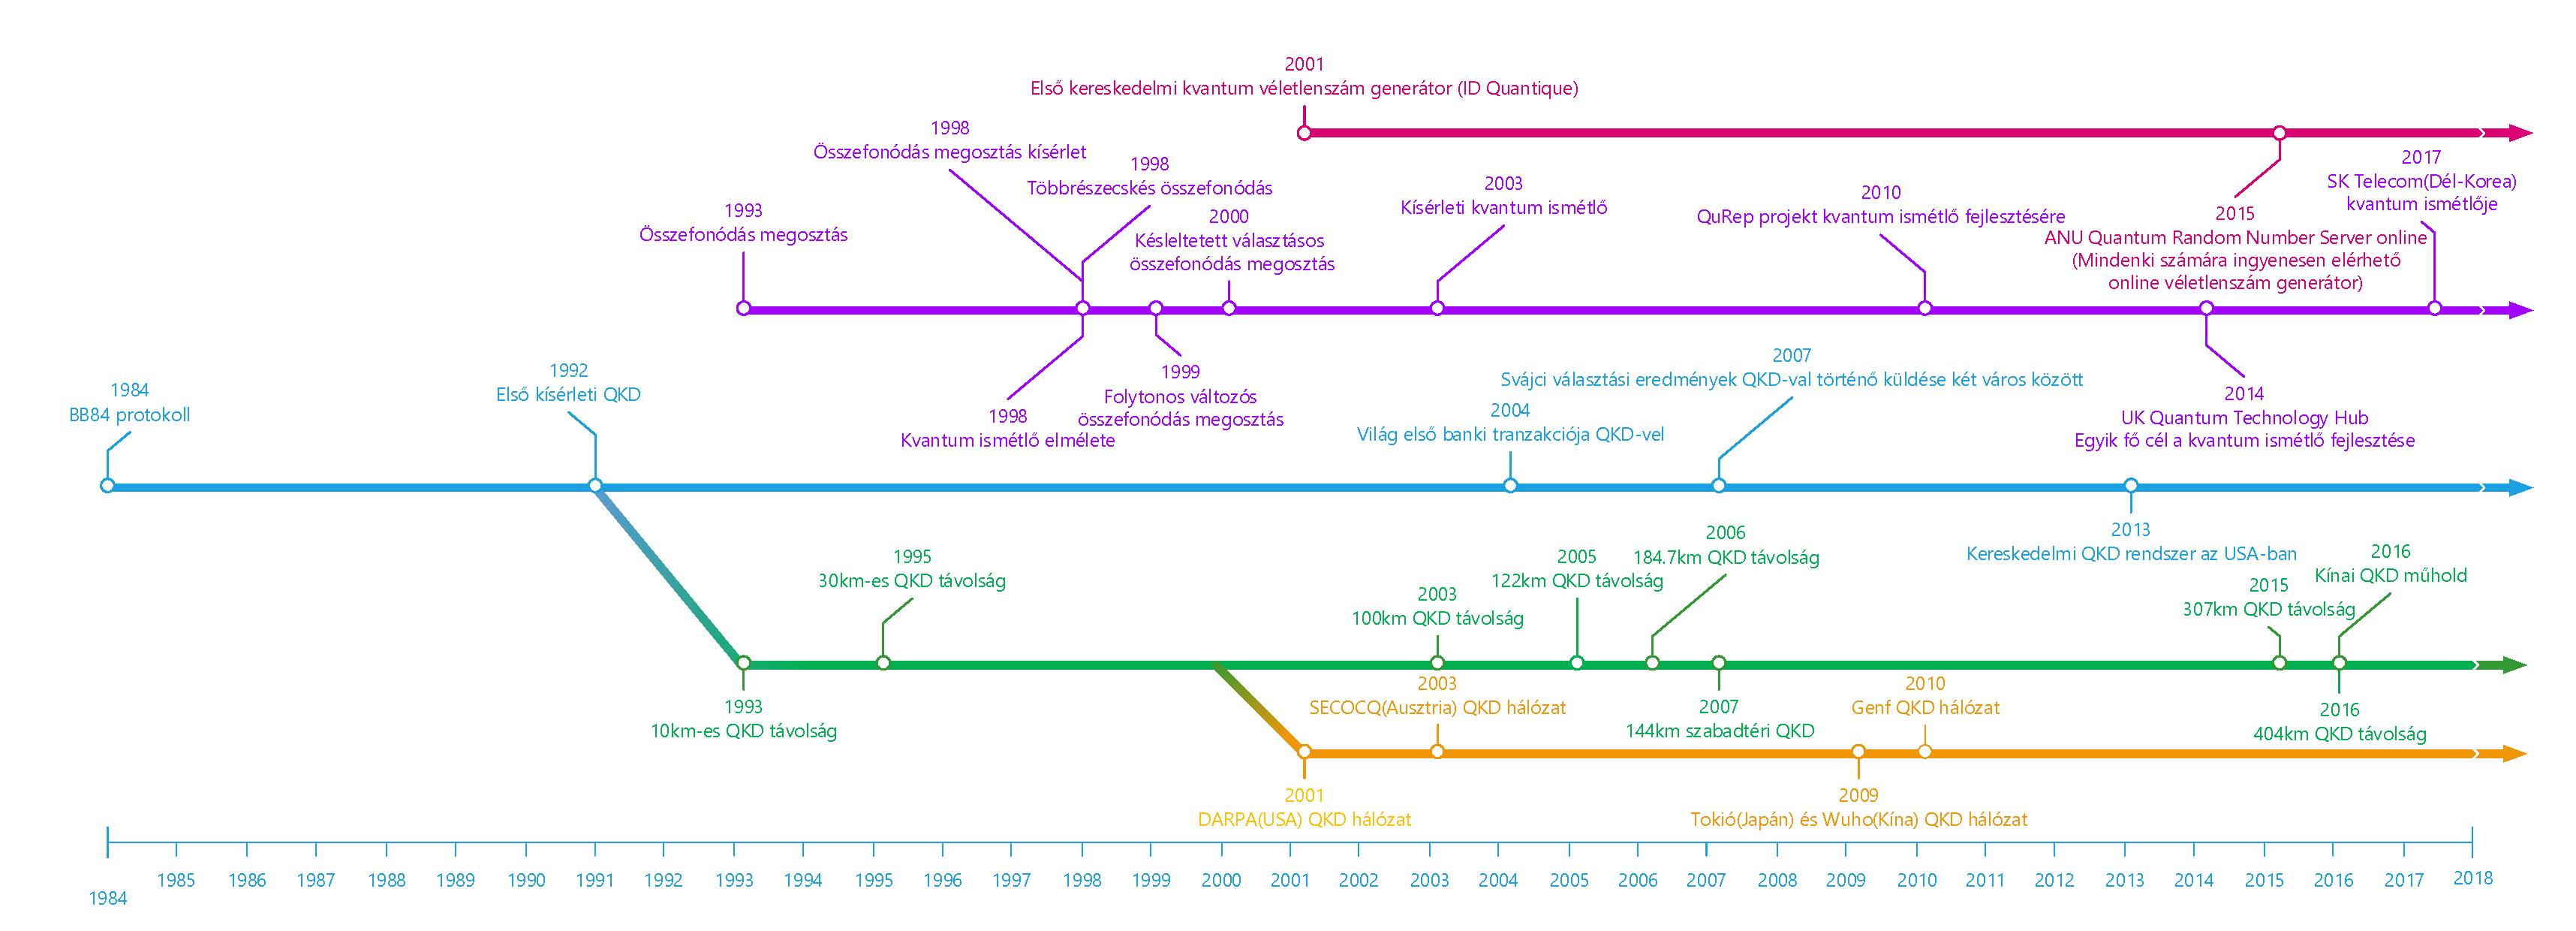
\includegraphics[height=\textheight]{timeline}}
\caption[Kvantumkommunikáció timeline]{Kvantumkommunikáció fejlődése 1984-től}
\end{figure}
A ``kvantum internet'' \cite{kimble2008quantum}\cite{pirandola2016unite} megvalósításához azonban még mindig le kell küzdeni a hozzáférési pontok közti távolságból adódó problémákat. Habár a kapcsolódó technológiák fokozatosan javultak az évek során, olyan megbízható, hibatűrő rendszer ami ehhez kéne még nincs. A közeljövőben erre két kutatási terület is kínálhat megoldást: egyes kvantum hibajavító kódok \cite{lidar2013quantum} melyek alkalmazhatóak hálózatokra is \cite{zhang2013quantum}, valamint a kvantum ismétlők\cite{uphoff2016integrated}\cite{krovi2016practical}\cite{pfister2016quantum}\cite{li2016heralded}. A dolgozat a továbbiakban ezek közül a kvantum ismétlőkkel foglalkozik. 






%---%
\chapter{Elméleti Bevezető}
%---%

\section{Elméleti alapok}

\subsection{Posztulátumok: \cite{kvantkonyv1}} 
\underline{1.állapotteres leírás:} Egy zárt fizikai rendszer éppen aktuális állapota leírható egy \textbf{V} Hilbert tér-beli egységhosszú, komplex együtthatós állapotvektorral. Hilbert tér például egy komplex lineáris vektortér, amire értelmezve van a belső szorzat(skalárszorzat). 
Vegyünk példának egy két dimenziós Hilbert teret, ami egy egyszerű zárt fizikai rendszer jelképez. A rendszer állapotát le lehet írni egy /textbf{v} két dimenziós vektorral, ahol:\\
\begin{center}
$ v= \begin{bmatrix} a\\b \end{bmatrix} = a\textbf{0}+ b\textbf{1} $ ,ahol 
$\textbf{0}=\begin{bmatrix} 1\\0 \end{bmatrix} , \textbf{1}=\begin{bmatrix} 0\\1 \end{bmatrix} ,   a,b \in C$
\end{center}
Itt \textbf{0} és \textbf{1} az orthonormális(ortgonális és egyséhosszú) bázisvektorok. Mivel az állapotvektor egységhosszú,ezért ki kell még kötni, hogy 
$\abs{a}^2+\abs{b}^2 =1$ . Az együtthatókra szokás még valószínűségi amplitúdóként is hivatkozni(a Schrödinger hullámfüggvényben amplitúdóként jelennek meg).

\underline{2.Rendszerek időbeli fejlődése:}Zárt fizikai rendszer időbeli fejlődése leírható csak változás kezdő- és végpontjától függő unitér transzformációval. Az előbbi jelölésrendszer segítségével leírva: 
\begin{center}
$v'(t_2) = U(t_1,t_2)v(t_2), v' \in V$
\end{center}
$ U $ unitér operátor lineáris algebrai reprezentációja egy \textbf{U} kvadratikus mátrix, melynek $U_{ij}$ elemei a bemeneti \textbf{j} orthonormális bázisvektor \textbf{i} vektorral való kapcsolatát jelképező valószínűségi amplitúdókat jelölik.\\

\underline{3.Mérés:} Méréseket leírhatunk$M_m$  mérési operátorokkal, ahol $m$ a lehetséges mérési eredményeket jelöli. $m$ mérésének a valószínűsége, ha a rendszer \textbf{v} állapotban van:
\begin{center}
$P(m|\textbf{v})= {\textbf{v}}^\dagger M_m^\dagger M_m \textbf{v} $
\end{center}
A rendszer állapota mérés után:
\begin{center}
$ {\textbf{v}}' = \frac{M_m \textbf{v}}{\sqrt{{\textbf{v}}^\dagger M_m^\dagger M_m \textbf{v}}}  $
\end{center}
Mivel a kimenetek összesített valószínűsége 1-el egyenlő.(a lehetséges kimenetek lefedik a teljes eseményteret):
\begin{center}
$ \sum_m P(m|\textbf{v}) = \sum_m {\textbf{v}}^\dagger M_m^\dagger M_m \textbf{v} \equiv 1$
\end{center}
ami alapján:
\begin{center}
$\sum_m M_m^\dagger M_m \equiv I $
\end{center}
A mérések nem visszafordíthatóak és viszonylag durvának tekinthetőek abból a szempontból, hogy befolyásolják a mért rendszer állapotát a fentebb már leírt módon. Ugyanakkor velük teremthetjük meg a kapcsolatot a klasszikus és a kvantum világ között, mivel ők azok az eszközök,  amikkel megfigyelhetjük mégiscsak mi történik a kvantum világban.
\\
\underline{4.Összetett rendszerek:}
Egy $ W $ összetett fizikai rendszer állapota leírható az őt összetevő rendszerek tenzorszorzataként:
$ W=V \otimes Y $ .Továbbá ha $\textbf{v} \in V  $  és  $ \textbf{y} \in Y $ akkor a belőlük alkotott állapot: $ \textbf{w}=\textbf{v}\otimes \textbf{y} $ .
A kvantummechanikában a legkisebb információt hordozó elem a bit, amit kvantumbitnek, vagy röviden qubitnek  szokás hívni. Egy qubit szokványos leírása:
\begin{center}
$ \ket{\psi}=a\ket{0}+b\ket{1}=a \begin{bmatrix}1\\0\end{bmatrix}+ b \begin{bmatrix}0\\1\end{bmatrix} = \begin{bmatrix} a\\b \end{bmatrix} $
\end{center}
A klasszikus számítástechnikához hasonlóan n qubit felhasználásával építhetünk n bites kvantumregisztereket. Vizsgáljunk például egy két qubitből alkotott kvantumregisztert. Ekkor a teljes két qubites rendszer állapota:
\begin{center}
$ \ket{\psi} \equiv \ket{\psi_1}\ket{\psi_2} \equiv \ket{\psi_1,\psi_2} \equiv \ket{\psi_1\psi_2} $
\end{center}
Ami például hogyha:
\begin{center}
$ \ket{\psi_1} = \frac{\ket{0}+\ket{1}}{\sqrt{2}}, \ket{\psi_2}=\frac{\ket{0}+\ket{1}}{\sqrt{2}}, $
\end{center}
akkor:
\begin{center}
$ \ket{\psi}= \frac{\ket{0} \otimes \ket{0} +\ket{0}\otimes\ket{1}+\ket{1}\otimes\ket{0}+\ket{1}\otimes\ket{1}  }{2} = \frac{\ket{00}+\ket{01}+\ket{10}+\ket{11}}{2} $
\end{center}
látszik, hogy az előbbi rendszer a 00,01,10,11 állapotok(ők mellesleg ortogonálisak egymásra,itt az állapottér bázisának tekinthetőek) súlyozott(most itt mindegyik 1/2 -el de ez lehet bármilyen más komplex szám is, sőt akár 0 is.) összege, ezeket mind tartalmazza és jól látszik, hogy felbontható $\ket{\psi_1}$  és  $\ket{\psi_2}$  tenzorszorzatára. Az ilyen állapotokat hívjuk szorzat állapotoknak.\\
Most vizsgáljuk a következő állapotot:
\begin{center}
$ \ket{\psi} = a\ket{00}+b\ket{11} $
\end{center}
Ezt nem tudjuk felbontani két qubit tenzorszorzatára. Az ilyen állapotokat hívjuk összefonódott állapotnak. Vegyük észre ennek az állapotnak egy érdekes tulajdonságát. Ha megmérjük az egyik bitjét, akkor akkor valamilyen valószínűséggel 0-át vagy 1-et kapunk. Viszont ha ezután megmérjük a másik bitet is, ha az első mérésünk eredménye 0 volt, akkor itt már csak 0 mérhetünk és ehhez hasonlóan 1-es eredmény esetén pedig csak 1-et. Továbbá kísérletileg bizonyított, hogy ez a jelenség akkor is fenn marad, ha a rendszer két qubitjét helyileg egymástól eltávolítjuk.
Néhány nevezetes összefonódott állapot, amelyeket Bell-állapotoknak szokás nevezni:
\begin{center}
$ \ket{\Phi^-}= \frac{1}{\sqrt{2}}(\ket{0_A0_B}-\ket{1_A1_A}) $ \\
$ \ket{\Phi^+}= \frac{1}{\sqrt{2}}(\ket{0_A0_B}+\ket{1_A1_A}) $ \\
$ \ket{\Psi^-}= \frac{1}{\sqrt{2}}(\ket{0_A1_B}-\ket{1_A0_A}) $ \\
$ \ket{\Psi^+}= \frac{1}{\sqrt{2}}(\ket{0_A1_B}+\ket{1_A0_A}) $ \\

\end{center}

Figyeljük meg, hogy ezek az állapotok egymásra merőlegesek, az állapotérnek bázisaiként szolgálhatnak. Ennek segítségével definiálhatjuk az ún. Bell mérést ami egy 2 qubites rendszer projektív mérése ezekben a bázisokban. Megjegyzendő még, hogy a mérés után a mérési posztulátumnak megfelelően a két qubit a négy Bell állapot egyikébe kerül.\\
Ezeken felül, bár a továbbiakhoz nem feltétlen szükséges, viszont a hivatkozások olvasásához igen, ismerjünk meg a rendszerek egy másik lehetséges leírási módját a teljesség igénye nélkül, a sűrűségmátrixos leírást\cite{kvantkonyv2}. Ebben az esetben a rendszert a lehetséges állapotainak valószínűségeinek összegével jellemezzük:
\begin{center}
$ p=\sum_i p_i \ket{\phi}\bra{\phi_i} $
\end{center}
ahol $ \ket{\phi_i} $ az i-edik rendszer állapot, melynek előfordulási valószínűsége $ p_i $ a sűrűségmátrixos leírás ilyen ún. tiszta állapotok valószínűségi elegyeként írja le a rendszert.Ezek alapján például a 
\begin{center}
$ \ket{\psi}=a\ket{0}+b\ket{1}= \begin{bmatrix} a\\b \end{bmatrix} $
\end{center}
rendszer sűrűségmátrixa a következőképpen számolható:
\begin{center}
$ p= \ket{\phi}\bra{\phi} = \begin{bmatrix} a \\ b \end{bmatrix} = \begin{bmatrix} a* b* \end{bmatrix}= \begin{bmatrix} aa* ab*\\a*b bb* \end{bmatrix} = \begin{bmatrix} \abs{a}^2 ab* \\ a*b \abs{b}^2 \end{bmatrix} $
\end{center}
Ezen felül definiáljük még a “trace” (magyarul nyom) operátort a következőképpen. Egy n-szer n-es A mátrixra:
\begin{center}
$ Tr(A) = a_{11}+a_{22}+... +a_nn= \sum_{i=1}^n a_{ii} $
\end{center}
Továbbá említésre méltó még, hogy Tr(A) egyenlő A sajátértékeinek összegével.

\section{Összefonódás megosztás}
(entanglement swapping)
\subsection{A jelenség bemutatása}
Az összefonódott állapotok érdekes tulajdonságait, természetesen igyekszünk kihasználni a kvantuminformatikában is, nem véletlen tehát, hogy magára az összefonódásra is mint egy fontos erőforrásként tekinthetünk. Elég csak olyan, protokollokra gondolni, mint a szupersűrűségű kódolás, vagy a kvantumteleportáció, melyek mind összefonódott állapotok “használnak el” a működésük során.Nem csoda tehát,hogy egy adott helyen(vagy helyek között) való összefonódás létrehozásának képessége különös jelentőséggel bír. Ezzel kapcsolatban létezik szerencsére egy számunkra igen hasznos és viszonylag sokszor hasznosított jelenség, az összefonódás megosztás(entanglement swapping), mellyel egy összefonódott párok közötti érdekes interakciót írunk le. A már 1993-ban felvetett koncepció szerint\cite{zukowski1993event} 2 összefonódott pár interakcióját vizsgáljuk egymással a következő módon.A példában tekintsünk kvantum információ hordozóira fotonokként hivatkozunk, de természetesen minden fotonhoz hasonló kvantum információ hordozására hasznos módszerre is az alábbiak szerinti a jelenség. Az összefonódott párjaink közül az egyik kezdetben legyen Alíznál, a másik pedig Bobnál. Legyen a rendszerünk kezdő állapota:
\begin{center}
$ \ket{\Psi_{kezd}^-}= \ket{\Psi^-}_{AB} \otimes \ket{\Psi^-}_{CD} $
\end{center}
ahol $ \Psi^- $ a már fentebb említett Bell állapot,AB fotonpár van Alíznál és CB fotonpár pedig Bobnál.A teljes állapot felírható:
\begin{center}
$ \ket{\Psi_{kezd}^-} = \frac{1}{2} \Big( \ket{\Psi^+}_{AD}\ket{\Psi^+}_{BC}-\ket{\Psi^-}_{AD}\ket{\Psi^-}_{BC} - \ket{\Phi^+}_{AD}\ket{\Phi^+}_{BC}+\ket{\Phi^-}_{AD}\ket{\Phi^-}_{BC} \Big) $
\end{center}
Alíz elküldi A fotont Bobnak, Bob pedig C fotont Alíznak, tehát Alíznál lesz B és C, míg Bobnál A és D. Ha Alíz Bell mérést hajt végre BC fotonpárján és $ \ket{\Psi^-}_{BC} $  állapotban találja, akkor ha Bob is megméri a saját párját $ \ket{\Psi^-}_{AD} $ állapotot fog találni. Ha Alíz a mérése során a maradék három állapot közül találja valamelyiket, akkor Bob ennek megfelelő állapotokat fog találni az ő fotonpárja mérésénél is. Látszik, hogy a Bobnál előfordulható állapotok mind tiszta összefonódott állapotok, emiatt ha Alíz Bell mérést végez, tudhatjuk, hogy a Bobnál lévő fotonpár össze van fonódva Alíz mérési eredményének pontos ismerete nélkül. Érdemes megfigyelni, hogy a Bobnál lévő fotonok semmilyen közös múlttal nem rendelkeznek, mégis szert tettek egy közös tulajdonságra, összefonódott állapotba kerültek.
A folyamatot lehet úgy is tekinteni, mintha a kvantumteleportációs protokoll\cite{bennett1993teleporting} segítségével egy már kezdetben is összefonódott állapot egyik kvantumbitjét teleportáltuk volna, csak ebben az esetben nem a kiválasztott kvantumbit pontos átvitele a fontos, hanem csak az összefonódás, mint a két kvantumbites rendszerre jellemző állapot, továbbítása az. Alíz mérési eredményének pontos ismerete és a feltételes visszaállító transzformációk, továbbá az ehhez szükséges 2 klasszikus bitnyi információ itt nem is része  a folyamatnak, mivel fentebb már megmutattuk, hogy az összefonódás léte(ami most minket érdekel) ezek nélkül is belátható.
\\
\begin{figure}[H]
\centering
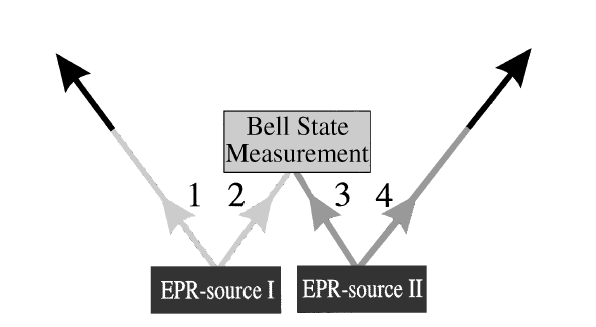
\includegraphics[width=120mm, keepaspectratio]{osszfonmeg1}
\caption[Összefonódás megosztás elvi rajza]{Összefonódás megosztás elvi rajza: Két összefonódott pár forrás (EPR source I és II) összefonódott fotonpárokat bocsájt ki(1-2 és 3-4). Mindegyik párból 1-1 fotonnal (2 és 3) végrehajtunk egy közös Bell mérést, aminek hatására a maradék két foton(1 és 4) is összefonódott állapotba kerül.}
\end{figure}
Megjegyzendő még érdekességként, hogy Peres elméletének megfelelően\cite{peres2000delayed} az összefonódás megosztás akkor is végbemehet, ha a (jelen esetben Alíznál) Bell mérést csak azután hajtjuk végre, hogy Bobnál már megmértük a másik két(jelen példánál A és D) állapotokat. Ezt igazolja például egy 2012-es kísérlet is\cite{ma2012experimental}.
\\
\begin{figure}[H]
\centering
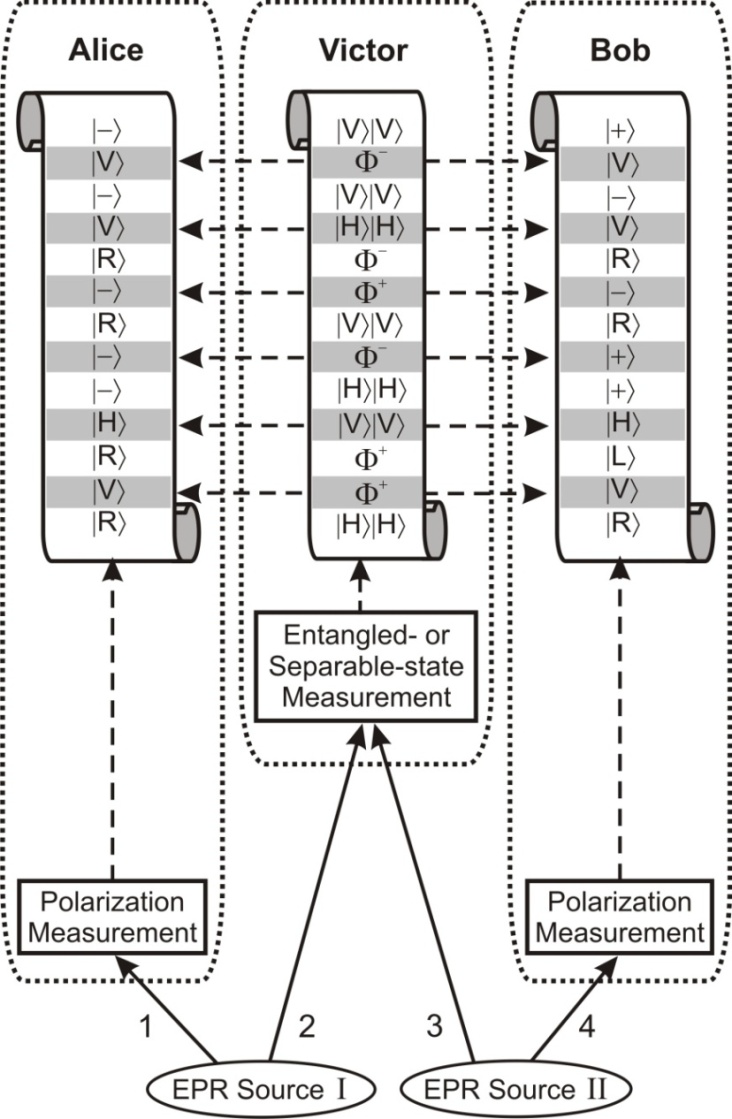
\includegraphics[width=120mm,keepaspectratio]{delayedchoice}
\caption[Késleltetett összefonódás megosztás kísérlet]{Elvi kísérleti összeállítás delayed choice(késleltetett döntéses) összefonódás megosztás vizsgálatára. Az előzőekhez hasonlóan itt is két összefonódott pár forrás szolgáltatja a fotonpárokat, viszont a korábbiakkal ellentétben itt először az 1-es és 4-es foton állapotait nézzük meg, utána véletlenszerűen döntünk, hogy Bell mérést, vagy valamilyen szétválasztható állapot szerinti mérést végzünk el. Ezek után Alice és Bob rendezni és vizsgálni tudja a már meglévő mérési adatait Victor döntése ismeretében. Azt kapjuk, hogy Alice és Bob fotonjai vagy összefonódott vagy szétválasztható állapotokként viselkednek, Victor mérési eredményeinek megfelelően.}
\end{figure}

\subsection{Összefonódás megosztások összefűzése}

Tekintve, hogy milyen fontos szerepe van az összefonódásnak a kvantumkommunikáció területén, az összefonódás megosztás is egy fontos eljárása, építőeleme számos kvantumkommunikációs protokollnak. Ezek közül talán az egyik legfontosabb ilyen felhasználási terület a kvantum ismétlők. A kvantumkommunikációs csatornák a valóságban nem tekinthetőek tökéletesnek, hasonlóan a klasszikus összeköttetésekhez, itt is számolni kell például csillapítással(hosszabb távon komoly probléma például a fotonok elnyelődése, detektálásuk nehézsége), a környezet hatásaival, mint például dekoherencia,zaj. Ebből adódóan nem élhetünk azzal a feltételezéssel, hogy hosszabb kapcsolatoknál az elküldött információnk a fogadó oldalra eredet formájában jut el. A kvantum csatorna átvitelére jellemző exponenciális csökkenés pedig gyakorlatilag ellehetetleníti a hosszabb távokon át történő információátvitelt. Erre lehetne az egyik megoldás, a klasszikus kommunikációhoz hasonlóan, ha megfelelően nem túl nagy távolságonként ismételnénk, eredeti állapotában mindig újra küldenénk tisztábban. A klasszikus kommunikációban ez könnyedén megoldható, azonban a kvantumos másolási tétel (No Cloning Theory) miatt nem lehet azt a megoldást teljes egészében lemásolni.Vegyük észre viszont, hogy a kvantum teleportációs protokoll segítségével tetszőleges állapotot tudunk elvinni egyik helyről a másikra, feltéve hogy a cél és a forrás rendelkezik egy összefonódott párral amin már előzőleg megosztottak.A problémát ily módon vissza tudjuk vezetni összefonódott párok szétosztására(mert klasszikus információt már tudunk nagy távolságokra is szállítani).Összefonódott párokat különben sem csak a teleportációs protokoll használ működése során, két hely közötti összefonódásra tekinthetünk egy általában is értékes erőforrásként. Itt lehet segítségünkre az összefonódás megosztás jelentősége.  
 
Természetesen az összefonódott párokat akarunk szétosztani ugyanúgy fennállnak az előzőleg említett problémák a csatornával, viszont tekintsük a következő esetet\cite{goebel2008multistage}: Ha az összefonódott párok közül az egyiket előzőleg összefonódás megosztásával hozzuk létre, könnyen elképzelhető, egy szabadon bővíthet séma, ahol a nagy átviteli távolságot, többszöri összefonódás megosztásával több kisebb szakaszra lehet bontani.
Vizsgáljuk meg azt az esetet amikor ezt a hosszabb távot két részre osztjuk fel. Ilyenkor kétszer kell összefonódást megosztani, három összefonódás forrásunk van, és két Bell mérést hajtunk végre a párjaink. Ha a párjaink kezdetben 1-2 3-4 és 5-6, akkor a Bell méréseket hajtunk végre 2-3-on és 4-5-ön. Ennek eredményeként 1 és 6 kerül összefonódott állapotba.
\\

\begin{figure}[h!]
\centering
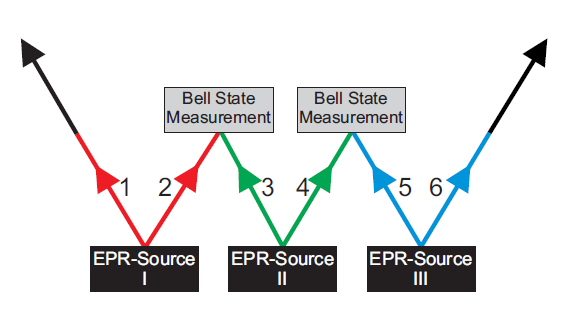
\includegraphics[width=120mm,keepaspectratio]{swapconcat}
\caption[Összefonódás megosztások összefűzése]{Többlépcsős összefonódás megosztás elvi felépítése:\\
A források által(EPR-Source I-II-III) kiadott kezdeti összefonódott párok: 1-2, 3-4, 5-6. 2 és 3-on majd 4 és 5-ön elvégezzük a Bell mérést. A két Bell mérés hatására végül 1 és 6 kerül összefonódott állapotba.}
\end{figure}

Felírva a rendszer állapotát:
\begin{center}
$ \ket{\Psi}_{123456}= \ket{\Psi^-}_{12} \otimes \ket{\Psi^-}_{34} \otimes \ket{\Psi^-}_{56} $
\end{center}
Ez átírható a következő alakra:
\begin{center}
$ \ket{\Psi}_{123456} = \frac{1}{2} \Big[ \ket{\Psi^+}_{14}\ket{\Psi^+}_{23}-\ket{\Psi^-}_{14}\ket{\Psi^-}_{23}-\ket{\Phi^+}_{14}\ket{\Phi^+}_{23} + \ket{\Phi^-}_{14}\ket{\Phi^-}_{23} \Big] \otimes \ket{\Psi^-}_{56} $
\end{center}
A korábbi két fotonpáros esethez hasonlóan itt is megfigyelhető, hogy az 1-es és 4-es fotonok a Bell mérés után összefonódott állapotban lesznek a mérés eredményétől függetlenül. Az eredmény csak arról szolgáltat információt, hogy melyik összefonódott állapotban vannak,, mivel az most is egyezik 2-3 közös mért állapotával.
Ha feltesszük, hogy 2-3-as fotonpárnál $ \ket{\Phi^-} $   állapotot mértünk, a fennmaradó 4 fotonos rendszer a továbbiakban a következő formában írható fel:
\begin{center}
$ \ket{\Psi}_{1456} = \frac{1}{2}\Big[ \ket{\Psi^+}_{16}\ket{\Phi^-}_{45}+\ket{\Psi^-}_{16}\ket{\Phi^+}_{45} - \ket{\Phi^+}_{16}\ket{\Psi^-}_{45} - \ket{\Phi^-}_{16}\ket{\Psi^+}_{45} \Big] $
\end{center}
Hasonlóan az előzőekhez, elvégezzük a Bell mérést 4-5-ön, aminek hatására 1 és 6 összefonódott állapotba kerül. A mérési eredménynek megfelelően például, ha a Bell mérésnél $\ket{\Phi^-} $ állapotot mérünk, akkor 1-6-nak az állapota: $ \ket{\Psi^+} . $ \\
A folyamat a fentiekből kiindulva általánosítható több tetszőleges számú összefonódott párral, tetszőleges számú Bell-méréssel, amivel az áthidalni kívánt távolság is tetszőleges számú szakaszra bontható fel.\\
A itt ábrázolt módszer is még idealizált csatornákkal dolgozik, magában nem oldja az előzőleg említett problémákat, mégis egy fontos építőeleme a későbbi ismétlő létrehozására irányuló modelleknek.
%%%
\subsection{A kvantum ismétlő}
%%%
A kvantum ismétlő megvalósítására törekvő modellek túlnyomó része három fő építőelemből áll, és jellemzően e három építőelem más és más megvalósításában tér el egymástól.Egy jellemző általános megvalósítás az alábbi:
A nagy távolságon jelentkező romlás elkerülése végett, ezt a távolságot felosztjuk több kisebbre, amik között a fentebb részletezett módon összefonódás megosztással teremtünk kapcsolatot. A felosztott kis távolságok között állomásokat alakítunk ki(ismétlőket), itt végezzük el az összefonódás megosztáshoz szükséges Bell méréseket. Továbbá minden szakaszhoz(minden összefonódás megosztási lépcsőhöz) létre kell hoznunk plusz összefonódott párokat amiket a folyamat során elhasználunk. Ehhez szükségünk van egy összefonódott pár forrásra, ami manapság már igen sokféle lehet[].Ez az egyik fő hasonlóság és egyben különbség is a legtöbb megvalósításban. A csatorna nem ideális átvitelével még mindig nem foglalkoztunk, pedig látható, hogy az továbbra is exponenciálisan fog romlani a csomópontok és a hossz növelésével. Ennek kiküszöbölésére használhatunk valamilyen összefonódás tisztító eljárást. Ezek jellemzően több nem teljesen tiszta összefonódott állapotból állítanak elő kevesebb, tisztább, jobban összefonódott állapotok.Tipikusan van egy tisztasági határérték a felhasznált “koszos” összefonódott állapotokra ami fölött alkalmazhatóak, emiatt akár ezek paraméterei támaszthatnak határokat a csatornaszakaszok hossza felé. Segítségükkel az átviteli sebesség kárára ugyan, de az átviteli folyamatok közé megfelelően beiktatva, kompenzálhatóak a csatornából származó veszteségek. \\
\underline{Példa egy tisztító protokollra}\\
Egy lehetséges ilyen tisztító protokoll például a Bennett által javasolt[8] aminek folyamán helyben végzett transzformációk segítségével több nem teljesen “tiszta” összefonódott párból kevesebb jobban összefonódott állapot hozható létre. (Megemlítendő, hogy eredetileg elektronspinekre írták le, de természetesen megvalósítható más hordozók esetén is.) Legyen M egy “kevert”(nem tiszta) állapot amiből tisztább, jobban összefonódott állapotokat szeretnénk létrehozni. (Ilyen lehet például egy zajos csatornán megosztott $ \ket{\Psi^-} $  pár.) Ilyenkor M tisztaságát az eredeti teljesen összefonódott állapothoz képest 





\chapter{Szimuláció}

A szimuláció elsődleges célja egy általános kvantum ismétlő protokoll működésének vizsgálata. Ennek megfelően a különböző fizikai megvalósítások pontos szimulációjától ezek sokszínűsége miatt a továbbiakban eltekintettem, helyette egy általánosított modellen vizsgáltam az egyes paraméterek hatását. A modell elemei a bevezetőnek megfelelően ismétlő állomások és csatornák. Az állomások rendelkeznek kvantum memóriákkal, képesek mérések, és helyi műveletek elvégzésére a memóriájukban tárolt qubitjeiken, valamint egy speciális állomásfajtának tekinthetjük az összefonódott pár forrásokat is. A csatornák az állomásokat összekötő kommunikációs összeköttetések, amelyeken keresztül a qubitjeinket az állomásoknak szétküldjük. Továbbá feltételezzük, hogy az egyes állomások képesek egymás közt hagyományos kommunikációra is. 

\section{Választott környezet, eszközök}

A szimuláció c++ nyelven íródott(c++11-et használ),valamint az Eigen \cite{eigen}  lináris algebra könyvtárt használja. Az elkészítésnél cél volt sokféle szimulációs elrendezés támogatása, emiatt használata a legtöbb esetben egy c++ könyvtáréhoz hasonló. A legegyszerűbb esetben egy előre megírt függvény egyszeri meghívásával akár egy teljes szimuláció is futtatható, viszont a rendelkezésre álló eszközökkel lehetőség van teljesen egyedi szimulációs elrendezés készítésére is. Az egyes elemek 4 fő csoportba sorolhatók, melynek megfelelően az egyes funkciók 4 header fájlba kerültek szétosztásra. Ezek: a kvantumos elemek reprezentációit tartalmazó, az ismétlő protokoll elemeit tartalmazó, a szimuláció vezérléséért felelős, valamint az előre megírt teszteseteket  tartalmazó fájlok.
\section{A szimuláió vezérlése}
A szimuláció vezérlése egy végrehajtási lista alapján történik, melynek kezelését a \texttt{SimRoot} és \texttt{SimItem} osztályok végzik. A lista \texttt{SimItem} típusú elemekből áll. Ebben az osztályban találhatók infromációk az egyes elemek egymáshoz képesti viszonyáról a sorban, valamint a végrehajtandó lépéseket is itt tárolódnak. Egy ilyen lépést egy itt tárolt függvény (std::function) jelképez ami végrehajtáskor meghívódik. Ilyen függvény lehet például egy Bell-mérés végrehajtása, vagy egy qubit átküldése egy csatornán. Ezen felül tárolva van még a végrehajtás tervezett ideje is. A listát kezelő \texttt{SimRoot} osztály ennek alapján új elem felvételénél a megfelelő helyre tudja rakni a tagokat ezzel egy idő szerint rendezett struktúrát hozva létre. A végrehajtásnál így már mindig csak a soron következő  elemmel kell foglalkozni.  Az objektumba felelős még a sor megfelelő ürítéséért is törlésnél, valamint itt található a szimuláció aktuális órája is.
E két osztály a \texttt{Simulation.h} fájlnak része.

\section{A kvantumos elemek reprezentációja}

A szimuláció során elemi kvantumos egységnek nem a kvantum bitet, hanem mivel minden esetben egy vagy több párral kell dolgozni a kvantum bitpárt választottam. Ennek leírására \texttt{qrep.h} fájlban található \texttt{QPair} osztály szolgál. Párt választani alapelemnek abból a szempontból is nagy könnyebség, hogy a két részecske közti lehetséges összefonódást a bitek együttes állapota már tartalmazza, ezért annak külön kezelésével nem kell foglalkozni. Az együttes állapot leírására ennek megfelelően egy 4 dimenziós komplex vektor szolgál(a 2 bit egy 4 dimenziós állapotteret feszít ki).  Ide sorolató továbbá még az egybites kvantumos memóriát reprezentáló \texttt{QMem} osztály. Az egy qubitre való hivatkozáshoz itt tárolva van a pár címe, aminek a tárolt qubit a része, valamint egy index aminek segítségével a összetett páros állapotból ki tudjuk nyerni a számunkra érdekes qubitet. Az objektum tárolni tudja még ezen kívül egy adott qubit beérkezési idejét is, amiből így később számítható a bit teljes memóriában töltött ideje. A két osztál az említetteken túl egyéb szimulációt segítő segédváltozókat tartalmaz még.

\section{Az ismétlő protokoll elemei }

Az ismétlő protokoll működéséhez szükséges elemeket az \texttt{elements.h} fájl tartalmazza. Itt vannak meghatározva a csomópontok, csatornák, valamint az általuk használt eszközök, eljárások. Ezek közül egyik másik erősen épít egymásra. Az itt található fontosabb dolgok ezt is figyelembe véve:\\
\underline{\texttt{Pair2Measure}} osztály ami párokon elvégzendő mérések megvalósítására szolgál. Jelen esetben csak a Bell-mérés megvalósítására szolgál, viszont megfelelő paraméterekkel más mérések is elvégezhetőek. Mérést tud végezni 2 páron.  Ehhez mivel a párok közötti összefonódással számolni is számolni kell létrehozza az így kialakuló minde a két párra kibővített teret és a továbbiakban azon dolgozik. Magát a mérést a bevezetőben leírtak szerint el lehet végezni. Továbbá tartalmaz állítható kisegítő mátrixokat is, amivel például egyszerűbb bázisváltás is végezhető, megfelelő beállításukkal a mérési folyamat tovább egyszerűsíthető. A beépített Bell-mérés(\texttt{.bmeasure()}) ezeket használja, emiatt a beállításuk fontos, viszont ez egyszerűen megtehető egy másik beépített függvénnyel(\texttt{.SetBellMeasure()}).\\
\underline{\texttt{EPR}} osztály, ami összefonódott párok előállításáért felel. Benne állítható a létrehozni kívánt pár(ez bármilyen lehet) állapota, amit itt is egy 4 dimenziós komplex vektor ír le, valamint a kiadott pár ehhez képesti tisztasága, amivel egy ismeretlen zaj hatását lehet imitálni. Beállítható még a pár generálások közt eltelt idő, ami később a szimulációban kerül felhasználásra.\\
\underline{\texttt{Channel}} osztály az egyes csomopontokat összekötő kvantumos kommunikációs csatornák leírására. Az egyes csatornákat a hosszukkal, valamint csillapításukkal, amit itt egy ``csillapítási hosszal'' jellemzünk. A csatorna által okozott zavar/veszteség egy bit egyszeri átküldésénél a legtöbb esetben átviteli valószínűségként nyilvánul meg. Ennek értéke az előző jellemzőkkel leírva:\\
\begin{center}
$ p=e^{-\frac{L}{L_{cs}}}$, ahol $L$ a teljes hossz $L_{cs}$  pedig a ``csillapítási hossz''.\\
\end{center}
Ezeken felül az osztály tartalmaz még a szimulációt segítő egyéb változókat(pl.: melyik két csomópontot köti össze), valamint egy a szimulációs sorban végrehajtandó lépést is. A \texttt{SendThrough} függvény írja le azt, hogy mi történik a qubittel a csatornán való áthaladás során. A csatorna jellemzőinek megfelelően módosítja a qubitet tartalmazó pár állapotat, valamint lépteti tovább a szimulációt azáltal, hogy a végrehajtási sorba beütemezi a következő lépést.\\
\underline{\texttt{Node}} osztály felelős a használt csomópontok leírásáért. El vannak benne tárolva a csomópont működéséhez szükséges információk:  a csomópont helye a felépített kísérleti rendszerben(a többi csomóponthoz képest), a működése során felhasznált eszközök(Bell-mérés, pár létrehozás, pár tisztítás). Ezeken felül minden ilyen csomópont rendelkezik valamennyi memóriával is(\texttt{QMem} tömb) amiken keresztül működése során az egyes qubiteket manipuláln tudja. Az összefonódott párokat létrehozó egységeknél állítható plusz változó még az egyszerre létrehozandó párok száma, valamint a mérést végző egységek esetében a tisztító protokoll által elérendő tisztaság. Az osztályban van még definiálva a végrehajtási sorban fellelhetó szimulációs lépések nagy része is.

\section{Szimuláció működése}

A szimuláció és az alkalmazott modell működésének bemutatásához tekintsük a következő egyszerű esetet. A vizsgált rendszerben két végpont között egy csomópont, valamint két összefonódott pár forrás segítségével szeretnénk összefonódott állapotokat megosztani. Így összesen 5 egységünk és 4 csatornánk van:3 hagyományos csomópont és 2 párt generáló, valamint az őket összekötő csatornák. A továbbiakban egy pár útját vizsgáljuk ahogy halad és változik a rendszerben. Ehhez kiindulásak feltételezzük, hogy már vannak más párok is a rendszerben, viszont a vizsgált párunk számára is van még szabad memória.
\\
\begin{figure}
\centering
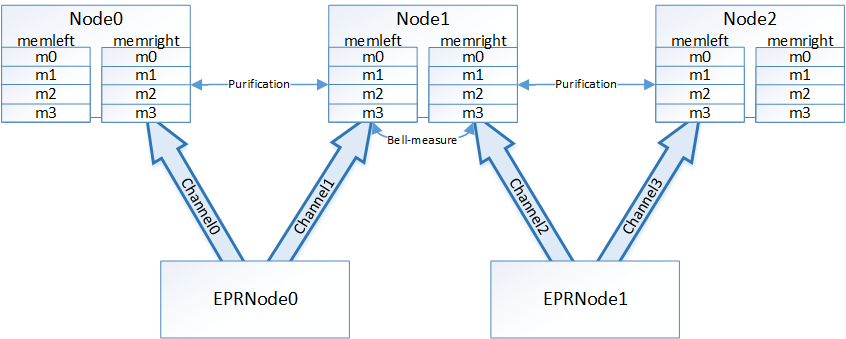
\includegraphics[width=\textwidth,keepaspectratio]{pelda}
\caption[Példa modell egy kisebb hálózatra]{Példa modell egy kisebb hálózatra\\
A vizsgált párt generálja EPRNode0. Ennek megfelelően a hozzá kapcsolódó lépések egy lehetséges sora: \\
1.EPRNode0->GenEPR : A párt létrehozza a forrás.\\
2.Channel0->SendThrough és Channel1->SendThrough: Csatornákon való átküldés\\
3.Node0->ReceiveFromCh és Node1->ReceiveFromCh: Pár qubitjeinek fogadása memóriába\\
4.Node0->ReceiveFromChSuccess és Node1->ReceiveFromChSuccess: Megbizonyosodik arról, hogy mindkét oldal fogadni tudta a pár bitjeit\\
5.Node0->Updateformeasure és Node1->Updateformeasure: Tartalmazó állomások frisstése. Mivel Node0 az egész rendszer egyik végpontja, ezért vele nem lesz több lépés, kívülről vizsgálható, hogy elkészült-e már benne a kívánt összefonódott pár.\\
6/a.Node1-> Bellmeasure: Bell mérés, ha a kétoldali memóriák állapota megfelelő\\
7/a.CorrectAfterMeasure: A pár állapotának javítása a mérési eredménynek megfelelően.\\
8/a.Node0->Updateformeasure és Node2->Updateformeasure: Az új párt tartalmazó két állomás frissítése.\\
6/b.Node1->purification:A memóriák megfelelő állapota esetén az állomáshoz tartozó tisztító protokoll elvégzése.\\
7/b.Node1->Updateformeasure: Állomás frissítése tisztítás után.
}
\end{figure}
\\
A vizsgált párt az egyik párokat generáló csomópont hozza létre a \texttt{GenEPR} lépés segítségével, ami végrehajtása során a pár létrehozásán túl késleltetve ütemezi a következő generálást. Ezen felül ütemezi a hozzá tartozó két csatornán a qubitek átküldésére szolgáló, egyes összekötő csatornák által tárolt \texttt{SendThrough} lépést, a pár megfelelő indexeivel meghívva. Amennyiben a bit átjut a csatornán, a csatorna típusának és hosszának megfelelő késleltetéssel ütemezve lesz a következő lépés ami az egyes csatornák végpontjaihoz tartozó hagyományos csomópontokon végrehajtott \texttt{ReceiveFromCh}. Itt kizárólag azt vizsgáljuk, hogy az éppen beérkező qubit számára van-e hely az egység memóriájában. Amennyiben nincs, a párt megfelelően törli, ha van, akkor pedig berakja az üres memóriába, és ütemezi a következő teendőt, valamint a csomópont struktúrában elfoglalt helyének megfelelően állítja a memória szimulációs állapotát.  Mivel a párral csak akkor tudunk a továbbiakban dolgozni, ha mind a két bitjét sikerrel fogadtuk, ezért a két fogadó csomópontnak ezt a tényt le kell kommunikálniuk klasszikus kommunikációs csatornák segítségével. Ezt a folyamatot jelképezi a megfelelő késleltetéssel ütemezett \texttt{ReceiveFromChSuccess}. Ha mindkét bit sikeresen bekerült a hozzá tartozó memóriába, állít a memória szimulációs állapotán, valamint ütemezi a következő lépést. Ez az \texttt{Updateformeasure} ami egy a csomópontot elvégzett frissítés. Azt nézi, hogy memóriákon végrehajtható-e már a Bell-mérés, valamint hogy mely tárolt párokon szükséges tisztítóprotokollt végrehajtani.
Ennek megfelelően Bell-mérés elvégzést ütemez, vagy tisztítóprotokoll elvégzést ütemez. A Bell-mérés elvégzését a \texttt{Bellmeasure} lépéssel lehet elvégezni. Ennek során a bevezetőben leírtak alapján két páron megtörténik a Bell-mérés. Végeredményül az egyik új pár(a mért bitekből keletkezett) törlődik, míg a két távoli állomás bitjei között új pár keletkezk. A mérésnek 4 eredménye lehet, de mivel a protokoll során mi egy bizonyos állapotot szeretnénk szétosztani szükség van egy mérés utáni korrekcióra. Ehhez szükség van a mérés eredményére, valamint az új pár qubitjein kell elvégezni, ezért itt is fellép a csomópontok között szükséges klasszikus kommunikációból adódó késleltetés. Ez a \texttt{CorrectAfterMeasure} megfelelő időre történő ütemezésével szimulálható. Maga a korrekció elvégezhető a qubiteken történő helyi műveletek végrehajtásával a teleportációs protokoll \cite{bennett1993teleporting} idevágó lépéséhez hasonlóan  Pauli X és Z kapuk segítségével. Legyen a cél állapotunk $\ket{\Phi^+}$. Ekkor a mérés után lehetséges 4 Bell állapotból ez csupán az első biten végrehajtott műveletekkel a következő módon előállítható:
\begin{center}
$\ket{\Phi^+} \rightarrow \ket{\Phi^+}$ \\
$Z\ket{\Phi^-} \rightarrow \ket{\Phi^+}$ \\
$X\ket{\Psi^+} \rightarrow \ket{\Phi^+}$ \\
$ZX\ket{\Psi^-} \rightarrow \ket{\Phi^+}$ \\
\end{center}
Ez után a párt tartalmazó memóriák állapotának frissítése történik, majd a pár qubitjeit tartalmazó állomások frissítése(\texttt{Updateformeasure}). Figyeljük meg, hogy ez a frissítés már a mérés utáni párt tartalmazó állomásokat frissíti, ezáltal az ismétlő protokollban soron következő mérés elvégezhetőségét ezzel a frissítéssel már vizsgáljuk.
Ha egy állomáson elég memória foglalt már, valamint a memóriákhoz tartozó párok tisztasága a mérés előtti előírtnál kisebb, a frissítés ütemezi az állomáshoz tartozó tisztító protokoll elvégzését. Mivel ennek elvégzéséhez két állomás együttműködésére is szükség van, itt is lehet számolni az ebből származó késleltetéssel, továbbá a tisztítás folyamata alatt az érintett memóriákon más feladatot sem végezhetünk. Ezt a programban a tisztítani kívánt memóriák lefoglalásával, majd a tisztítás megfelelő késleltetéssel történő ütemezésével lehet elérni. Ennek megtörténte után az állomás újboli frissítése következik. \\
A működésról általánosan elmondható, hogy alulról fölfele építkezik. Az összes lépés eredő kiváltó ingere az összefonódott párok periodikus létrehozása, amiket a rendszer utána vagy kezel, vagy nem. Egy másik lehetséges megközelítés lehetne, hogy az állomások folyamatosan szabad erőforrásaiknak megfelelően kérnek párokat a forrásoktól, viszont így szükség lenne további klasszikus kommunikáció lebonyolítására, ezért ettől a továbbiakban eltekintettem.


\chapter{Szimulációs eredmények}

Az elkészült szimuláció működésének ellenőrzésére a legegyszerűbb módszer, az általa szolgáltatott eredmények vizsgálata. Helyes működés esetén az így kapott eredmények használhatóak továbbá az ismétlő protokoll pontosabb bemutatására is. Mivel egy általánosított modellt szimulálok, a tesztesetéknél a program felé elvárás az adott esethez várt általános jelleg produkálása. Ennek előzetes meghatározásához használhatjuk az elméleti bevezetőben már megismerteket, valamint  a szakirodalomban megtalálható egyéb szimulációkat, tanulmányokat \cite{briegel1998quantum}\cite{van2009system}\cite{bernardes2011rate}. A vizsgált esetekben, amennyiben nincsen másképp említve, a következő adatokat tekintettem alapértelmezésnek. 
Az összefonódott párok előállításáért felelős állomások 10$\mu s$-ként egyszerre 5 darab 0.7-es tisztaságú párt állítínak elő. Az egyes csatornákra jellemző ``csillapítási hossz'' 20km. A méréseket végző csomópontok mindkét beérkező csatorna felé 20 memória egységgel (összesen 40) rendelkeznek, valamint az egyes mérések előtt 0.98-as előírt tisztaságig tisztíttatják a párokat. Az alapértelmezetten használt tisztító protokoll egy a bevezetőben már ismertetetthez hasonló \cite{deutsch1996quantum}, néhány későbbiekben javasolt változtatással \cite{briegel1998quantum}. Ennek lépései a programban teljes egészében, közelítések nélkül vannak szimulálva. Az egyes tisztítások sorrendjének meghatározásához használt alapértelmezett stratégia az ún. ``greedy bottom up '', aminek pontos leírásával majd a későbbiekben foglalkozom. Az egyes mérések elvégzése egy a későbbiekben tárgyalt fa szerű struktúra szerint történik. Az állomások közötti kommunikáció, valamint a pár szétosztás sebessége az optikai kábelekben jellemző $2 \times 10^8 \ m/s$. A vizsgált esetek teljesítményét az egységnyi idő alatt sikeresen megosztott párok számával mérem.

\section{Ismétlő protokoll és az egyszerű csatorna}

Első tesztesetnek azt vizsgáltam milyen távolság fölött kezd egyáltalán előnyt nyújtani a protokoll az ismétlő nélküli csatornával szemben. Tudván, hogy a csatorna átvitele a távolsággal exponenciálisan csökken, míg az ismétlőé csak polinomiálisan \cite{briegel1998quantum} azt várom, hogy kis távolságoknál egyszerűsége miatt a csatorna mutat jobb teljesítmény, míg egy bizonyos távolság felett az ismétlő. Szimulációval 5-500 km-es távolságig vizsgáltam az egyes esetek teljesítményét. Először azt az idealizált esetet tekintve, ahol csak a párok elvesztésével kell számolni, a tisztaságukkal nem (szétosztott párok tisztasága = 1) ( \ref{fig:csat1} ábra), később a csatorna esetén a végpontokban, az ismétlőknél pedig a köztes állomásokon elvégzendő tisztítás hatását is figyelembe véve (\ref{fig:csat2} ábra).
\begin{figure}[H]
\centering
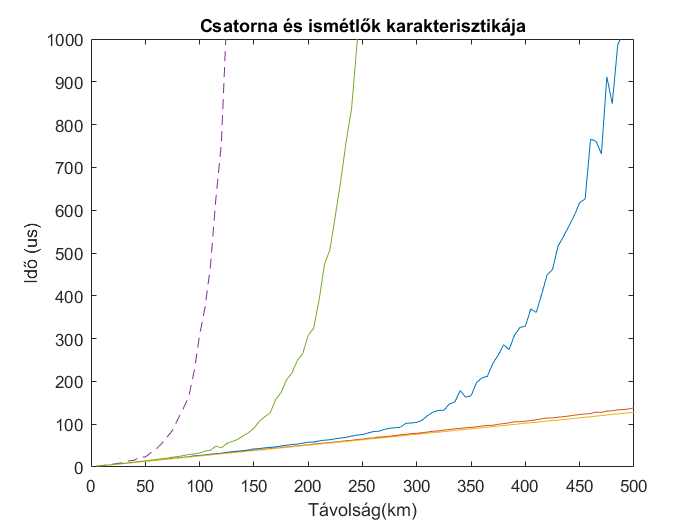
\includegraphics[width=120mm,keepaspectratio]{repvschf1}
\caption[Csatorna és ismétlők karakterisztikája 1]
{Csatorna és különböző ismétlők átvitele a távolság függvényében:\\
Az y tengelyen az egy pár megosztásához szükséges átlagos időt mérjük.\\
Lila szaggatott vonal:egyszerű csatorna.\\
zöld, kék, piros, narancs vonalak: 2, 4, 8 valamint 16, köztes létrehozó állomásból álló ismétlő rendszerek.\\
A szimuláció során kizárólag az átvitel során történő pár vesztést vizsgáltam (megosztott párok tisztasága 1-> nem kell tisztítani).\\
A csatorna és a 2 generátoros rendszer esetében a szimulációt idő előtt leállítottam a veszteségek miatt megnövekedett szükséges számítási kapacitás miatt.
}
\label{fig:csat1}
\end{figure}
\begin{figure}[H]
\centering
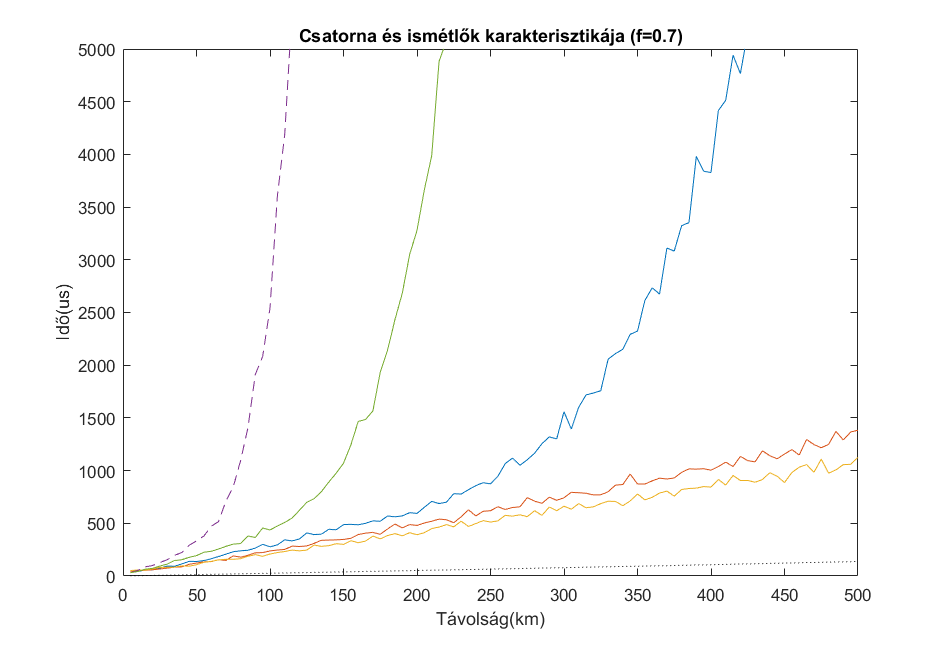
\includegraphics[width=120mm,keepaspectratio]{repvschf07}
\caption[Csatorna és ismétlők karakterisztikája 2]
{Csatorna és különböző ismétlők átvitele a távolság függvényében:\\
Az y tengelyen az egy pár megosztásához szükséges átlagos időt mérjük.\\
Lila szaggatott vonal:egyszerű csatorna.\\
Zöld, kék, piros, narancs vonalak: 2, 4, 8 valamint 16, köztes létrehozó állomásból álló ismétlő rendszerek.\\
Alsó fekete pontozott vonal: 8 köztes állomásból álló rendszer teljes tisztaság esetén.\\
A szétosztott párok ebben az esetben nem ideálisak, a tisztaságuk 0.7-es. Ennek következtében szükség van a tisztító eljárások végrehajtására. (egyszerű csatorna esetében ez a végpontokon történik.)\\
A csatorna és a 2 generátoros rendszer esetében a szimulációt itt is idő előtt leállítottam a veszteségek miatt megnövekedett szükséges számítási kapacitás miatt.
}
\label{fig:csat2}
\end{figure}
Az egyes esetek teljesítményét az egy pár megosztásához szükséges átlagos idővel mértem (200 megosztott párból számolva).
Látható a csatorna átvitelének exponenciális romlása, valamint nagyobb távolságok esetén az ismétlő elrendezések is ezt a jelleget mutatják. Ennek oka, hogy az egyes állomásokat is exponenciálisan romló csatornák kötik össze. A protokoll fő előnye, hogy egy nagy ilyen szakasz helyett használhatunk több kisebbet. A tisztaság rontásának hatása is megfigyelhető: a teljesen tiszta esethez képest ilyenkor a tisztítás miatt több párt kell felhasználni egy tiszta pár létrehozásához a végpontok között. A görbék jellege nem változott viszont az átlagos idő nőtt.\\
Az ismétlő protokollok természetesen több erőforrást használnak mint csupán egy csatorna, viszont ezzel az előzőekben nem foglalkoztam. Ennek figyelembevételre tekintettem a következő eseteket: Álljon rendelkezésre egy 8 generátoros, állomásonként 8x5 memóriaegységgel rendelkező rendszer megvalósításához szükséges erőforráshalmaz. Ebből készíthető egygenerátoros esetben egy 8-szor gyorsabb párgenerátor, valamint egyenként 8x5 pár kezelésére alkalmas végpont. Ezen logika mentén elkészíthető még 2 generátoros rendszer, 4-szer gyorsabb generátorokkal és 4x5 memóriával rendelkező állomásokkal, valamint hasonló logika alapján egy 4 és 8 generátoros rendszer is. Ezek egymáshoz képesti teljesítménye a \ref{fig:csat3} ábrán látható:
\begin{figure}[H]
\centering
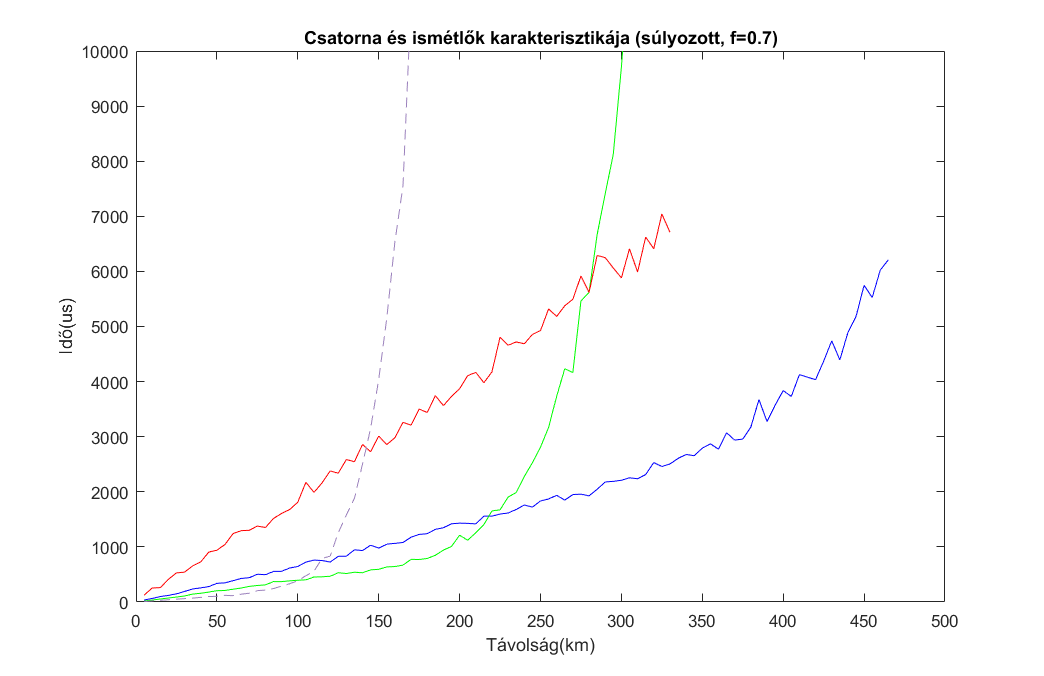
\includegraphics[width=120mm,keepaspectratio]{repvschhandicapped}
\caption[Csatorna és ismétlők karakterisztikája 2]
{Csatorna és különböző ismétlők átvitele a távolság függvényében:\\
Az y tengelyen az egy pár megosztásához szükséges átlagos időt mérjük.\\
Lila szaggatott vonal:egyszerű csatorna.\\
Zöld, kék, piros, vonalak: 2, 4, 8 köztes létrehozó állomásból álló ismétlő rendszerek.\\
A szimulációhoz szükséges idő növekedése miatt, egyes szimulációkat a páronkénti 5000 $\mu s$-os határ elérésénél leállítottam.\\
Az eredményekből látszik, hogy adott erőforrásmennyiség esetén távolságtól függően változik a leggazdaságosabb elrendezés.
}
\label{fig:csat3}
\end{figure}
Előzetes várakozásoknak megfelelően kis távolságoknál egyszerűsége miatt a csatorna teljesít jobban, egészen addig amíg az exponenciális jellegéből származó  veszteségek egy kritikus értéket meg nem haladnak. Innentől kezdve először a 2 majd 4 szegmenses ismétlő bizonyul jobbnak. A 8 szegmenses rendszerről a korábbi eredmények jellegének ismeretében feltételezhető, hogy 500-600 km-es távolság esetén már a legjobb alternatívát nyújtja, mivel 500km-hez közelítve a 4 szegmenses elrendezés is exponenciálisan kezd romlani, viszont ezek az értékek már nem tartoznak bele a szimulált tartományba. Ettől eltekintve is látszik a protokoll előnye nagyobb távolságok esetén, ami egy másik komoly optimalizálási feladatot is felvet. Korlátozott mennyiségű erőforrás esetén az adott paraméterekhez tartozó optimális méretű rendszer és az ehhez szükséges erőforrásfelosztás meghatározását.

\section{Mérési sorrend}

A protokoll működése során fontos szerepe van az egyes mérések elvégzési sorrendjének is. A következőkben két különböző stratégiát vizsgálok. Az egyik stratégia a többi vizsgálatnál általam alapértelmezettnek használt, ahol a mérések sorrendjét egy faszerű struktúra határozza meg. Itt a hálózat tipikusan $2^n+1$ elemből áll (bár a végpontoknak csak az egyik felét használjuk). Két azonos szinten lévő csomópont között a kapcsolatot mindig a közöttük félúton lévő állomáson elvégzett mérés hozza létre. Ennek egy egyszerű hálózatra történő alkalmazását mutatja a \ref{fig:sorrend1} ábra.
\begin{figure}[H]
\centering
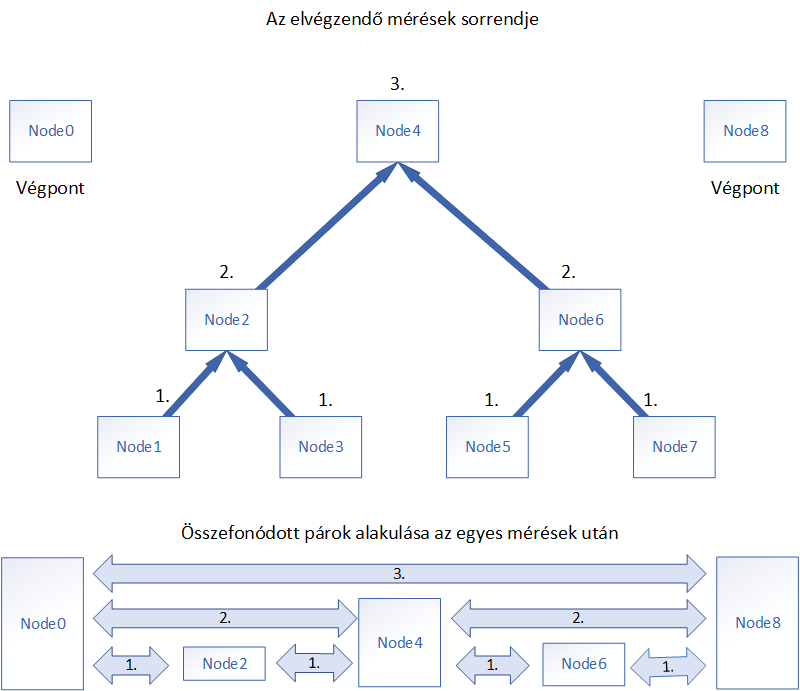
\includegraphics[width=\textwidth,keepaspectratio]{pow2tree}
\caption[Fa alapján történő mérési stratégia]{Az egyes számok a mérések elvégzési sorrendjét jelölik (feltételezzük, hogy minden állomáson rendelkezésre állnak az ehhez szükséges generátorok által küldött párok). A nyilak a sorban következő elvégzendő mérést jelölik, valamint az alsó ábrán az állomások közötti összefonódásokat.}
\label{fig:sorrend1}
\end{figure}
Az elrendezésből látszik, hogy ez a stratégia akkor a leghatékonyabb, ha $2^n-1$ közbenső állomás van (+2 végponttal lesz így $2^n+1$ állomás összesen).\\
A másik vizsgált stratégiánál egyszerűen sorban végezzük el a méréseket. Ez a \ref{fig:sorrend2} ábrának megfelelően néz ki:
\begin{figure}[H]
\centering
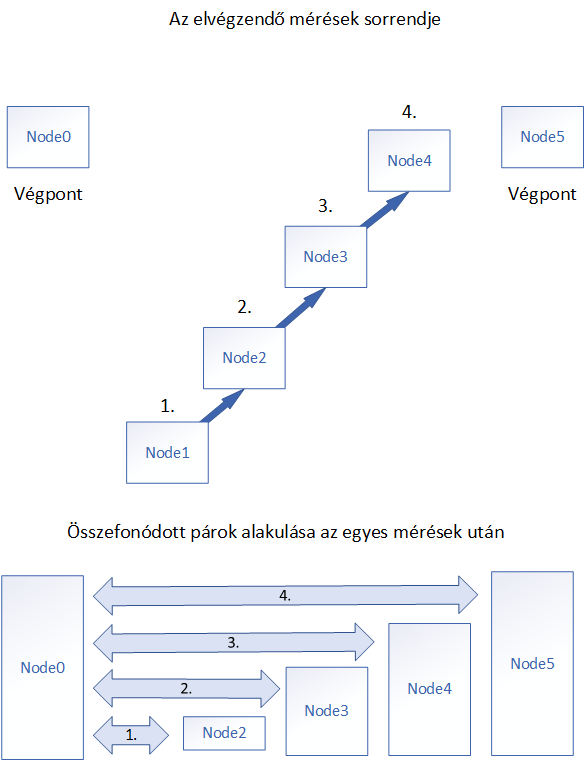
\includegraphics[width=120mm,keepaspectratio]{lintree}
\caption[Egyszerű mérési stratégia]{Az egyes számok itt is a mérések elvégzési sorrendjét jelölik (feltételezzük, hogy minden állomáson rendelkezésre állnak az ehhez szükséges generátorok által küldött párok). A nyilak a sorban következő elvégzendő mérést jelölik, valamint az alsó ábrán az állomások közötti összefonódásokat.}
\label{fig:sorrend2}
\end{figure}
Ennél a második elrendezésnél a szegmensek száma közömbös az ideális hatékonyság szempontjából. A következő szimulációknál 400 km-es távolság esetén vizsgálom az alapértelmezett paraméterek mellett a fentebb bemutatott stratégiákat (\ref{fig:sorrend3} ábra).
\begin{figure}[H]
\centering
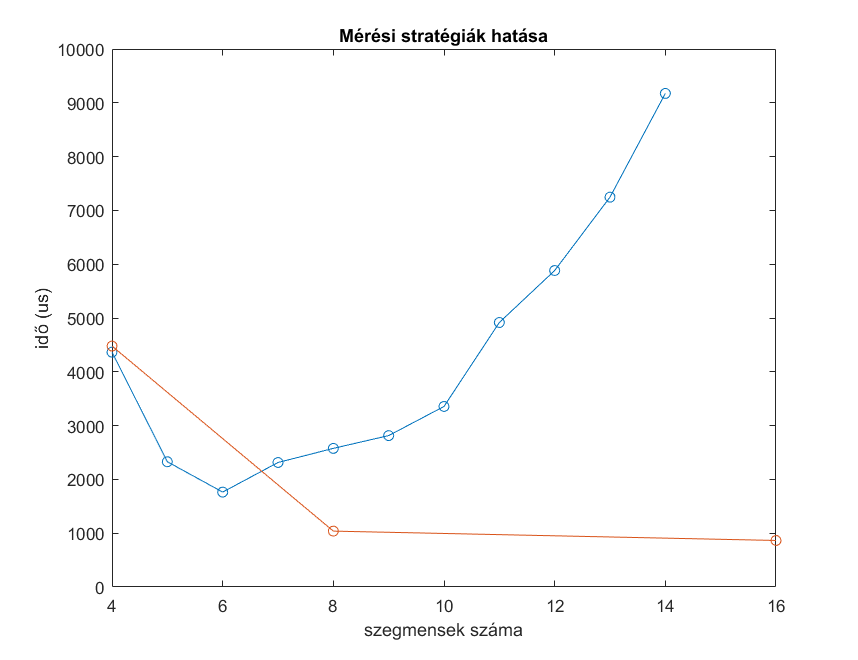
\includegraphics[width=120mm,keepaspectratio]{sorrend}
\caption[Mérési stratégiák]{A mérési stratégiák által nyújtott teljesítmények.\\
Kék vonal: egyszerű mérési stratégia\\
Piros vonal: Fa alapján történő mérési stratégia.
}
\label{fig:sorrend3}
\end{figure}
Az eredményekből látszik az első elrendezés előnye. Érdekes, hogy az egyszerű stratégia esetében a rendszer a szegmensek számának növelésével lassul. Ez az állomások számával egyre növekvő klasszikus kommunikációból származó késleltetéseknek tudható be.


\section{Összefonódott pár létrehozási sebesség hatása}

A protokoll egy fontos elemét képezik az összefonódott párok generálását végző állomások. A következőkben azt vizsgáltam, miként hat az átviteli sebességre a párok létrehozási sebességének változása. A szimulációhoz használt paraméterek a következők: Az állomások mindkét irányba 10 db memóriaegységgel rendelkeznek, valamint a generáló állomások egyszerre csak 1 db összefonódott párt állítanak elő. Az egyes párok 0.7-es tisztaságúak. Az egyes adatpontok a 200 pár megosztása során gyűjtött adatok átlagai. Az egyes szimulációkat 150 (\ref{fig:rate150} ábra), 200 (\ref{fig:rate200} ábra) és 250 km-es (\ref{fig:rate250} ábra) távolságokon végeztem.
\begin{figure}[H]
\centering
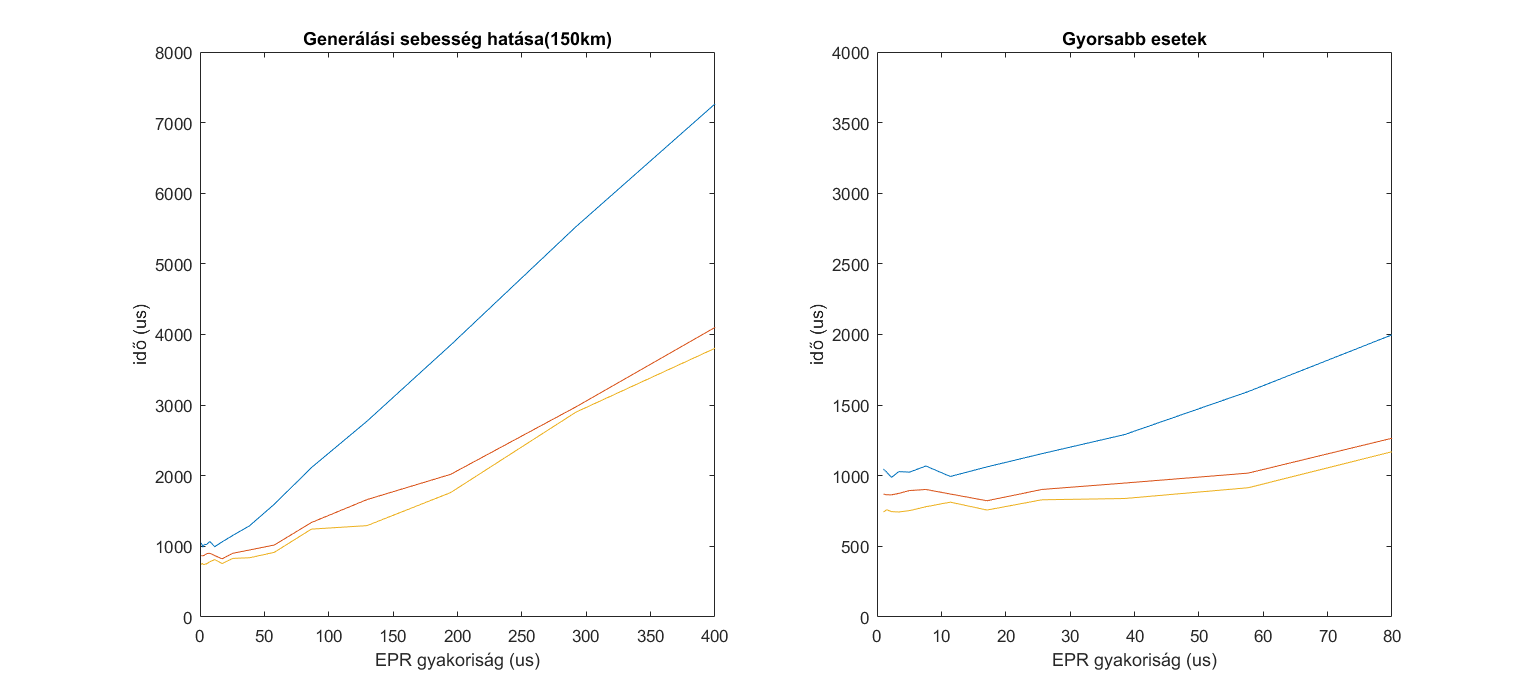
\includegraphics[width=\textwidth,keepaspectratio]{epr150}
\caption[Generálási sebesség hatása(150km)]{Generálási sebesség hatása az átviteli sebességre 150km-es szakaszon.\\
A kék,piros, sárga vonalak a 4,8,valamint 16 szegmensből álló rendszerekhez tartozó adatokat jelképezik.\\
Jobb oldalt a bal oldali grafikon kezdeti részére ráközelített kép látható.
}
\label{fig:rate150}
\end{figure}
\begin{figure}[H]
\centering
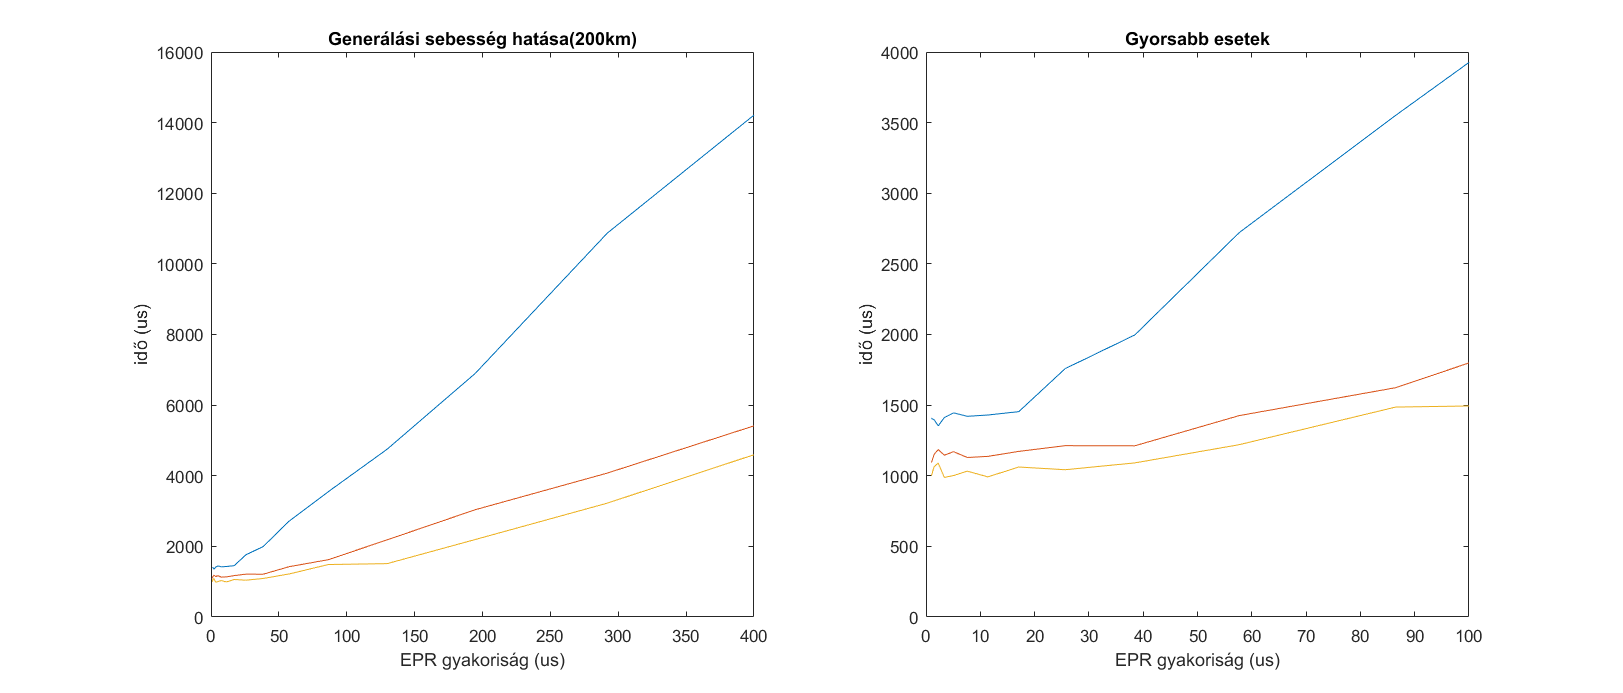
\includegraphics[width=\textwidth,keepaspectratio]{epr200}
\caption[Generálási sebesség hatása(200km)]{Generálási sebesség hatása az átviteli sebességre 200km-es szakaszon.\\
A kék,piros, sárga vonalak a 4,8,valamint 16 szegmensből álló rendszerekhez tartozó adatokat jelképezik.\\
Jobb oldalt a bal oldali grafikon kezdeti részére ráközelített kép látható.
}
\label{fig:rate200}
\end{figure}
\begin{figure}[H]
\centering
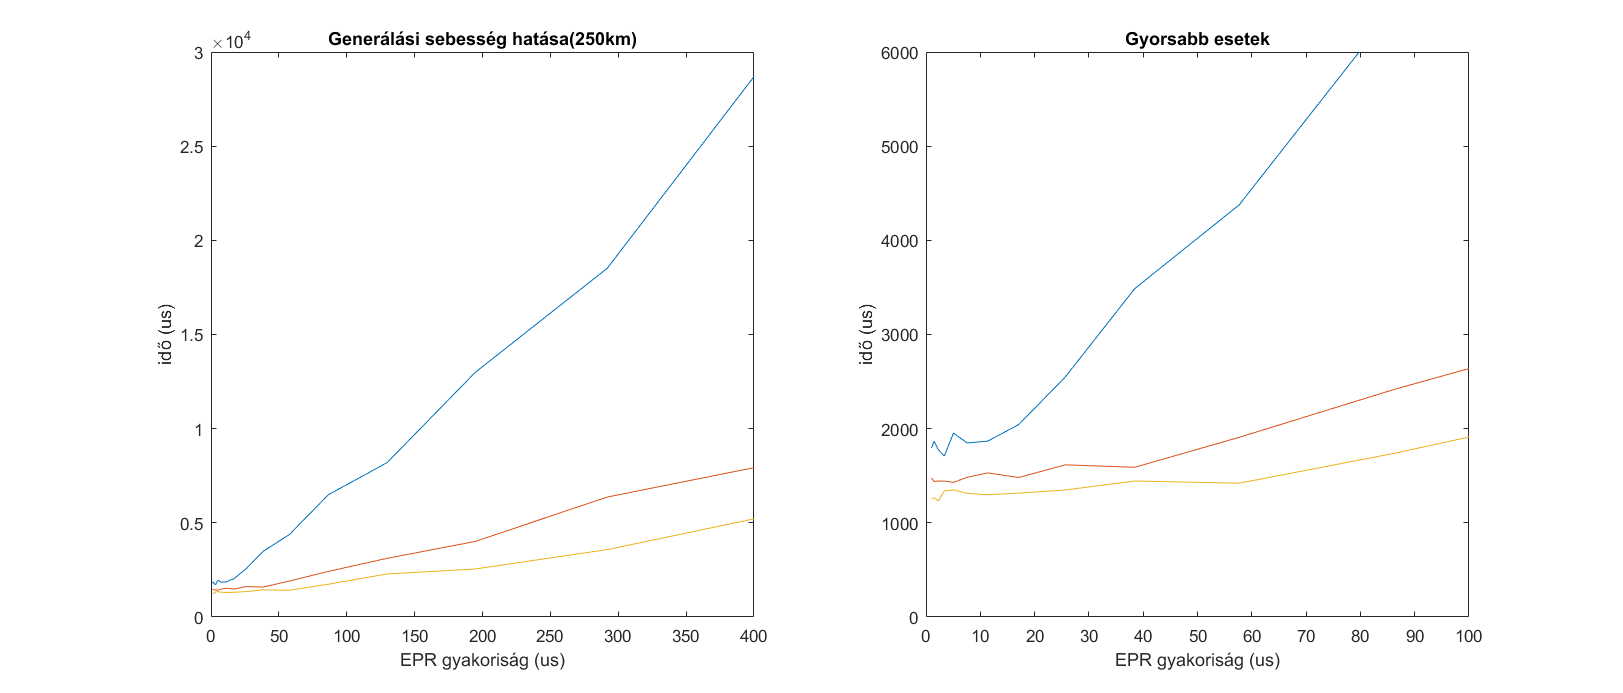
\includegraphics[width=\textwidth,keepaspectratio]{epr250}
\caption[Generálási sebesség hatása(200km)]{Generálási sebesség hatása az átviteli sebességre 200km-es szakaszon.\\
A kék,piros, sárga vonalak a 4,8,valamint 16 szegmensből álló rendszerekhez tartozó adatokat jelképezik.\\
Jobb oldalt a bal oldali grafikon kezdeti részére ráközelített kép látható.
}
\label{fig:rate250}
\end{figure}
Figyeljük meg, hogy a nagyon gyors sebességeknél (~5-10 $\mu s$/pár alatt) már nem gyorsul tovább a rendszer. Ennek oka, hogy ennél a generálási sebességnél a generáló állomások a fogadók memóriáját már szinte folyamatosan telítve tudják tartani, így a protokoll többi részének elvégzése (mérések, egymás közti kommunikáció) adja a megosztáshoz szükséges idő jelentős részét. Lassabb sebességek esetén viszont az látszik, hogy az átvitel közel egyenesen arányos a párok generálásának sebességével. Ebben az esetben a fogadó állomások már nincsenek telítődve, így a megosztáshoz szükséges idő jelentős részét a párokra való várakozás adja.


\section{A fogadott párok tisztasága}
A fogadott párok tisztaságának is hatása van a protokoll sebességére. A tisztítóeljárásokról általánosan elmondható, hogy a művelet utáni tisztaság, valamint a tisztítás sikerességének valószínűsége is függ az elhasznált párok tisztaságától. Ebből következik, hogy minél ``koszosabbak'' a fogadott párjaink, annál többre van szükség belőlük egy megfelelően tiszta állapot előállításához. Ennek hatását vizsgáltam az alábbi szimulációs esetekkel:\\
A paraméterek az alapértelmezettek, a párok tisztaságának kivételével. Az egyes eseteket 150 (\ref{fig:fid150} ábra), 200 (\ref{fig:fid200} ábra) és 250 km-es  (\ref{fig:fid250} ábra) távolságokon vizsgáltam.
\begin{figure}[H]
\centering
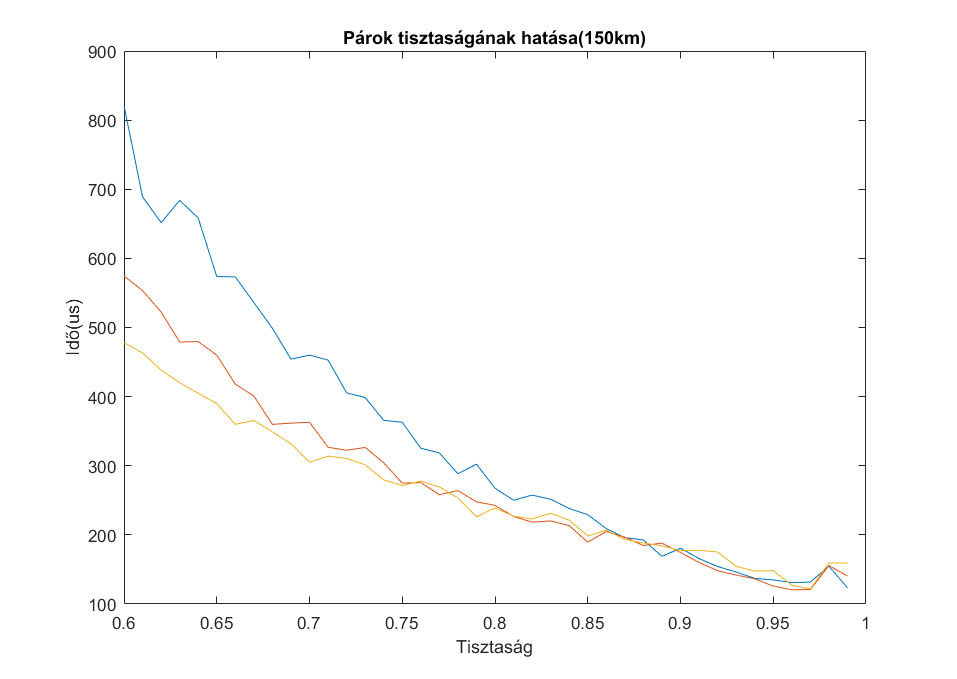
\includegraphics[width=120mm,keepaspectratio]{fidtest150}
\caption[Tisztaság hatása 150]
{Tisztaság változtatásának hatása 150 km-en.\\ 
Kék, piros, sárga vonalak: 4, 8, 16 szegmensből álló rendszerekhez tartozó adatok.\\}
\label{fig:fid150}
\end{figure}
\begin{figure}[H]
\centering
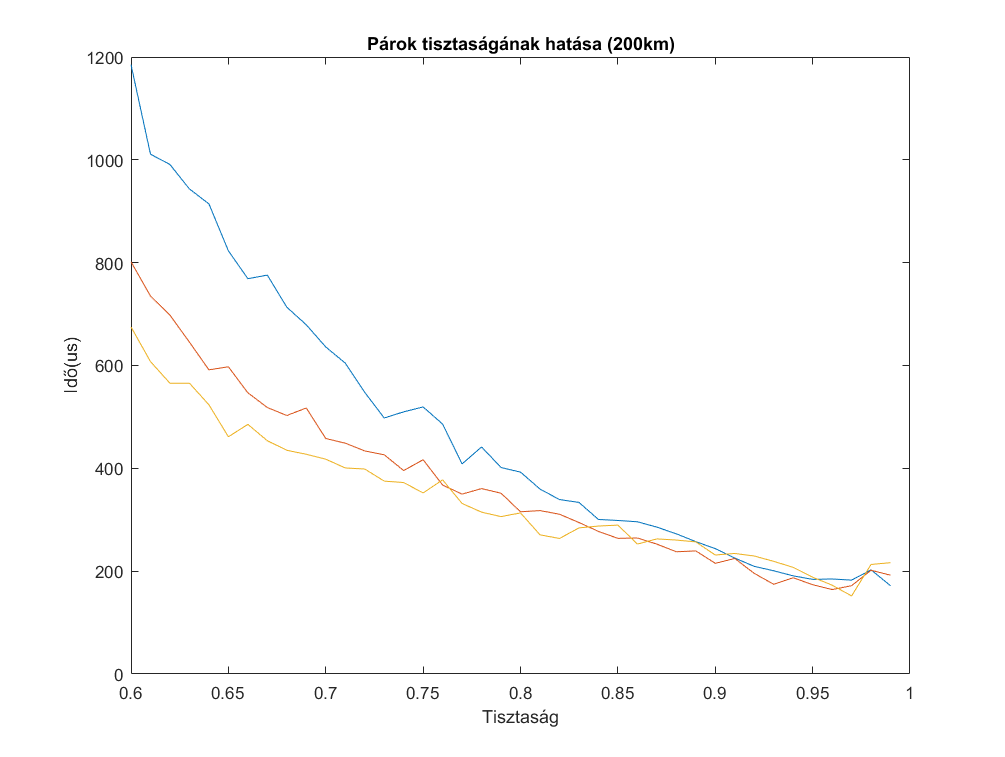
\includegraphics[width=120mm,keepaspectratio]{fidtest200}
\caption[Tisztaság hatása 200]
{Tisztaság változtatásának hatása 200 km-en.\\ 
Kék, piros, sárga vonalak: 4, 8, 16 szegmensből álló rendszerekhez tartozó adatok.\\}
\label{fig:fid200}
\end{figure}
\begin{figure}[H]
\centering
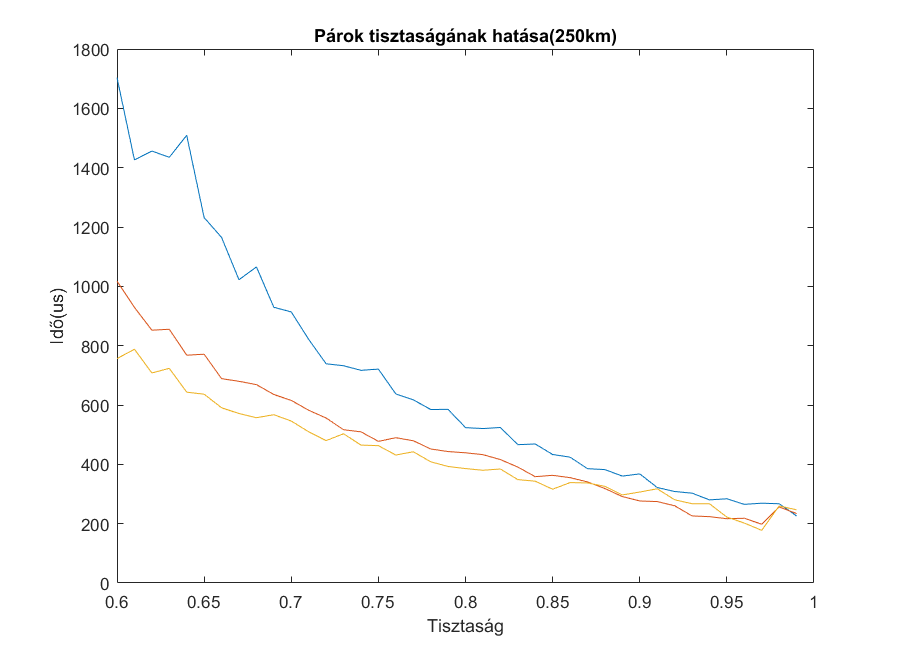
\includegraphics[width=120mm,keepaspectratio]{fidtest250}
\caption[Tisztaság hatása 250]
{Tisztaság változtatásának hatása 250 km-en.\\ 
Kék, piros, sárga vonalak: 4, 8, 16 szegmensből álló rendszerekhez tartozó adatok.\\}
\label{fig:fid250}
\end{figure}
Az eredményekből látható, hogy minél kisebb a kezdeti tisztaság, az átviteli sebesség annál erősebben csökken. Megfigyelhető továbbá, a több szegmensből álló rendszerek növekvő előnye a kisebb értékek esetén. Egy megfontolandó technikai korlát, hogy a legtöbb tisztító eljárás 0.5-ös tisztaság alatt nem működik, emiatt arra az értékre egy abszolút alsó határként is tekinthetünk.

\subsection{Tisztító stratégiák}
Az elvégzendő tisztítások sorrendje, valamint a tisztított párok párosításának módja is hatással lehet a teljesítményre. Az eddigiekben úgynevezett ``greedy bottom up'' eljárás szerint végeztem el az egyes lépéseknél a tisztítást, ami a egyszerűen annyit jelent, hogy minden egyes tisztítási lépésben először a kisebb tisztaságú párokat tisztítom egymással, valamint az összes rendelkezésre álló tisztítható párt tisztítom. Ezen annyit változtattam, hogy egy ilyen tisztítási lépés akkor ütemeződik csak, ha a szabad memóriák száma egy adott küszöb alá kerül (fel kell szabadítani, hogy fogadhatóak legyenek az új párok). A most vizsgált másik tisztítási ütemezés a ``greedy top down''. Ebben mindig a nagyobb tisztaságú párokat tisztítjuk egymással, így haladva végig a rendelkezésre álló halmazon.
Az eljárások közti különbségeket a \ref{fig:pur1} ábra szemlélteti.
\begin{figure}[H]
\centering
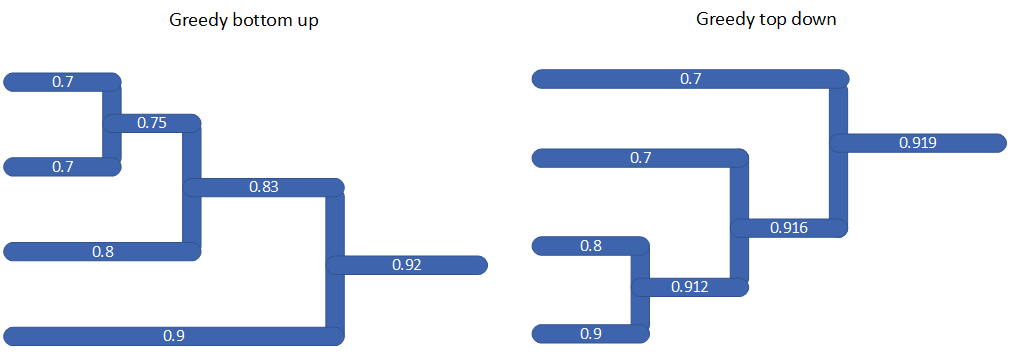
\includegraphics[width=120mm,keepaspectratio]{purifprots}
\caption[Tisztító stratégiák]
{``greedy bottom up'' és ``greedy top down'' tisztító stratégiák.\\
Az ábrán feltételezzük, hogy az egyes tisztító lépések sikeresek, valamint a keletkező új tisztaságok csak személtetésül szolgálnak, ezek pontos értéke a valóságban nagyban függ az alkalmazott tisztító eljárástól, valamint a használt párok pontos állapotától is.}
\label{fig:pur1}
\end{figure}
Az e két protokoll közti különbségeket 150km-es távon vizsgáltam.
Kapott eredményeimet a \ref{fig:pur2} ábrán foglaltam össze.
\begin{figure}[H]
\centering
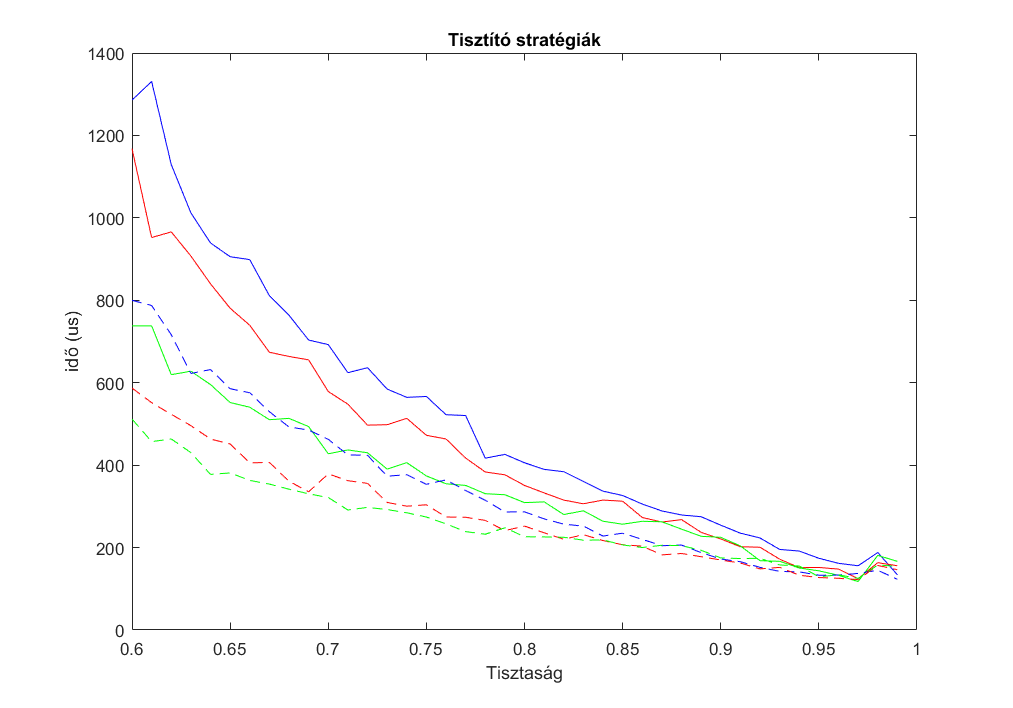
\includegraphics[width=120mm,keepaspectratio]{prottest}
\caption[Tisztító stratégiák]
{A két ismertetett stratégia teljesítményei 150 km-es távolságon \\
Kék, piros, zöld sima vonal: greedy top down 4,8 és 16 szegmenses rendszerekre. \\
Kék, piros, zöld szaggatott vonal: greedy bottom up 4,8 és 16 szegmenses rendszerekre.
}
\label{fig:pur2}
\end{figure}
A ``greedy bottom up'' előnye látszik. Ennek egyik oka az alkalmazott tisztító eljárás azon tulajdonsága, hogy a sikeresség esélye függ a felhasznált párok tisztaságától. Így a top down filozófiát követve a nagy tisztaságú párjainkat többször párosítjuk össze kisebb tisztaságúakkal, ezáltal összességében jobban kockáztatva ezen már tisztább állapotok elvesztését. A bottom up sorrendet követve viszont először mindig a koszosabb párokat használjuk el, ezáltal az értékesebb állapotokat már csak az így szerzett nagyobb tisztaságúakkal párosítjuk, ami kevésbé kockázatos.
\subsection{Tisztasági előírások}
Az előzőekben minden Bell-mérés végrehajtásához előfeltétel volt, hogy a mérésben résztvevő párok legalább 0.98-as tisztaságúak legyenek. Ezt módosítottam úgy, hogy a 0.98-as előírás csak a protokoll két végpontja között legyen érvényes, a köztes állomások az új 0.9-es határértéket használják. Ennek hatása a \ref{fig:pur3} ábrán látható. 

\begin{figure}[H]
\centering
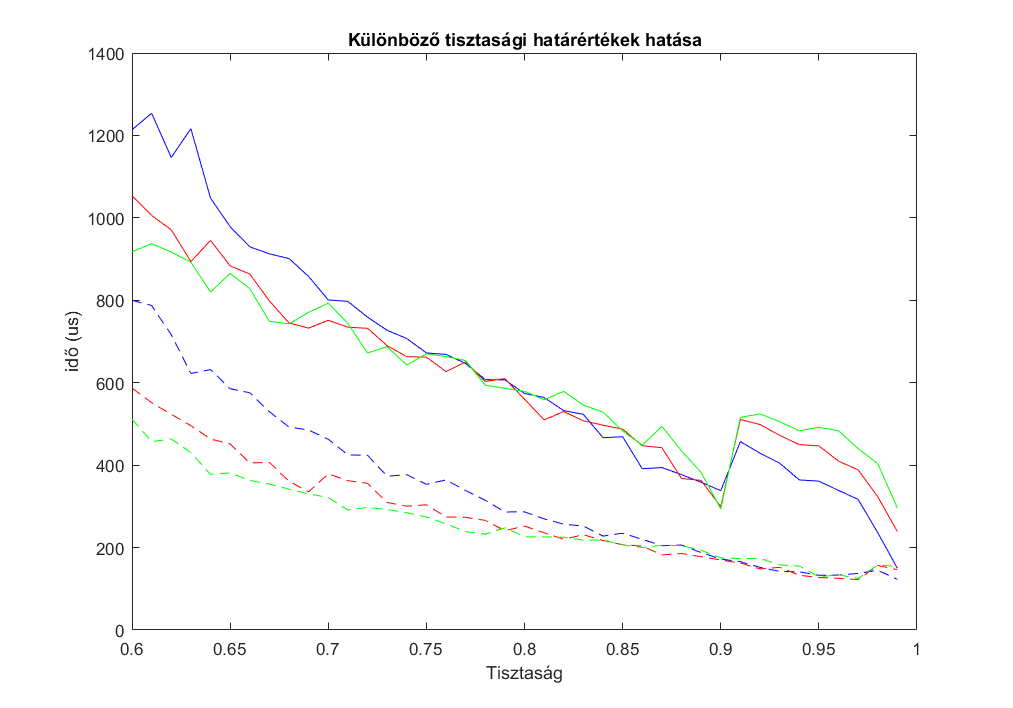
\includegraphics[width=120mm,keepaspectratio]{lowtarget}
\caption[Határérték csökkentése]
{Tisztasági előírás csökkentésének hatása150 km-es távolságon \\
Kék, piros, zöld sima vonal: csökkentett határértékkel működő rendszer 4,8 és 16 szegmens esetén. \\
Kék, piros, zöld szaggatott vonal: eredeti határértékkel működő rendszer 4,8 és 16 szegmens esetén.
}
\label{fig:pur3}
\end{figure}

Amennyiben nem tiszta állapotokon végzünk Bell-mérést, a mérés utáni állapot tisztaságáról csak azt tudhatjuk, hogy a két kezdeti állapot tisztaságának szorzatánál nem kisebb. Ebből következik, hogy a koszosabb állapotokon végzett mérés a keletkező új pár állapotát csak tovább rontja, amit utána megint tisztítani kell. A 0.9-es értéknél látható ugrás is annak köszönhető, hogy ezeken a párokon azonnal mérést végzünk, aminek hatására a következő lépésben használt párok már a kiindulásnál koszosabbak, tisztításra szorulnak. Nem megfelelő határérték esetén (pl.: < ~0.7) az is előfordulhat, hogy az alkalmazott tisztító eljárás már nem képes a Bell-mérés utáni állapot tisztítására. Szimulációs példámban látható, hogy a határérték egy kisebb változtatása is már jelentősebb romláshoz vezethet. Ugyanakkor ügyelni kell arra is, hogy ez a határérték ne legyen túl magas se, mivel a tisztító eljárások hatékonysága a teljesen tiszta állapotot közelítve romlik.

\section{Egyéb megfontolandó paraméterek}
\subsection{Protokoll indulása}
Az előzőekben kizárólag a hosszabb működés alatti átlagteljesítményt vizsgáltam, azonban meg kell említeni, hogy a rendszerek rendelkeznek egy úgymond telítődési idővel is ami indulásnál az egyes állomások kezdetben üres memóriáinak megfelelő állapotú párokkal való feltöltődésének ideje. Ennek szemléltetésére vizsgáltam a következőkben az indulástól számított első néhány sikeres megosztásig eltelt időt (\ref{fig:start} ábra).
\begin{figure}[H]
\centering
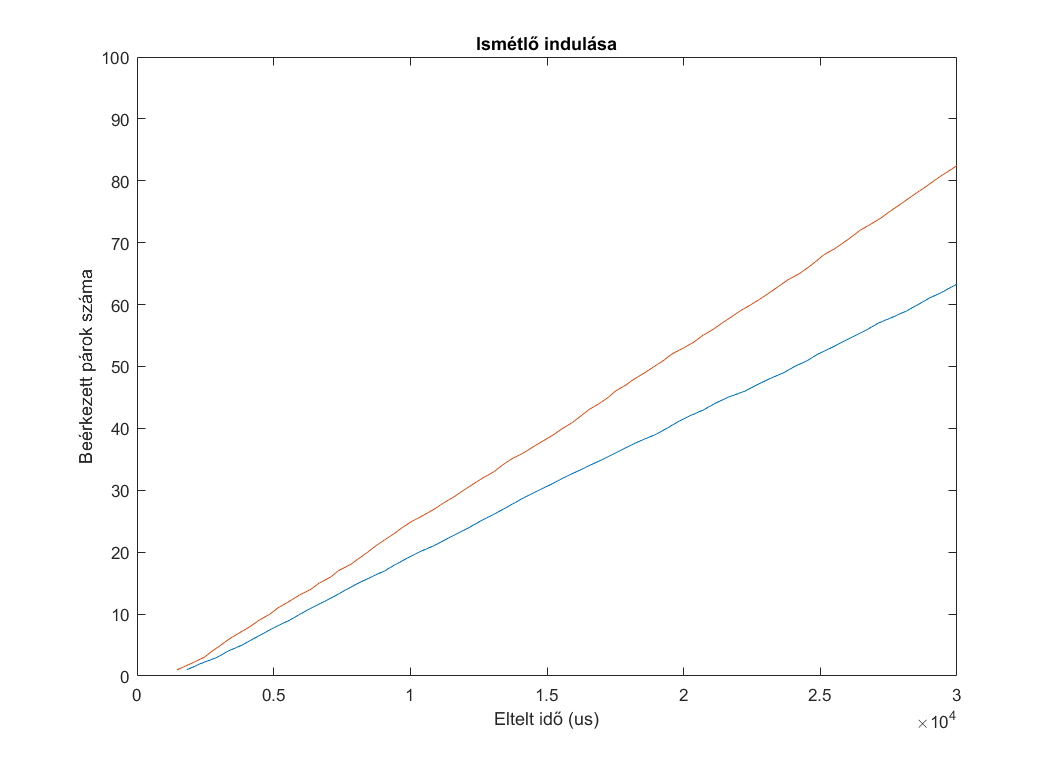
\includegraphics[width=120mm,keepaspectratio]{repstart}
\caption[Beérkezett párok indulás után]
{Beérkezett párok indulás után 150 km-es távolságnál:\\
Kék vonal: 4 szegmenses ismétlő indulása.\\
Piros vonal: 8 szegmenses  ismétlő indulása.
}
\label{fig:start}
\end{figure}
A protokoll indulásánál az első pár beérkezésére többet kell várni, mint később az egyes párok között. A rendszernek ugyanis itt teljesen üres állapotból meg kell várnia a különböző műveletek elvégzése előtt, amíg a memóriák a megfelelő állapotokkal feltelnek. (A telítődés a későbbiekben a műveletekkel párhuzamosan történik.) Ez után a telítődés után már az idővel egyenesen arányosan nő a megosztott párok száma.
\subsection{Kvantumos memóriák}
Eddig az egyes állomásokon a biteket tároló memóriákat ideálisnak tekintettük, azonban a való életben ezek korántsem azok. Határaik és tökéletlenségeik komoly limitáló tényezőt jelenthetnek. A legjobb tárolási minőségre, valamint a legnagyobb tárolási időre, a végpontokban van szükség, mivel az itt tárolt bitek állapotának fent kell maradni mialatt az összes hozzájuk tartozó mérést elvégezzük. Ennek a szükséges maximális időnek az alakulását vizsgálom az első (\ref{fig:csat2} ábra) szimulációs összehasonlítás esetében. Az így kapott memóriára vonatkozó adatok a \ref{fig:mem} ábrán láthatók.
\begin{figure}[H]
\centering
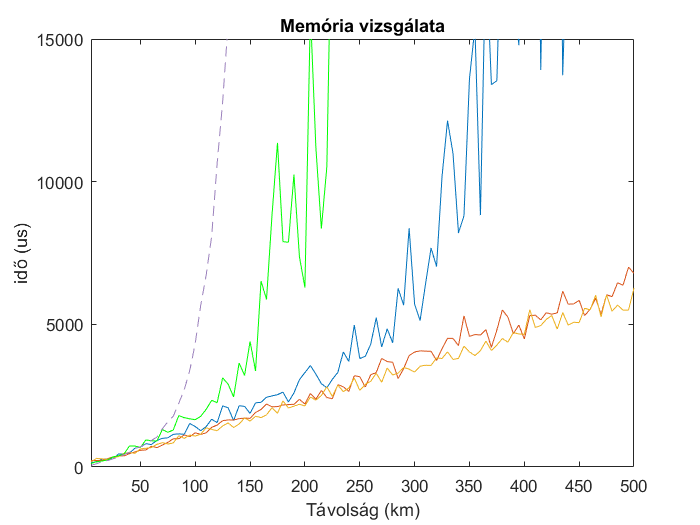
\includegraphics[width=120mm,keepaspectratio]{mems}
\caption[Párok memóriában töltött ideje]
{Párok memóriában töltött ideje:\\
Az y tengelyen az egy pár memóriában töltött átlagos idejét mérjük.\\
Lila szaggatott vonal:egyszerű csatorna.\\
Zöld, kék, piros, narancs vonalak: 2, 4, 8 valamint 16, köztes létrehozó állomásból álló ismétlő rendszerek.\\
Alsó fekete pontozott vonal: 8 köztes állomásból álló rendszer teljes tisztaság esetén.\\
A szimulációs beállítások a 4.2.-es esethez használtakkal egyezőek.
}
\label{fig:mem}
\end{figure}
A memóriában töltött idő szórása jelentősen nagyobb mint az átvitel vizsgálatának esetében, 200 esetből történő átlagolás esetén is észrevehető. A függvények jellege nem változott, viszont látszik, hogy az átviteli sebesség többszörösét töltik a párok a rendszerben, valamint, hogy az egyszerű csatorna esetén is számolni kell ezzel a tényezővel, amennyiben a végpontok között tisztítás szükséges.


\section{Az alkalmazott modell korlátai}
Mivel az előző vizsgálatokat egy általánosított modellen végeztem, az ebből származó eredmények, bár egy becslést adhatnak,  is erre a modellre igazak. Egy konkrét megvalósítás pontos szimulációjához megfontolandóak további változtatások. Az alkalmazandó memória pontos ismeretében a maximum tárolási idő meghatározható. Ennek ismeretében a szimuláció során az ezt meghaladó tárolt párokat a memóriából törölhetjük, aminek hatására az átvitel tovább változhat. Az alkalmazandó csatorna pontos ismeretében (kábel, szabadtéri, átküldendő adat hordozója stb...) lehet pontosabban vizsgálni a csatorna által okozott tisztaságromlás hatását különböző távolságok esetén. Az általánosított modell továbbá nem számol az állomásokon elvégzett műveletek tökéletlenségével, ami további korlátot jelenthet a sebességre nézve. Az alkalmazott fizikai megvalósításokból származhatnak kifejezetten technológiafüggő egyéb paraméterek is. 

\chapter{Összefoglalás}

Dolgozatomban megvizsgáltam a kvantumkommunikáció jelenkori határait, általa támasztott kihívásokat, valamint ezek egy lehetséges megoldását kvantum összefonódás megosztás segítségével. A téma áttekintése, valamint a szükséges elméleti bevezető és a jelenség ismertetése után, az ezt felhasználó kvantum ismétlő protokollt és ennek megvalósításait vizsgáltam. A protokoll sajátosságainak, valamint az általa támasztott technológiai feltételek vizsgálatára készítettem egy általános kvantum ismétlő protokoll szimulációjára képes programot, melynek segítségével ezen vizsgálatokat elvégeztem. A program által szolgáltatott eredmények az elméleti modelleknek megfelelőek. Összességében megállapítható a kvantum ismétlők előnye az egyszerű csatornához képest, valamint nagyobb távolságok esetére való megvalósíthatóságuk. Ahhoz azonban, hogy a való életben is széleskörűen gazdaságos megoldást kínálhassanak a jelen problémáira, a protokollt alkotó egyes elemek (memória, mérések) további fejlődésére van szükség.


%\listoffigures\addcontentsline{toc}{chapter}{�br�k jegyz�ke}
%\listoftables\addcontentsline{toc}{chapter}{T�bl�zatok jegyz�ke}

\bibliography{szakdoga}
\addcontentsline{toc}{chapter}{Irodalomjegyzék}
\bibliographystyle{ieeetr}

\appendix
%----------------------------------------------------------------------------
\chapter*{Függelék}\addcontentsline{toc}{chapter}{Függelék}

\setcounter{chapter}{6}  % a fofejezet-szamlalo az angol ABC 6. betuje (F) lesz
\setcounter{equation}{0} % a fofejezet-szamlalo az angol ABC 6. betuje (F) lesz
\numberwithin{equation}{section}
\numberwithin{figure}{section}
\numberwithin{lstlisting}{section}

\section{Sűrűségmátrixos leírás} \label{suru}

Az \cite{kvantkonyv2} alapján:
Ennél a leírásná a rendszert a lehetséges állapotainak valószínűségeinek összegével jellemezzük:
\begin{center}
$ p=\sum_i p_i \ket{\phi}\bra{\phi_i} $
\end{center}
ahol $ \ket{\phi_i} $ az i-edik rendszer állapot, melynek előfordulási valószínűsége $ p_i $ a sűrűségmátrixos leírás ilyen ún. tiszta állapotok valószínűségi elegyeként írja le a rendszert. Ezek alapján például a 
\begin{center}
$ \ket{\psi}=a\ket{0}+b\ket{1}= \begin{bmatrix} a\\b \end{bmatrix} $
\end{center}
rendszer sűrűségmátrixa a következőképpen számolható:
\begin{center}
$ p= \ket{\phi}\bra{\phi} = \begin{bmatrix} a \\ b \end{bmatrix} = \begin{bmatrix} a^* b^* \end{bmatrix}= \begin{bmatrix} aa^*\quad  ab^*\\a^*b \quad bb^* \end{bmatrix} = \begin{bmatrix} \abs{a}^2 \quad ab^* \\ a^*b \quad \abs{b}^2 \end{bmatrix} $
\end{center}
Ezen felül definiáljük még a “trace” (magyarul nyom) operátort a következőképpen. Egy n-szer n-es A mátrixra:
\begin{center}
$ Tr(A) = a_{11}+a_{22}+... +a_nn= \sum_{i=1}^n a_{ii} $
\end{center}
Továbbá említésre méltó még, hogy Tr(A) egyenlő A sajátértékeinek összegével.

\section{Összefonódás megosztás lépésről lépésre} \label{osszfonmeg}

Vizsgáljuk a következőt :
\begin{center}
$ \ket{\Psi^+}\otimes\ket{\Psi^+}-\ket{\Psi^-}\otimes\ket{\Psi^-} = \frac{1}{2}\Big( (\ket{01}+\ket{10})\otimes(\ket{01}+\ket{10})- (\ket{01}-\ket{10})\otimes(\ket{01}-\ket{10}) \Big)= 
\frac{1}{2} \Big( \ket{0101}+\ket{0110}+\ket{1001}+\ket{1010}-\ket{0101}+\ket{0110}+\ket{1001}-\ket{1010} \Big) = \frac{1}{2}(2\ket{0110}+2\ket{1001}) = \ket{0110}+\ket{1001}  $
\end{center}
hasonlóan:
\begin{center}
$ \ket{\Phi^+}\otimes\ket{\Phi^+}-\ket{\Phi^-}\otimes\ket{\Phi^-} = \frac{1}{2}\Big( (\ket{00}+\ket{11})\otimes(\ket{00}+\ket{11})- (\ket{00}-\ket{11})\otimes(\ket{00}-\ket{11}) \Big)= 
\frac{1}{2} \Big( \ket{0000}+\ket{0011}+\ket{1100}+\ket{1111}-\ket{0000}+\ket{0011}+\ket{1100}-\ket{1111} \Big) = \frac{1}{2}(2\ket{0011}+2\ket{1100}) = \ket{0011}+\ket{1100}  $
\end{center}
Ezek felhasználásával már egyszerűen levezethető hogy:
\begin{center}
$  \ket{\Psi_{kezd}^-}= \ket{\Psi^-}_{AB} \otimes \ket{\Psi^-}_{CD} = \frac{1}{\sqrt{2}}(\ket{0_A1_B}-\ket{1_A0_B})\frac{1}{\sqrt{2}}(\ket{0_C1_D}-\ket{1_C0_D}) =
\frac{1}{2} \Big( \ket{0_A1_B0_C1_D}-\ket{0_A1_B1_C0_D}-\ket{1_A0_B0_C1_D}+\ket{1_A0_B1_C0_D} \Big) =
 \frac{1}{2} \Big( \ket{0_A1_D1_B0_C}-\ket{0_A0_D1_B1_C}-\ket{1_A1_D0_B0_C}+\ket{1_A0_D0_B1_C} \Big) =
  \frac{1}{2} \Big( \ket{0_A1_D1_B0_C}+\ket{1_A0_D0_B1_C}-(\ket{0_A0_D1_B1_C}+\ket{1_A1_D0_B0_C}) \Big) =
 \frac{1}{2} \Big( \ket{\Psi^+}_{AD}\ket{\Psi^+}_{BC}-\ket{\Psi^-}_{AD}\ket{\Psi^-}_{BC} - \ket{\Phi^+}_{AD}\ket{\Phi^+}_{BC}+\ket{\Phi^-}_{AD}\ket{\Phi^-}_{BC} \Big) $
\end{center}



\label{page:last}
\end{document}
